\documentclass[12pt,a4paper]{article}
\usepackage[T1]{fontenc}
\usepackage{palatino}

\usepackage{amsmath}
\usepackage{graphicx}
\usepackage{hyperref}
\graphicspath{{images/}}
\usepackage[italian]{babel}
\usepackage{caption}
\usepackage{subcaption}
%--------
 \usepackage{adjustbox}
 \usepackage{booktabs}
 \usepackage{tabularx}
 \usepackage{geometry}
%--------

\title{Sistema di detection di rifiuti plastici su specchi d'acqua}
\author{De Ramundo Marco - Perani Xavier}
\date{Agosto 2024}


\begin{document}
\maketitle
\section*{Abstract}
Obiettivo: ottenere un modello che possa individuare e classificare oggetti sulla superficie di uno specchio d'acqua come un fiume 
o un lago per poter riconoscere e individuare rifiuti plastici come bottiglie e buste di plastica.

\section*{Introduzione}

L'inquinamento ambientale dovuto ai rifiuti plastici è un problema che influisce tutti noi, nella fattispecie per quanto riguarda la salvaguardia 
degli oceani. Le due principali fonti di inquinamento di plastica negli oceani deriva dalla pesca e dai rifiuti gettati nei fiumi. 
Per poter contrastare la seconda causa è necessario poter effettuare operazioni di monitoraggio per prevenire che rifiuti dannosi 
possano raggiungere il mare mentre per la prima occorrono strumenti che rendano il recupero dei rifiuti più semplice e meno dispendioso. 
Anche solo riconoscere, identificare e individuare i rifiuti darebbe una grossa mano allo scopo. Per questo motivo può aver senso adoperare soluzioni 
quali modelli convoluzionali per effettuare detection degli oggetti in questione per poi agire di conseguenza con la raccolta e 
la rimozione dall'acqua della plastica.
\newcolumntype{Y}{>{\centering\arraybackslash}X}
\section*{Dataset e modello}

Il dataset scelto per il nostro scopo è \href{https://huggingface.co/datasets/kili-technology/plastic_in_river}{kili-technology/plastic\_in\_river}
che raccoglie immagini di laghetti e bacini d'acqua con oggetti e/o rifiuti sulla superficie. 
Il dataset è stato creato per la \href{https://kili-technology.com/data-labeling/machine-learning/kili-s-community-challenge-plastic-in-river-dataset}{Kili's Community Challenge},
sfida nata per invogliare la community di sviluppatori a sfruttare i modelli di deep learning per contrastare il problema dell'inquinamento degli oceani. 
La sfida si è svolta nel febbraio 2022 e il dataset è rimasto accessibile pubblicamente dopo la fine 
dell'evento\footnote[1]{Attualmente (luglio-agosto 2024) si riscontrano \href{https://huggingface.co/datasets/kili-technology/plastic_in_river/discussions/2}{problemi} nell'acquisizione del dataset tramite API. Probabilmente il proprietario del dataset 
ha spostato o tolto il dataset dal proprio server. Per il momento non si sa se il dataset tornerà a disposizione senza problemi}. 

Il dataset è composto da un totale di 4259 immagini, già divisi in tre sottoinsiemi per training, validazione e test. Nella tabella di seguito 
è possibile vedere la ripartizione delle istanze per sottoinsieme. Ogni immagine ha anche un file di testo con 
la lista degli oggetti presenti all'interno, classe dell'oggetto e posizione spaziale rispettando il data format usato da YOLO.

\begin{center}
    \begin{tabular}{ |c||c| } 
     \hline
     \textbf{Subset} & \textbf{Numero istanze} \\ 
     \hline
     Train & 3407 \\ 
     Val & 425 \\ 
     Test & 427 \\ 
     \hline
     Totale & 4259 \\
     \hline
    \end{tabular}
    \end{center}

Le categorie a disposizione per poter classificare gli oggetti identificati sono 4 e sono:

\begin{itemize}
    \item \verb+PLASTIC_BAG+
    \item \verb+PLASTIC_BOTTLE+
    \item \verb+OTHER_PLASTIC_WASTE+
    \item \verb+NOT_PLASTIC_WASTE+
\end{itemize}

La distribuzione delle classi tra le istanze non è uniforme ed è uno dei possibili problemi da affrontare durante l'addestramento del modello.
Il rischio è quello di avere difficoltà nel riconoscimento delle categorie che sono meno rappresentate all'interno del dataset.
Nella seguente tabella è possibile vedere il numero di istanze per classe all'interno dei vari subsets.

\begin{center}
    \begin{tabular}{ |c|c|c|c| } 
    \hline
    \textbf{Classe} & \textbf{Train} & \textbf{Val} & \textbf{Test} \\ 
    \hline
    \verb+PLASTIC_BAG+ & 1250 & 167 & 85 \\ 
    \verb+PLASTIC_BOTTLE+ & 6276 & 785 & 854 \\ 
    \verb+OTHER_PLASTIC_WASTE+ & 3345 & 296 & 122 \\ 
    \verb+NOT_PLASTIC_WASTE+ & 1414 & 212 & 111 \\
    \hline
    \end{tabular}
\end{center}


\section{Modello per Object Detection}

L'obiettivo del lavoro è quello di effettuare detection sui rifiuti plastici
su immagini e per questo si è optato su una architettura basata su rete convoluzionale che allo stato dell'arte sia efficacie e abbia anche 
facilità nell'utilizzo. La scelta è ricaduta su YOLO, You Only Look Once, in
quanto risulta una delle architetture più utilizzate ed performanti.
A maggior ragione, il dataset a nostra disposizione era già predisposto per 
essere compatibile con YOLO.

Ci siamo basati sulla libreria YOLO di \href{https://docs.ultralytics.com/}{ultralytics} in quanto possiede molti metodi e strumenti per lavorare al meglio con il modello. In particolare molto utile la gestione interna per 
fare augmentation direttamente durante la fase di training.

All'inizio del progetto era a disposizione la versione 8 di YOLO che è stata
poi la versione da noi utilizzata sebbene in questi ultimi mesi sono state 
presentate le versioni 9 e 10. Abbiamo preferito mantenere per continuità con il lavoro la versione 8, che di recente ha visto anche l'aggiornamento
alla versione 8.2, una versione che mantiene la stessa struttura per quanto
riguarda l'architettura ma ha performance migliori.



\subsection*{Architettura di YOLOv8}

L'architettura di YOLOv8 si basa su un approccio end-to-end che suddivide l'immagine in una griglia e applica convoluzioni multiple per predire le bounding box e le classi degli oggetti all'interno di ciascuna cella della griglia. YOLOv8 utilizza tecniche avanzate come la \textit{Path Aggregation Network} (PANet) per migliorare l'integrazione delle informazioni a diversi livelli di profondità della rete, il che è fondamentale per rilevare oggetti di varie dimensioni e scale. Nella figura \ref*{fig:2} è riportato un diagramma semplificato dell'architettura.

\begin{figure}[h!]
    \centering
    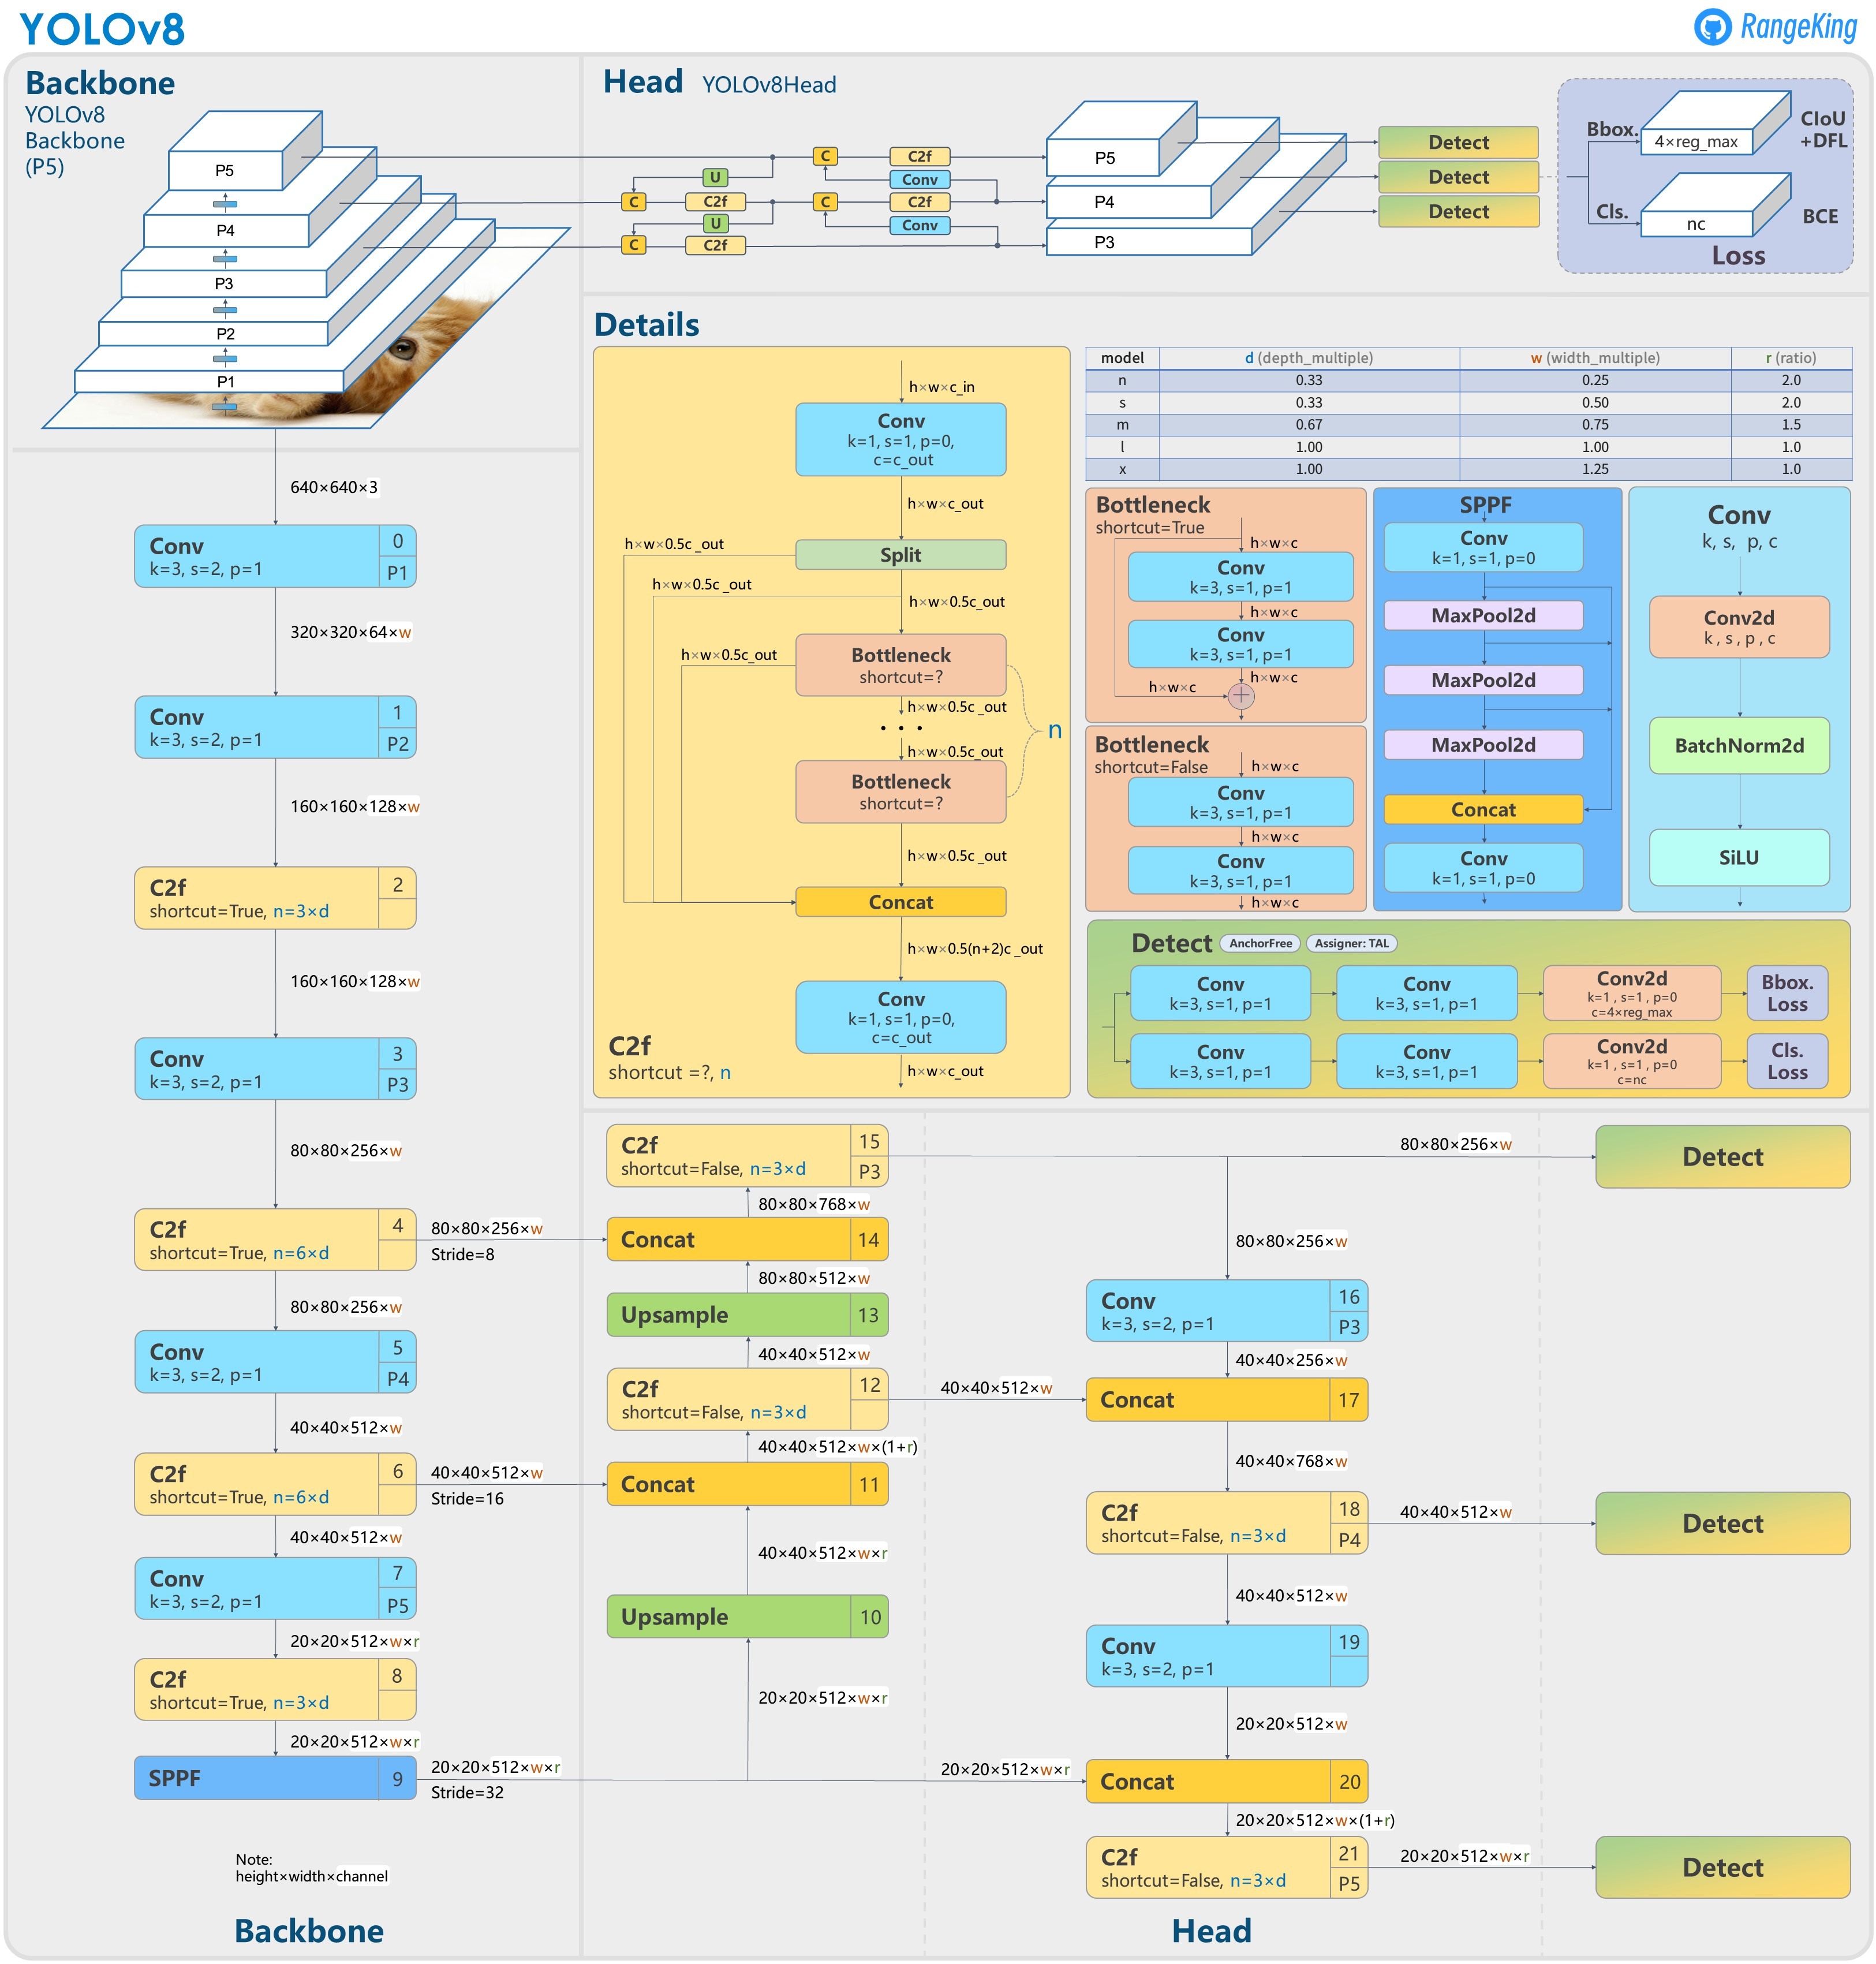
\includegraphics[width=\textwidth]{yolov8_architecture.jpg}
    \caption{Schema dell'architettura di YOLOv8}
    \label{fig:2}
\end{figure}

Il modello YOLOv8 incorpora anche una \textit{Neck} e una \textit{Head} ottimizzati per massimizzare la capacità di rilevamento attraverso una migliore aggregazione delle caratteristiche e una maggiore flessibilità nelle predizioni finali. L'uso di meccanismi come le \textit{Depthwise Separable Convolutions} contribuisce a ridurre il numero di operazioni computazionali, mantenendo un'elevata capacità espressiva del modello.

\subsection*{Dimensioni delle architetture usate}

Nell'ambito del progetto, si è scelto di utilizzare le varianti \textbf{small}, \textbf{medium} e \textbf{nano} di YOLOv8 per il task di object detection, in quanto queste architetture offrono un buon compromesso tra capacità computazionale e performance, risultando particolarmente adatte per l'esecuzione su hardware con risorse limitate quali quelle a noi disponibili.

\subsection*{Vantaggi di YOLOv8 per il Riconoscimento dei Rifiuti Plastici}

La scelta di YOLOv8 per il riconoscimento dei rifiuti plastici nei fiumi è giustificata da diversi fattori:

\begin{itemize}
    \item \textbf{Rilevamento in Tempo Reale}: YOLOv8 è noto per la sua capacità di eseguire object detection in tempo reale, il che è cruciale per applicazioni di monitoraggio continuo nei fiumi. La possibilità di rilevare e classificare i rifiuti plastici in tempo reale consente interventi immediati, riducendo il rischio che i rifiuti possano propagarsi ulteriormente.
    
    \item \textbf{Efficienza Computazionale}: Le versioni di YOLO sono ottimizzate per girare su hardware con risorse limitate, come droni o sistemi embedded. Questo le rende particolarmente adatte per applicazioni sul campo, dove la potenza di calcolo potrebbe essere un vincolo.
    
    \item \textbf{Accuratezza Elevata}: Nonostante la sua velocità, YOLOv8 mantiene un'accuratezza competitiva grazie all'uso di tecniche avanzate come l'addestramento con \textit{label smoothing} e l'adozione di una griglia più fine per la previsione delle bounding box. Questo è essenziale per distinguere efficacemente i rifiuti plastici da altri detriti naturali presenti nei fiumi, come è possibile vedere in un esempio alla figura \ref*{fig:3}.
\end{itemize}

\begin{figure}[h!]
    \centering
    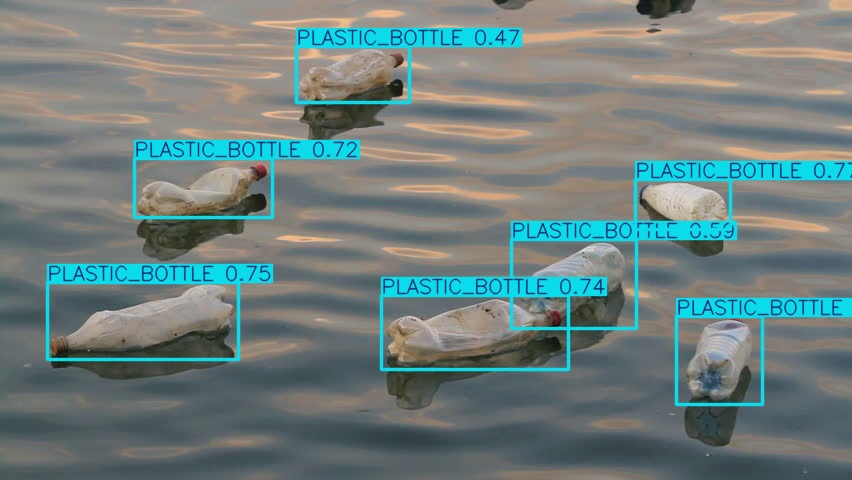
\includegraphics[width=\textwidth]{res_1203_1.jpg} 
    \caption{Esempio di output di YOLOv8 per il rilevamento di rifiuti plastici nei fiumi.}
    \label{fig:3}
\end{figure}


\section{Metriche per valutazione performance}

Nell'ambito del riconoscimento automatico dei rifiuti plastici nei fiumi utilizzando la rete convoluzionale YOLO (You Only Look Once), l'accurata valutazione delle performance del modello è cruciale. Il contesto operativo, caratterizzato da variabilità ambientali e la presenza di oggetti confondenti, rende fondamentale l'impiego di metriche di valutazione che forniscano una visione completa dell'efficacia del modello. In questa sezione, discuteremo in dettaglio le metriche principali utilizzate per valutare il modello, giustificando la loro rilevanza rispetto all'obiettivo specifico di riconoscimento dei rifiuti plastici.

\subsection*{Precision}

La \textit{Precision} è una metrica fondamentale nel contesto del riconoscimento dei rifiuti plastici. Questa misura indica la percentuale di rifiuti classificati correttamente tra tutti quelli identificati come rifiuti dal modello. In altre parole, la precision ci dice quanto possiamo fidarci delle predizioni positive effettuate da YOLO. La formula per calcolarla è la seguente:
\begin{equation}
\text{Precision} = \frac{TP}{TP + FP}
\end{equation}
dove:
\begin{itemize}
    \item \textit{TP} (True Positive): il numero di rifiuti plastici correttamente rilevati dal modello;
    \item \textit{FP} (False Positive): il numero di oggetti non plastici erroneamente identificati come rifiuti plastici.
\end{itemize}

Nel contesto dei fiumi, dove possono essere presenti detriti naturali o altre forme di inquinamento, una precision elevata è essenziale per ridurre i falsi allarmi. Un'elevata precision significa che il modello è in grado di distinguere efficacemente i rifiuti plastici da altri oggetti, riducendo il rischio di identificare erroneamente materiali innocui come inquinanti, il che è cruciale per evitare sprechi di risorse in operazioni di pulizia.

\subsection*{Recall}

La \textit{Recall} misura la capacità del modello di identificare correttamente tutti i rifiuti plastici presenti. La recall è particolarmente importante in scenari dove la priorità è minimizzare il numero di rifiuti plastici non rilevati (falsi negativi), che possono avere un impatto ambientale significativo se lasciati nei corsi d'acqua. La formula per calcolare la recall è la seguente:
\begin{equation}
\text{Recall} = \frac{TP}{TP + FN}
\end{equation}

Nel contesto del riconoscimento dei rifiuti plastici, un alto valore di recall significa che il modello è efficace nel rilevare la maggior parte dei rifiuti, riducendo al minimo il rischio che rifiuti plastici possano sfuggire all'attenzione. Tuttavia, un aumento della recall potrebbe portare a una diminuzione della precision, poiché il modello potrebbe iniziare a classificare erroneamente più oggetti come plastica per evitare di perdere i rifiuti effettivi. Pertanto, è fondamentale trovare un equilibrio tra precision e recall.

\subsection*{F1-Score}

L'\textit{F1-Score} è la media armonica tra precision e recall, offrendo una misura bilanciata che tiene conto sia dei falsi positivi che dei falsi negativi. Questa metrica è particolarmente utile in scenari come il riconoscimento dei rifiuti plastici, dove il dataset può presentare classi sbilanciate e dove è importante non sovra-ottimizzare il modello per una sola metrica a scapito dell'altra. La formula per l'F1-Score è:
\begin{equation}
F1 = \frac{2 \cdot \text{Precision} \cdot \text{Recall}}{\text{Precision} + \text{Recall}}
\end{equation}

Nel contesto del riconoscimento dei rifiuti plastici, l'F1-Score è \textbf{particolarmente indicato}, poiché consente di valutare l'efficacia complessiva del modello, bilanciando l'accuratezza con la capacità di rilevamento. Un F1-Score elevato indica che il modello YOLO è in grado di mantenere un buon equilibrio tra identificare correttamente i rifiuti plastici e minimizzare gli errori.

\subsection*{mean Average Precision (mAP)}

Il \textit{mean Average Precision} (mAP) è una delle metriche più utilizzate e riconosciute nella valutazione delle performance di modelli di \textit{object detection}. Il mAP rappresenta la media delle \textit{Average Precision} (AP) calcolate su tutte le classi considerate nel modello. La \textit{Average Precision}, a sua volta, è l'area sotto la curva Precision-Recall per ciascuna classe. Il mAP è particolarmente rilevante per il nostro caso di studio, poiché:

\begin{itemize}
    \item Riflette le prestazioni complessive del modello su più classi di rifiuti plastici (se categorizzati in diverse tipologie);
    \item Tiene conto della capacità del modello di rilevare i rifiuti plastici in condizioni variabili, come differenti condizioni di illuminazione, presenza di acqua torbida, e variazioni nella forma e dimensione dei rifiuti;
    \item Considera le variazioni nella soglia di rilevamento del modello, fornendo un'indicazione della sua robustezza e capacità di generalizzazione.
\end{itemize}

Nel caso del riconoscimento dei rifiuti plastici, un mAP elevato indica che il modello è in grado di rilevare correttamente i rifiuti in diverse situazioni operative, mantenendo un buon equilibrio tra precisione e richiamo per ciascuna classe considerata. Questo è cruciale per garantire che il sistema di monitoraggio automatico sia affidabile in ambienti reali e possa contribuire efficacemente alla riduzione dell'inquinamento nei corsi d'acqua.

\section{Esperimenti effettuati}

In questa sezione vengono esposti i vari esperimenti di addestramento svolti con annessi 
risultati e considerazioni.

\subsection*{Modello 1: v8m12 e v8m12bis}

% Introduzione su strategia del training -> qual è l'obiettivo dell'esperimento?
I primi esperimenti sono serviti per raccogliere informazioni utili per avere un fase di 
addestramento che fosse il più efficacie possibile. Innanzitutto si è cercato di capire quanto
tempo avrebbe ogni iterazione, ogni epoca e in genere l'addestramento richiesto e capire 
in particolare quante risorse computazionali erano richieste e quante epoche consentire
al modello durante la fase di training.

Questi test, così come molti dei seguenti esperimenti, sono stati eseguiti su un notebook
jupiter eseguito su server colab, sfruttando l'accelerazione GPU, in genere una scheda T4, 
fornita giornalmente per un massimo di 3 ore da parte di Google.

% Dettagli configurazione, tipologia modello e iperparametri

Una delle prime prove svolte riguarda due esecuzioni di training denominate durante il lavoro
\verb+v8m12+ e \verb+v8m12bis+. La prima è stata un'esecuzione di sole 30 epoche per vedere quanto 
velocemente le funzioni di loss scendessero di valore e stimare quante epoche concedere successivamente.
Il modello utilizzato è quello medio preaddestrato con il dataset COCO, come disponibile dalla libreria 
di ultralytics (YOLOv8m.pt).
La seconda esecuzione ha visto sempre un numero di epoche pari a 30 ma utilizzando come modello di
partenza il miglior modello dell'addestramento precedente in quanto dai risultati come è possibile vedere 
nella figura \ref{fig:v1-1} c'era ancora margine di miglioramento.

\begin{figure}[h]
    \centering
    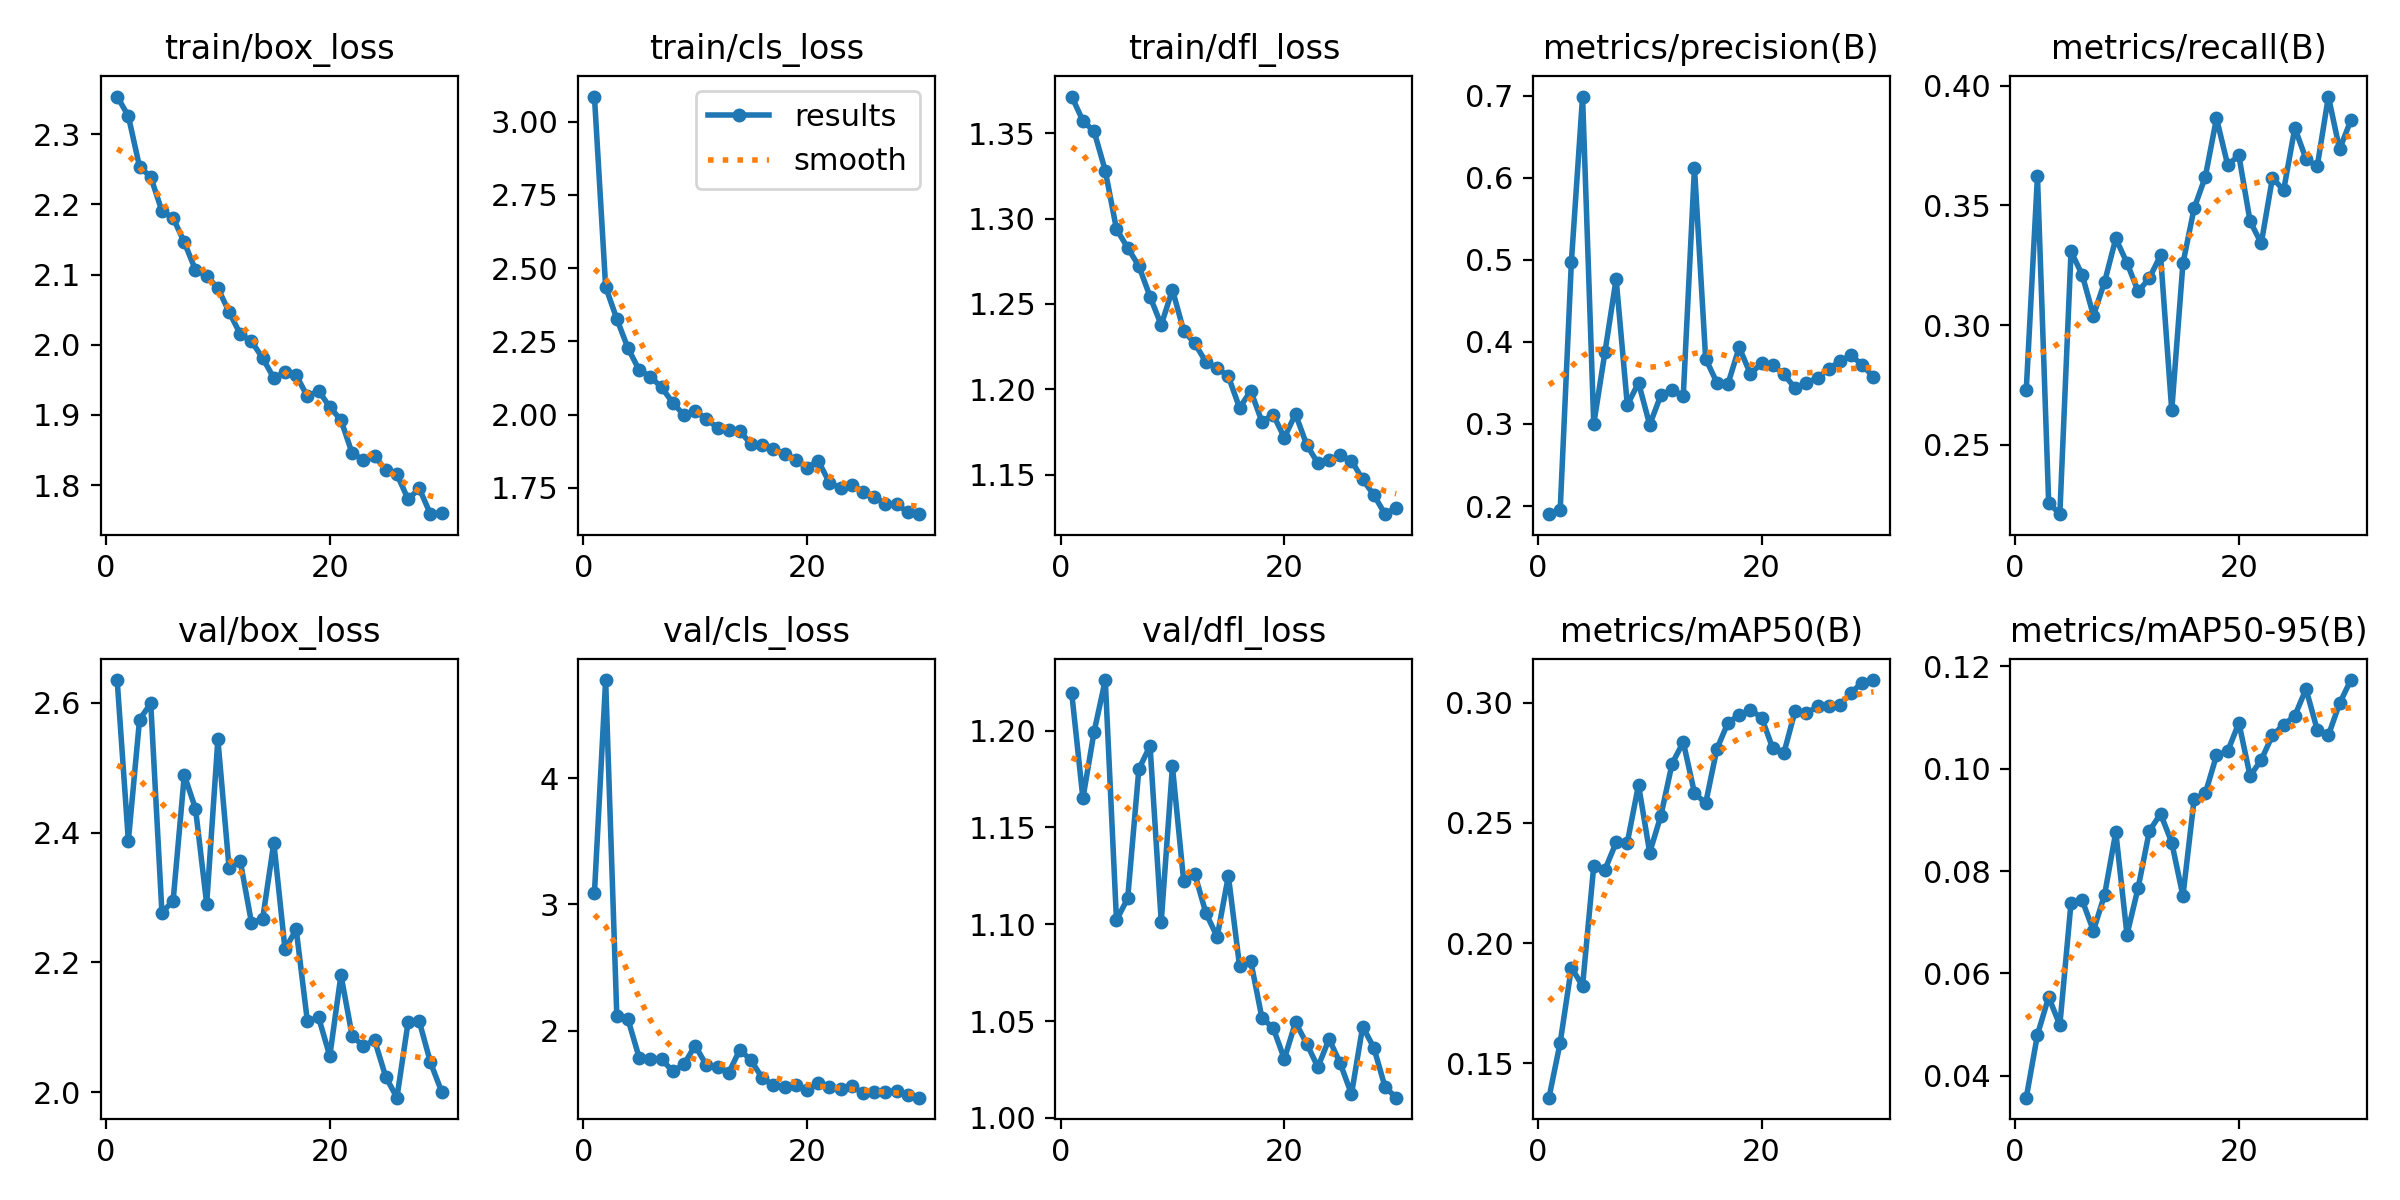
\includegraphics[width=0.8\textwidth]{v_1/results.png}
    \caption{Andamento funzioni di loss e metriche durante l'esecuzione di \texttt{v8m12}}
    \label{fig:v1-1}
    \end{figure}

Molti degli iperparametri, se non tutti, sono stati tenuti quelli di default della libreria di ultralytics.
L'unico iperparametro impostato per curiosità è \verb|freeze|: in breve abbiamo tenuto 7 layer del modello 
di YOLO congelati in modo da ridurre il tempo necessario per l'addestramento. Per la bontà dell'esperimento
si è dimostrato di poca utilità e gli addestramenti successivi tale iperparametro è stato ignorato, 
ovvero la modifica dei pesi avveniva su tutto il modello.

% Risultati training
    % - andamento training
    % - grafici recall e precision e performance e F1
    % - matrici di confusione
    % - tabella performance test set

% Commento risultati

In ogni caso a prescindere dai risultati ottenuti, che per la natura dell'esperimento non sono
fondamentali, si è visto come il numero di epoche necessario per 
l'addestramento dovrebbe essere molto più alto per poter raggiungere quanto meno un'efficacia del modello
accettabile, così come è stato fatto poi per gli esperimenti successivi.
\subsection*{Modello 2 - small-1202 e small-1203}

% Introduzione su strategia del training -> qual è l'obiettivo dell'esperimento?
Avendo sperimentato con i vari modelli, abbiamo iniziato a effettuare alcuni addestramenti aumentando il
numero di epoche. Si è deciso quindi di procedere con il training su tutti i parametri della rete e non
congelare alcuni layer con l'opzione \verb|freeze| ma bilanciando l'operazione optando per la dimensione
del modello più piccola quale la versione small YOLOv8s. Il numero di epoche per esecuzione è stato impostato a 120 e per tale motivo i vari modelli sono stati
nominati come \verb|small-120x|. 

Il primo dei due modelli, \verb|small-1202|, ha visto una esecuzione 
comunque non ottimale visto che alcuni dei valori di loss rispetto alla validazione non sono stati 
salvati per alcuni problemi durante l'esecuzione su colab. Ciononostante si è visto, come in figura
\ref{fig:v2-1}, che i valori delle funzioni di loss continuavano a decrescere mentre le metriche
o rimanevano costanti, come precision e recall, o andavano a migliorare, come mAP50.

\begin{figure}[h]
    \centering
    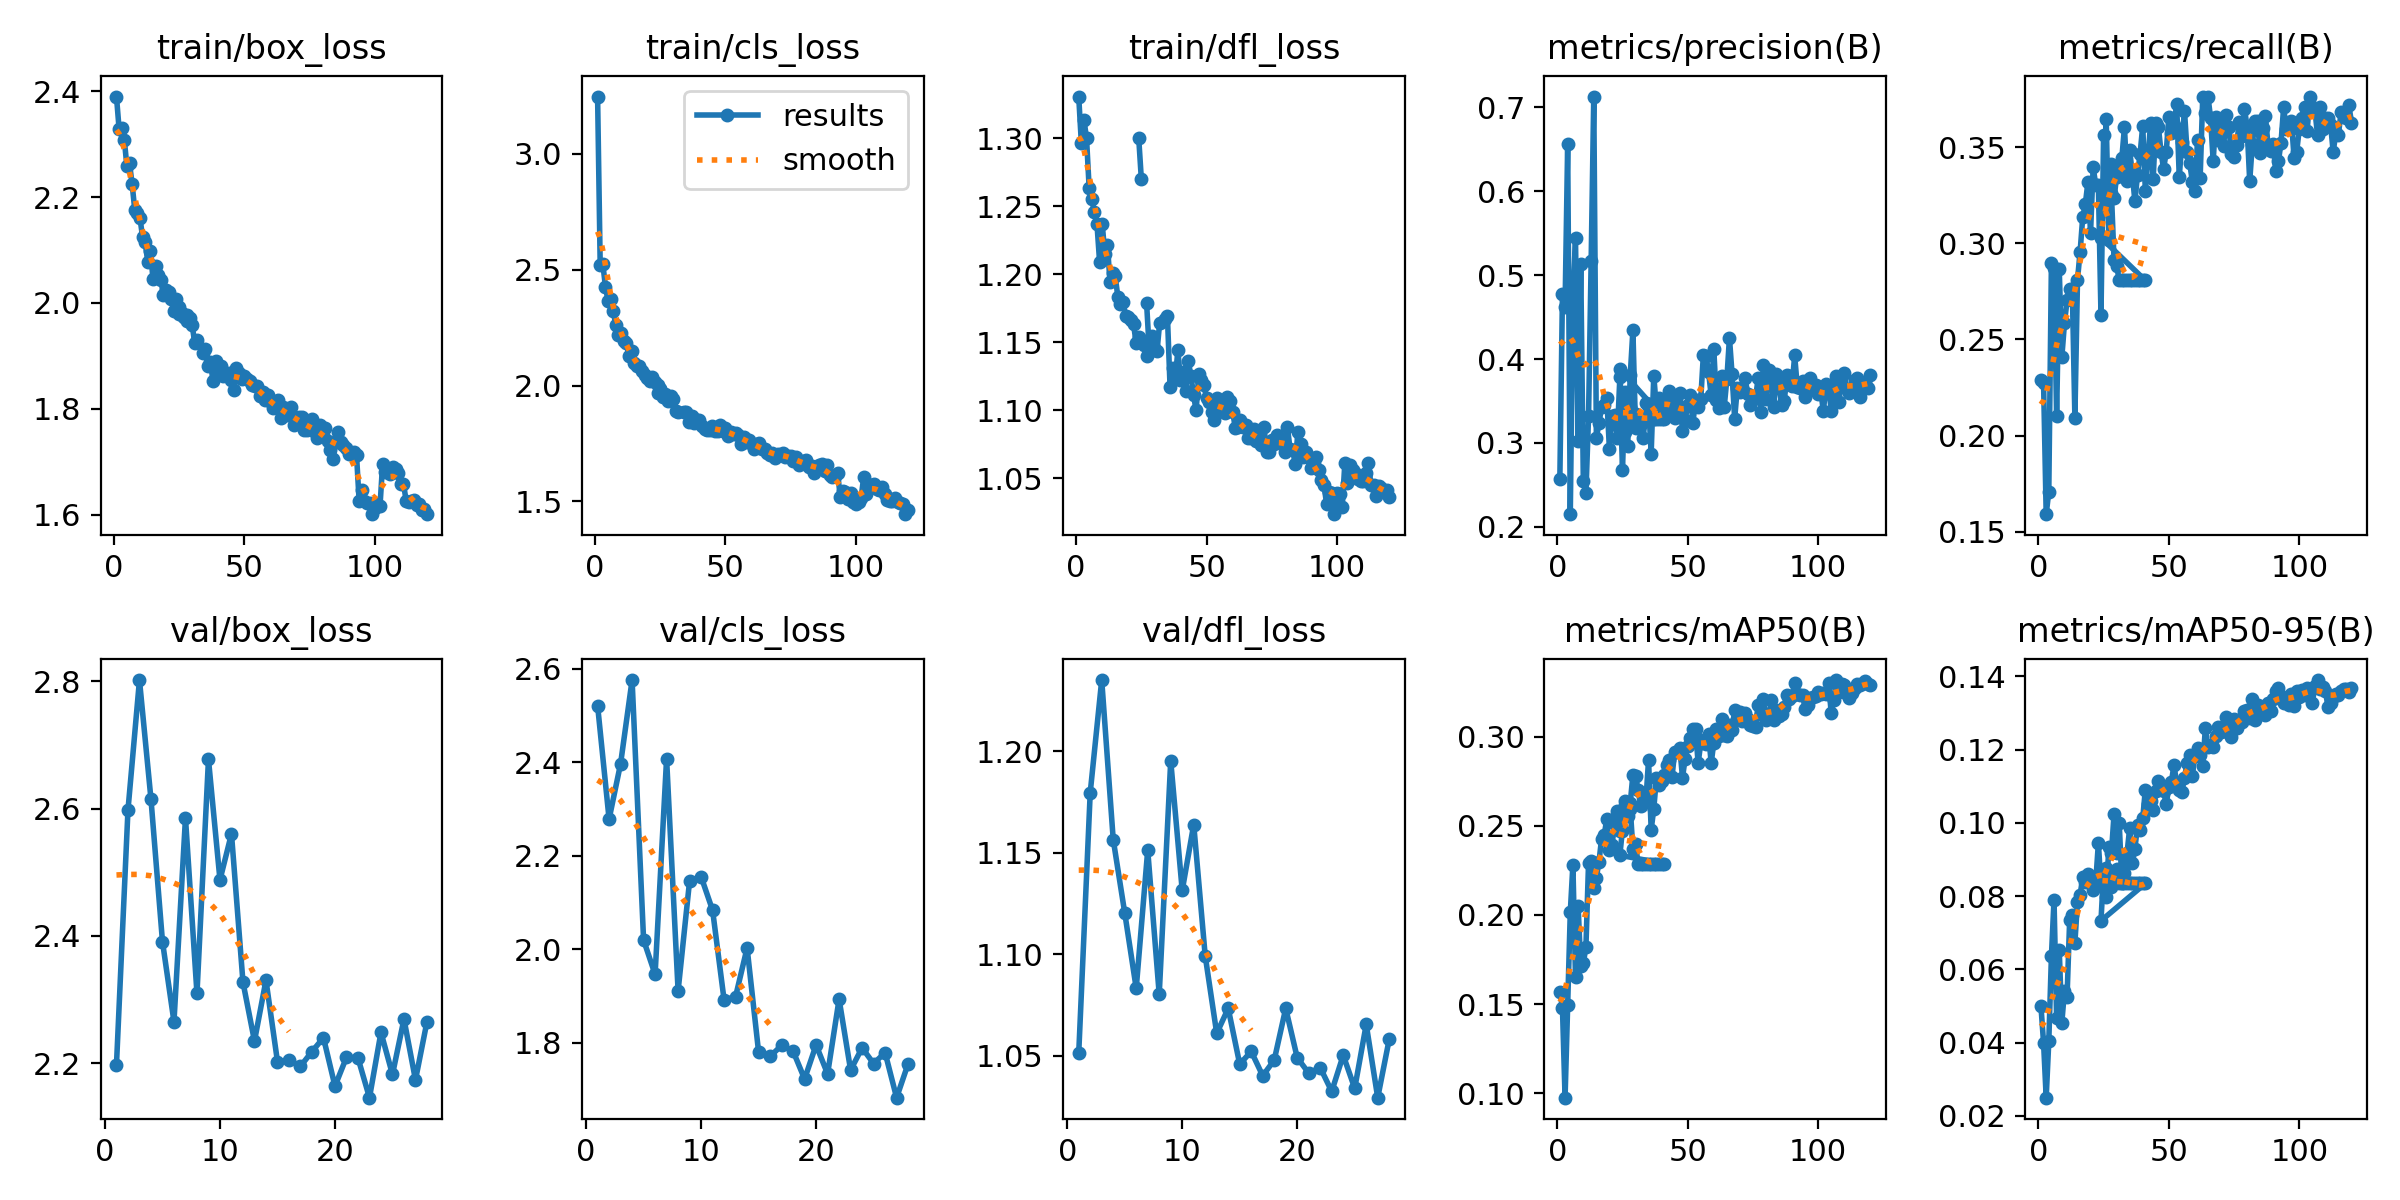
\includegraphics[width=0.8\textwidth]{v_2/small-1202/results.png}
    \caption{Andamento funzioni di loss e metriche durante l'esecuzione di \texttt{small-1202}}
    \label{fig:v2-1}
\end{figure}

La fase di training è stata pertanto ripetuta con l'esecuzione \verb|small-1203| che rispetto al nome assegnatogli
ha avuto 300 epoche a disposizione per l'addestramento mantenendo gli stessi iperparametri del tentativo precedente.

% Dettagli configurazione, tipologia modello e iperparametri, dove è stato eseguito il train
Di seguito sono riportati tutti gli iperparametri più importanti che caratterizzano questi addestramenti:

\begin{table}[h!]
    \centering
    \begin{tabular}{lc}
        \hline
        \textbf{Iperparametro} & \textbf{Valore} \\
        \hline
        epoche & 300  \\
        optimizer & auto (SGD) \\
        learning rate (lr0) & 0.01 \\
        learning rate (lrf) & 0.01 \\
        momentum & 0.937 \\
        weight\_decay & 0.0005 \\
        imgsz & 640 \\
        dropout & 0.15 \\
        patience & 100 \\
        \midrule
        hsv\_h & 0.7 \\
        degrees & 120 \\
        shear & 55 \\
        \hline
    \end{tabular}
    \caption{Configurazione iperparametri del modello \texttt{small-1203} per il training}
    \label{tab:v2-model-configs}
    \end{table}

In particolare da notare nella tabella \ref{tab:v2-model-configs} l'aggiunta dell'iperparametro \texttt{dropout} rispetto alla configurazione
del modello \texttt{small-1202} per poter introdurre una certa regolarizzazione all'interno della fase
di apprendimento. 
Abbiamo poi sfruttato il parametro \texttt{patience} che indica quante epoche aspettare
prima di effettuare early stopping nel caso in cui non ci fossero stati miglioramenti delle prestazioni.
% Risultati training
    % - andamento training

    \begin{figure}[!htb]
        \centering
        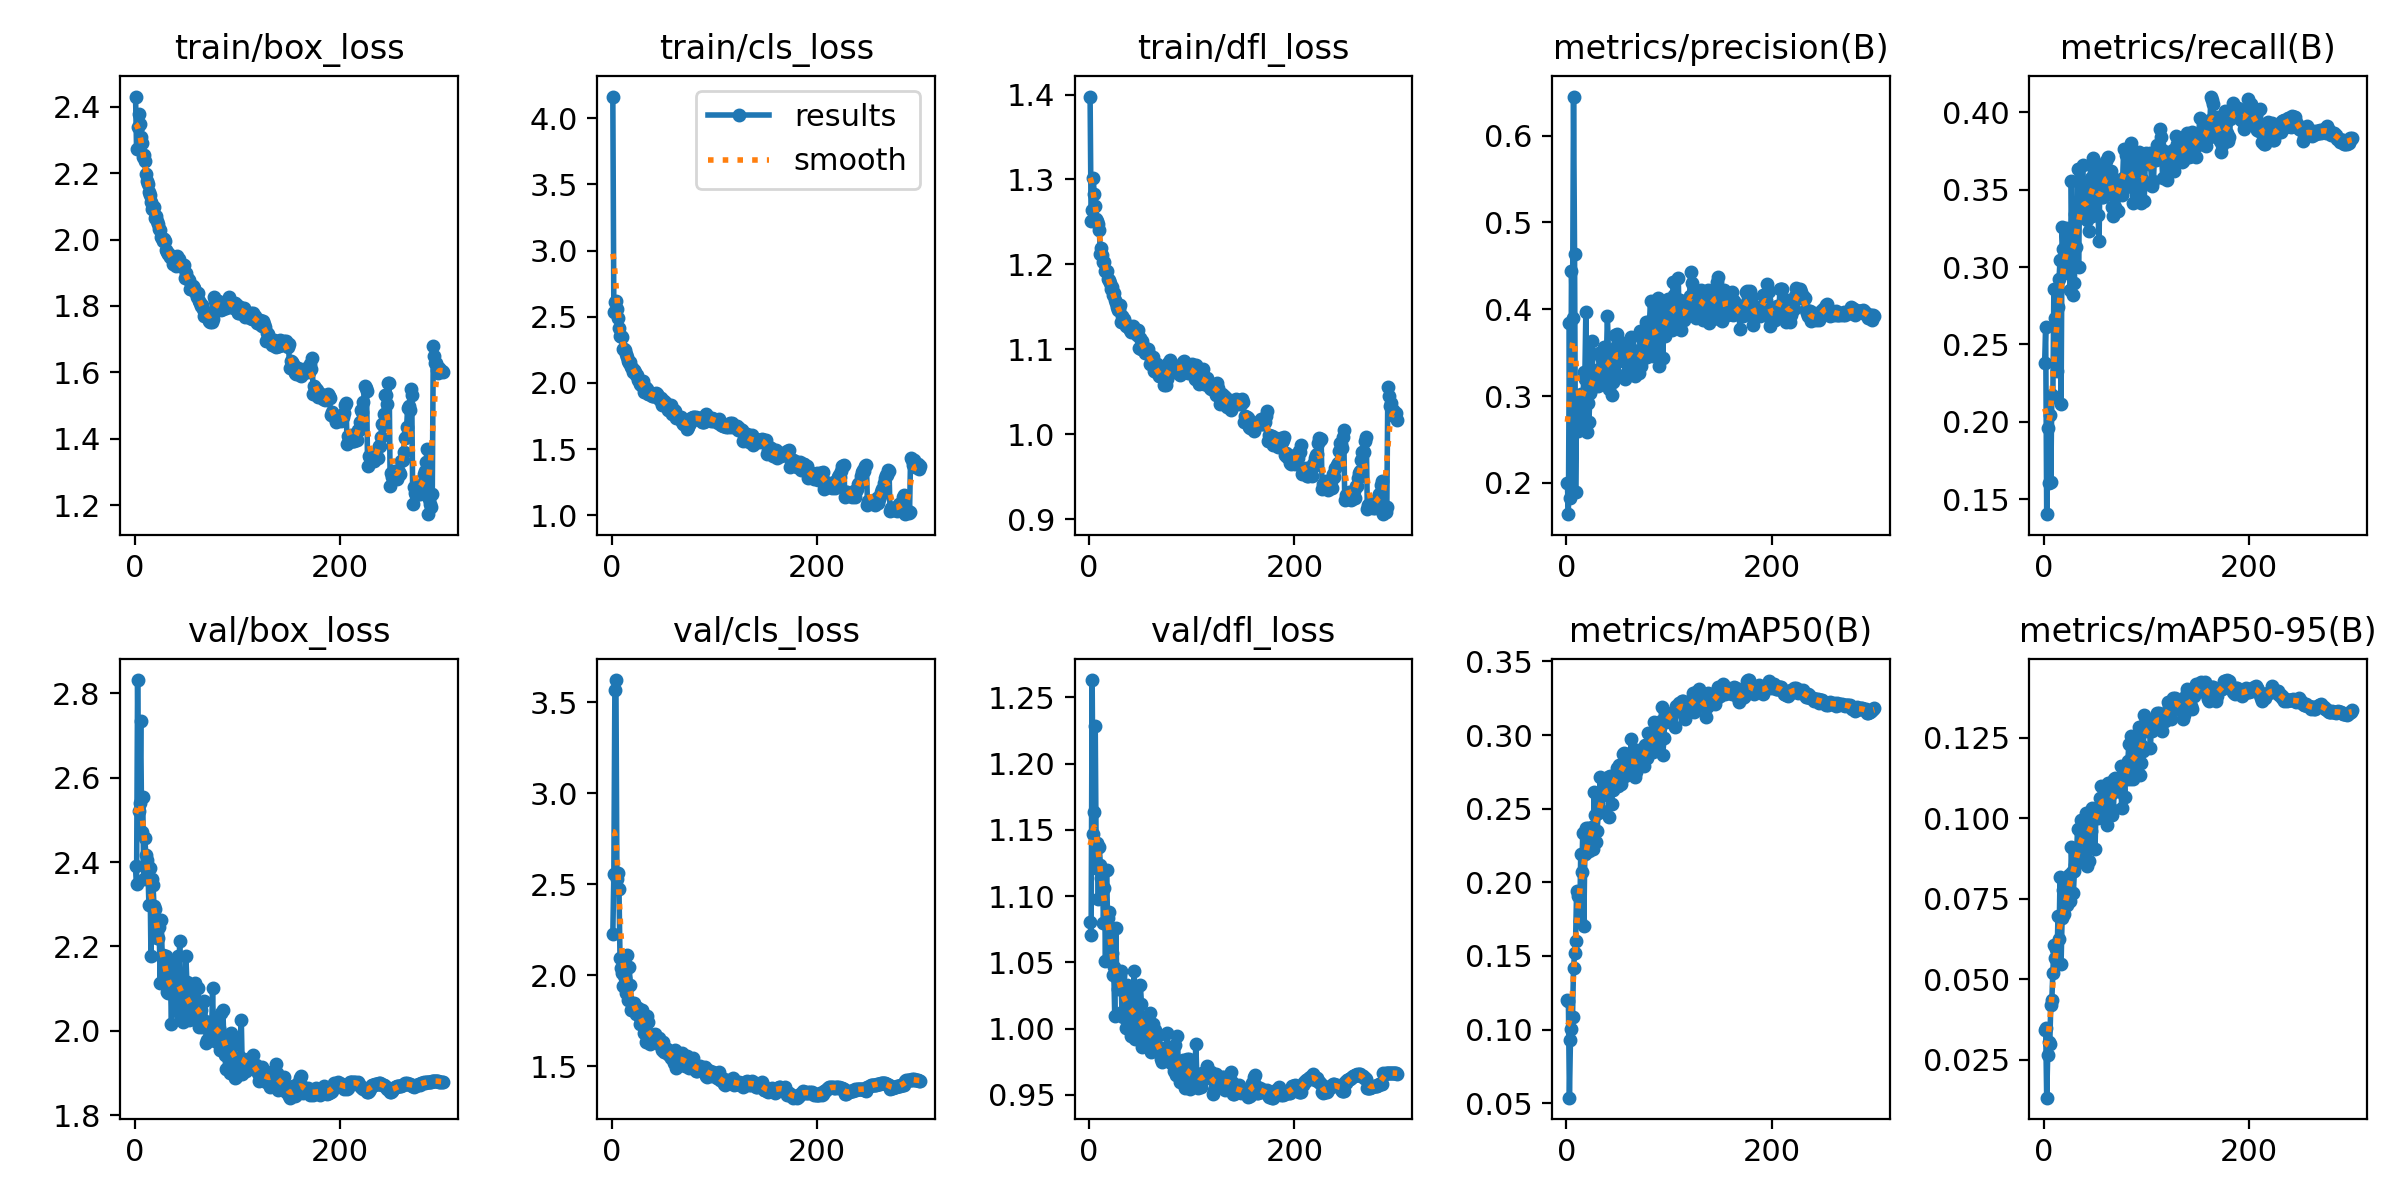
\includegraphics[width=0.8\textwidth]{v_2/small-1203/results.png}
        \caption{Andamento funzioni di loss e metriche durante l'esecuzione di \texttt{small-1203}}
        \label{fig:v2-2}
    \end{figure}
    % - grafici recall e precision e performance e F1
    \begin{figure}[!htb]
        \centering
        \begin{subfigure}{.5\textwidth}
            \centering
            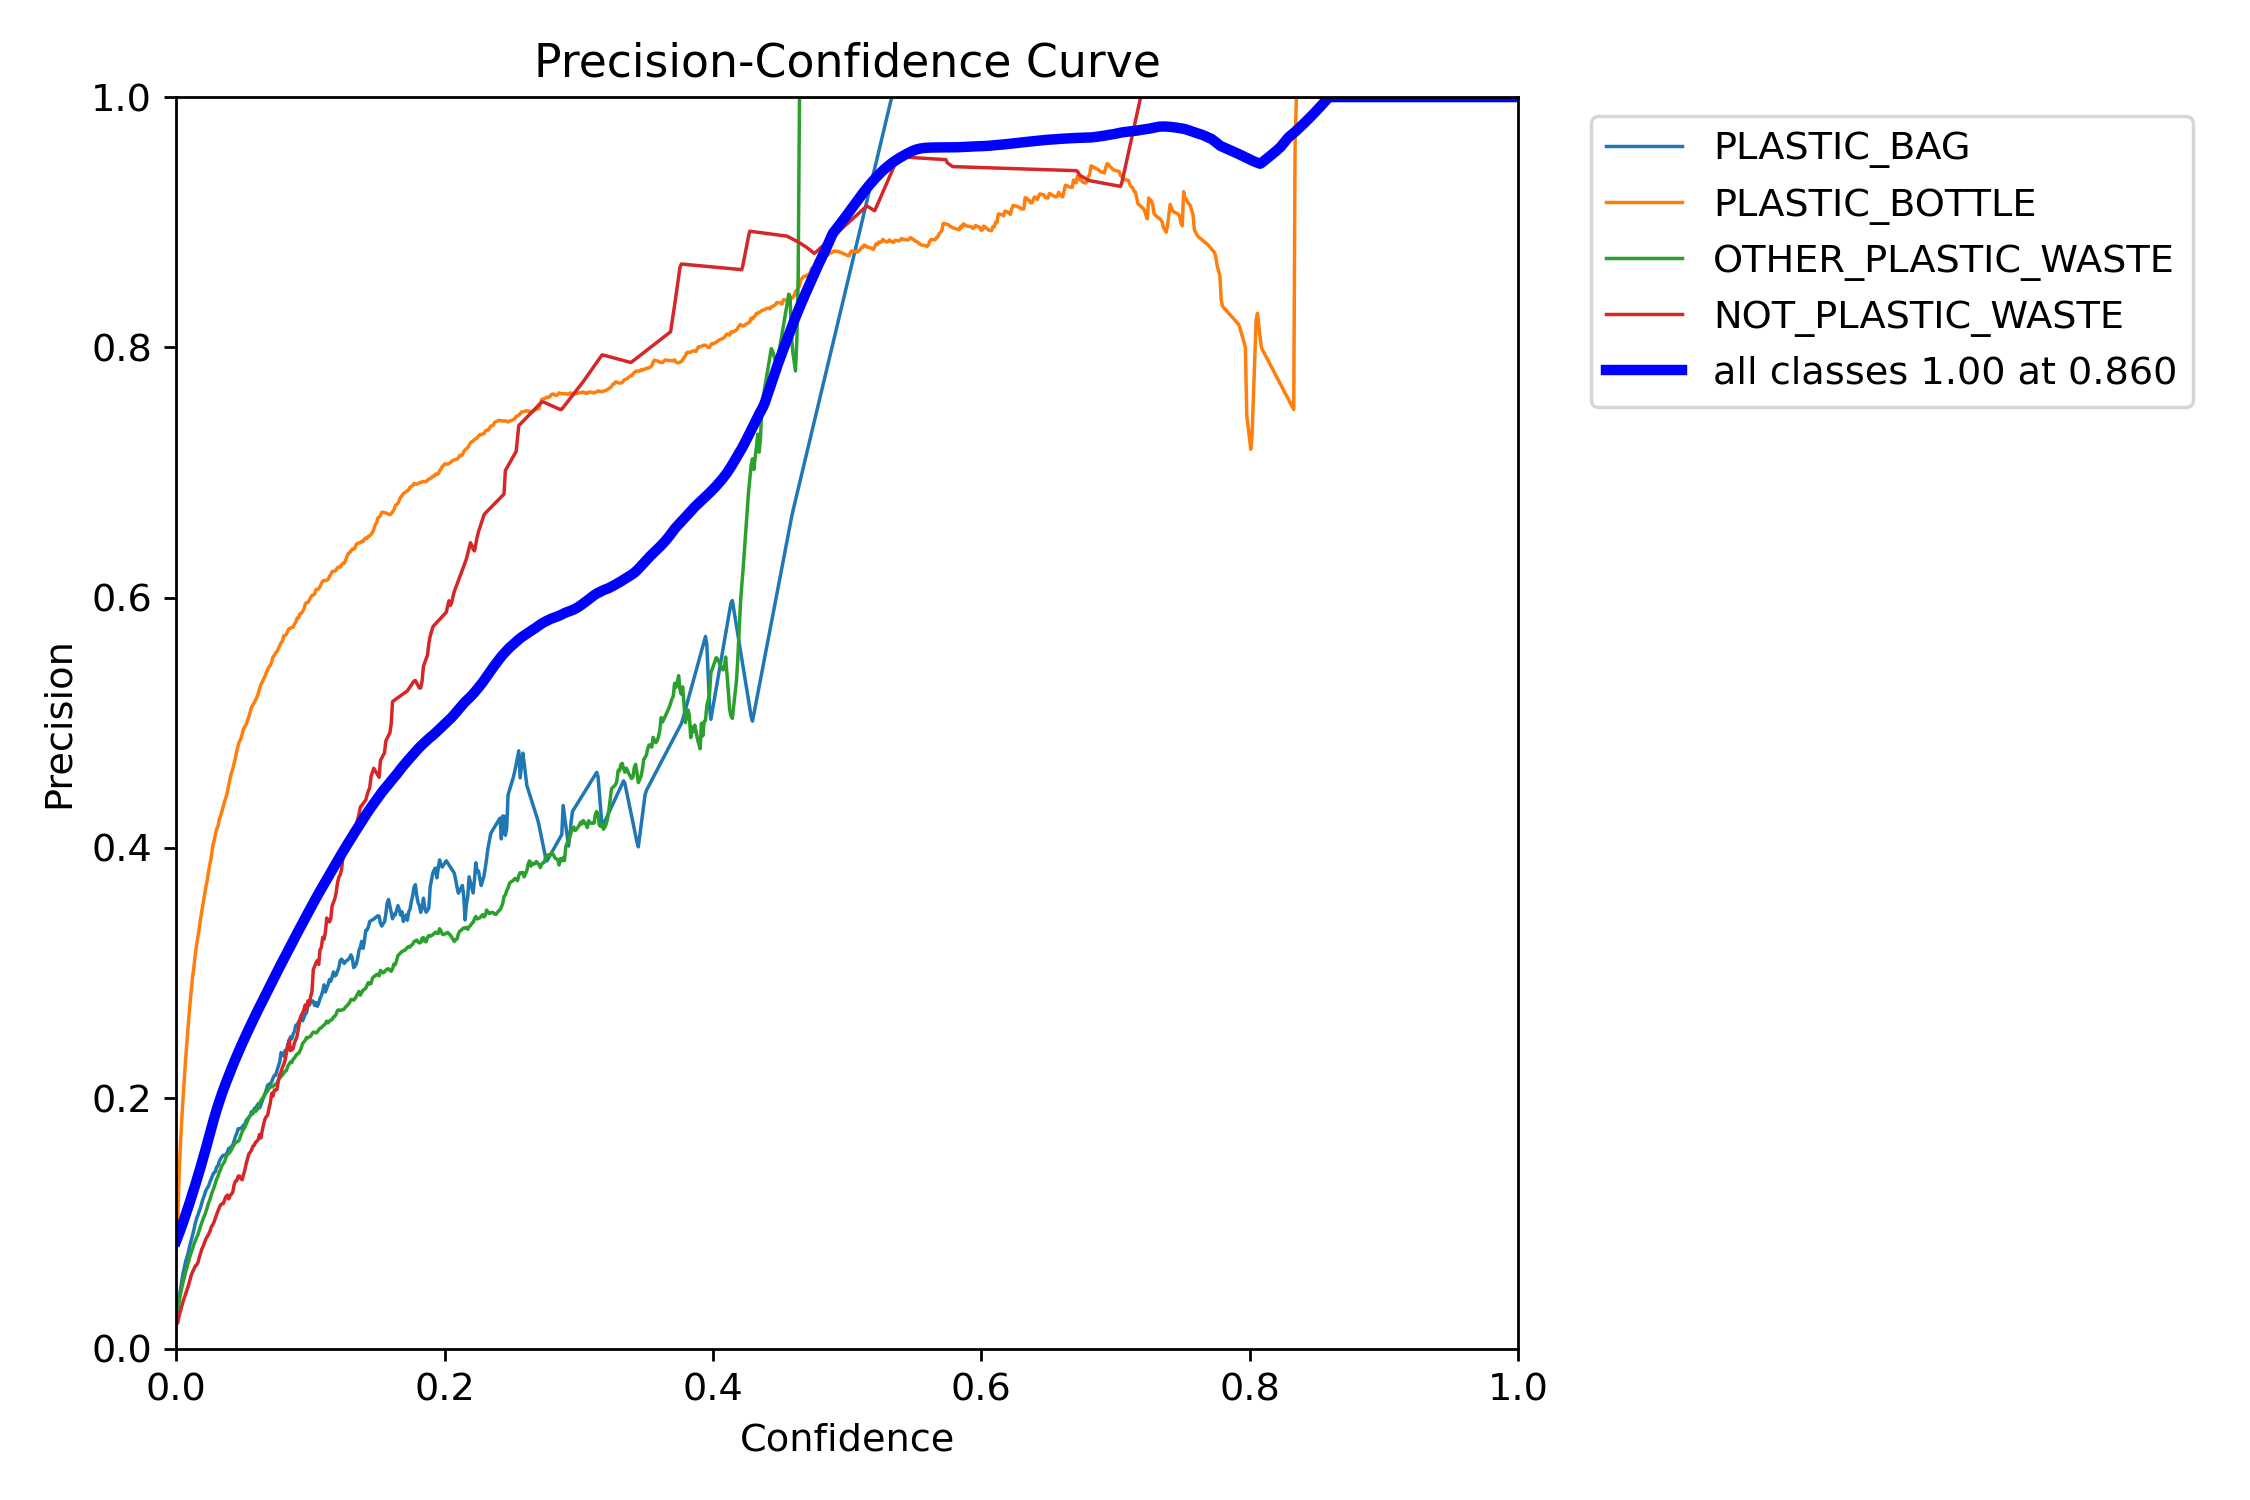
\includegraphics[width=.9\linewidth]{v_2/small-1203/P_curve.png}
            \subcaption{P-curve}
            \label{fig:v2-3.1}
          \end{subfigure}%
          \begin{subfigure}{.5\textwidth}
            \centering
            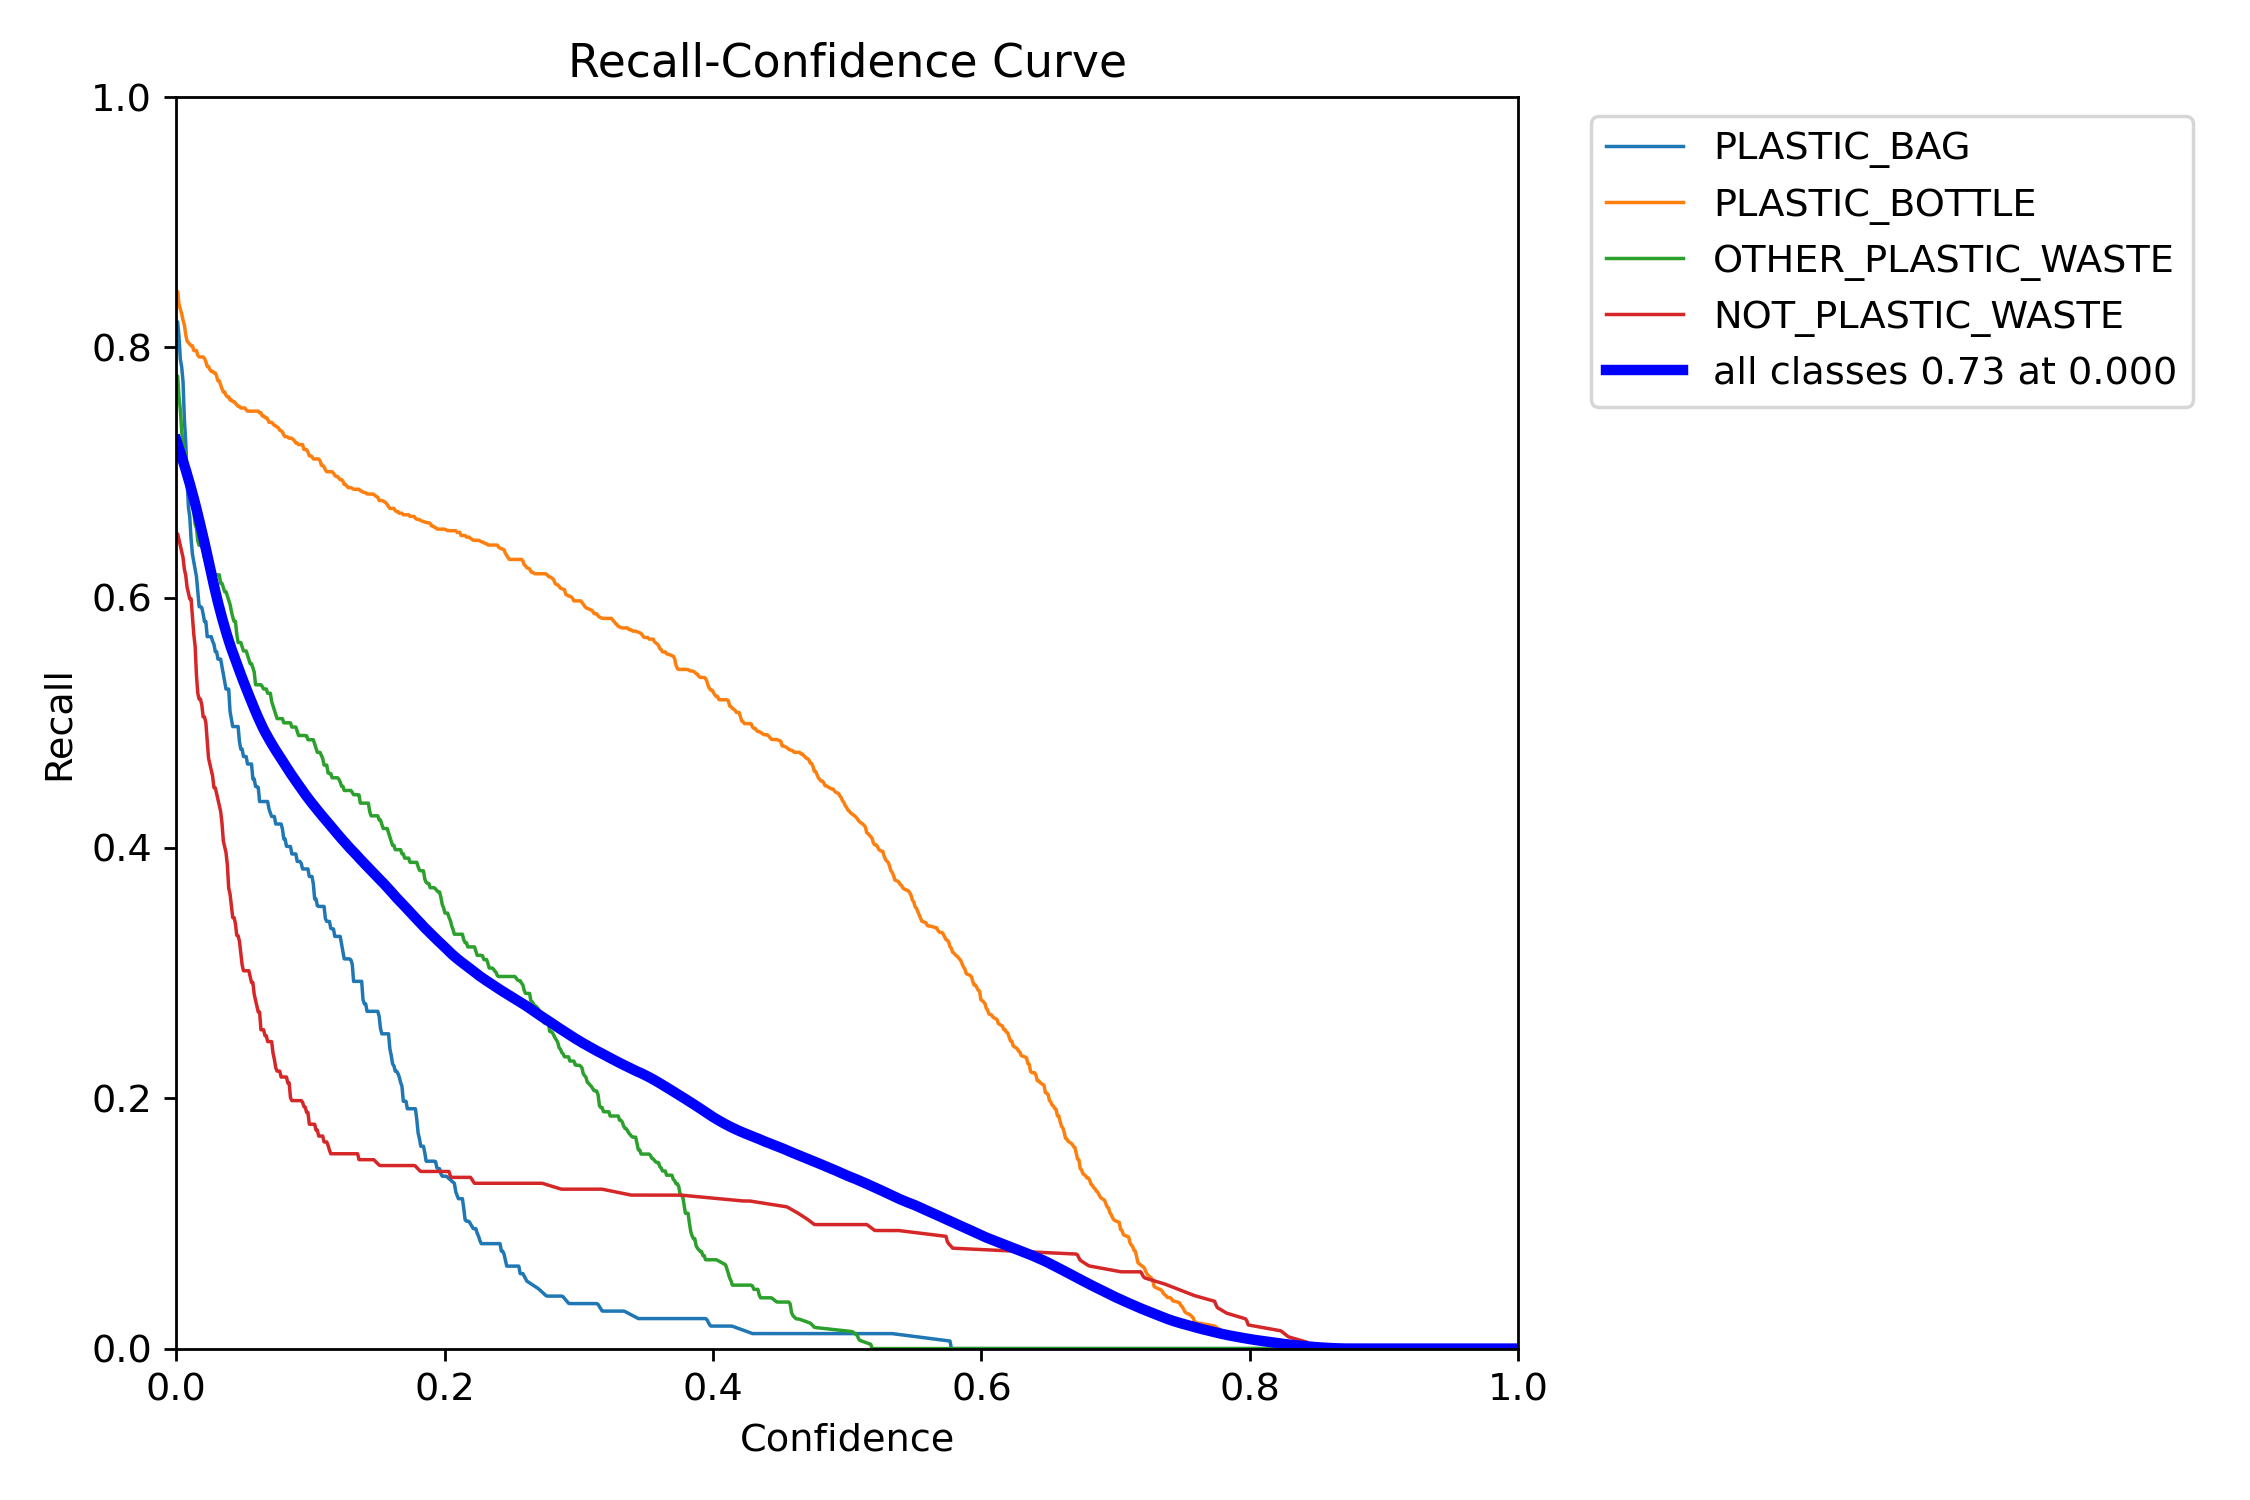
\includegraphics[width=.9\linewidth]{v_2/small-1203/R_curve.png}
            \subcaption{R-curve}
            \label{fig:v2-3.2}
          \end{subfigure}
          \vskip\baselineskip
        \begin{subfigure}{.5\textwidth}
          \centering
          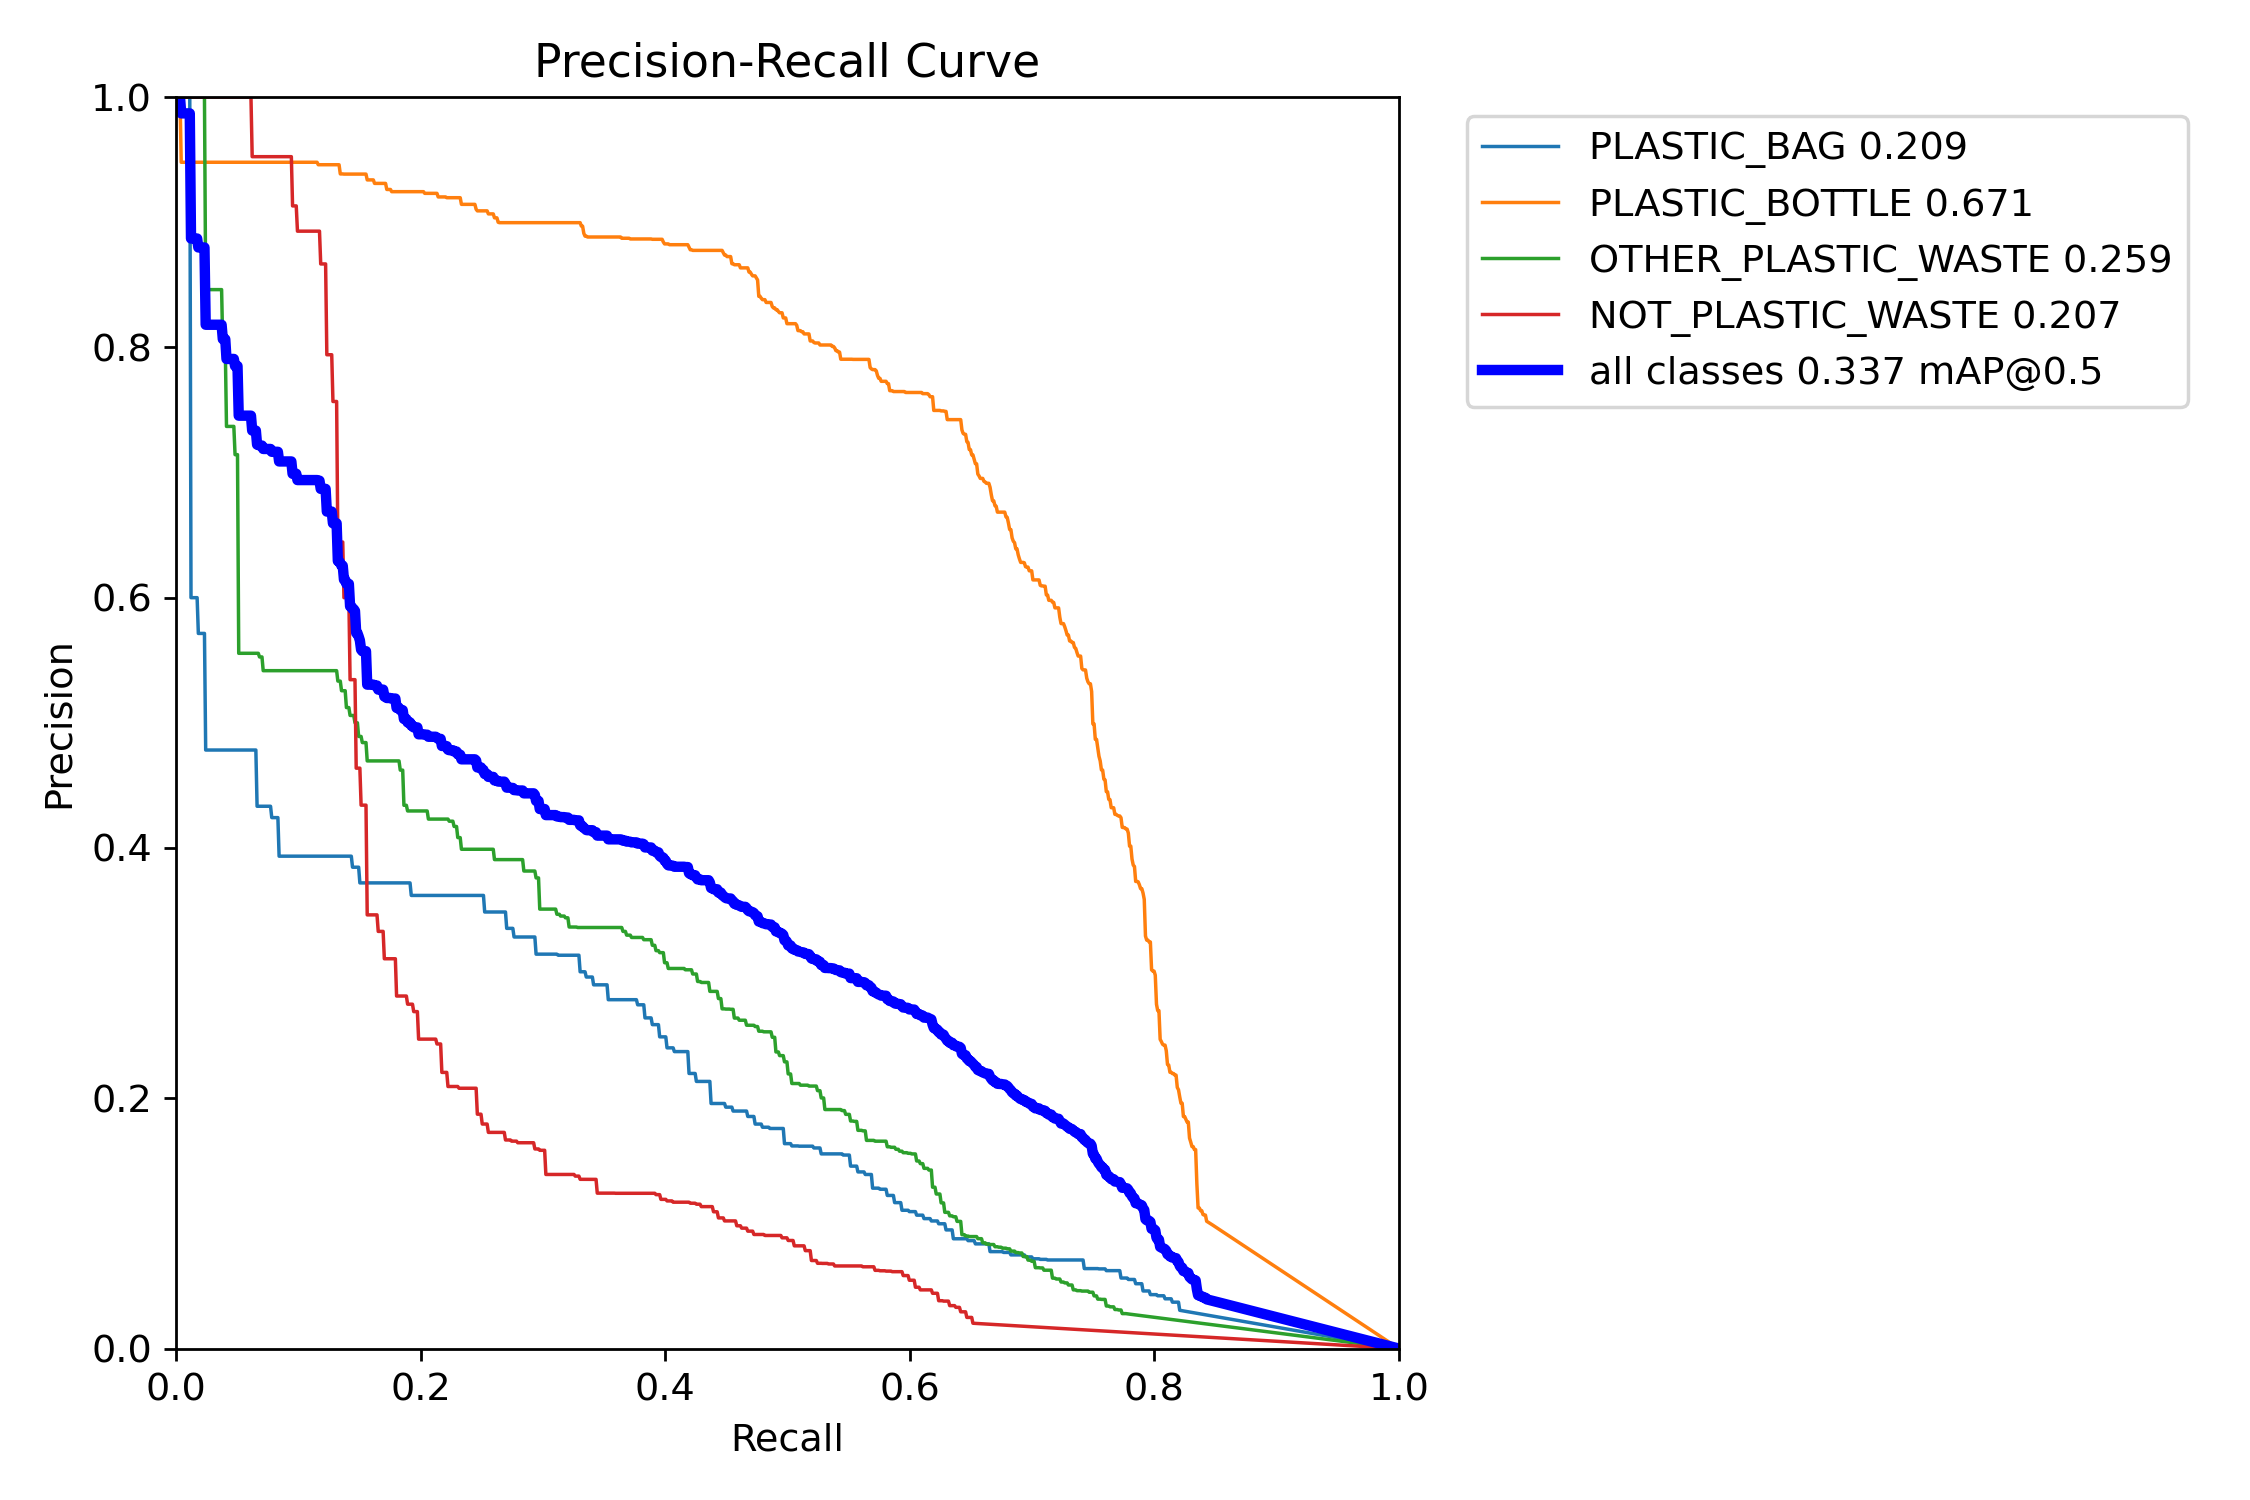
\includegraphics[width=.9\linewidth]{v_2/small-1203/PR_curve.png}
          \subcaption{PR-curve}
          \label{fig:v2-3.3}
        \end{subfigure}
        \begin{subfigure}{.49\textwidth}
            \centering
            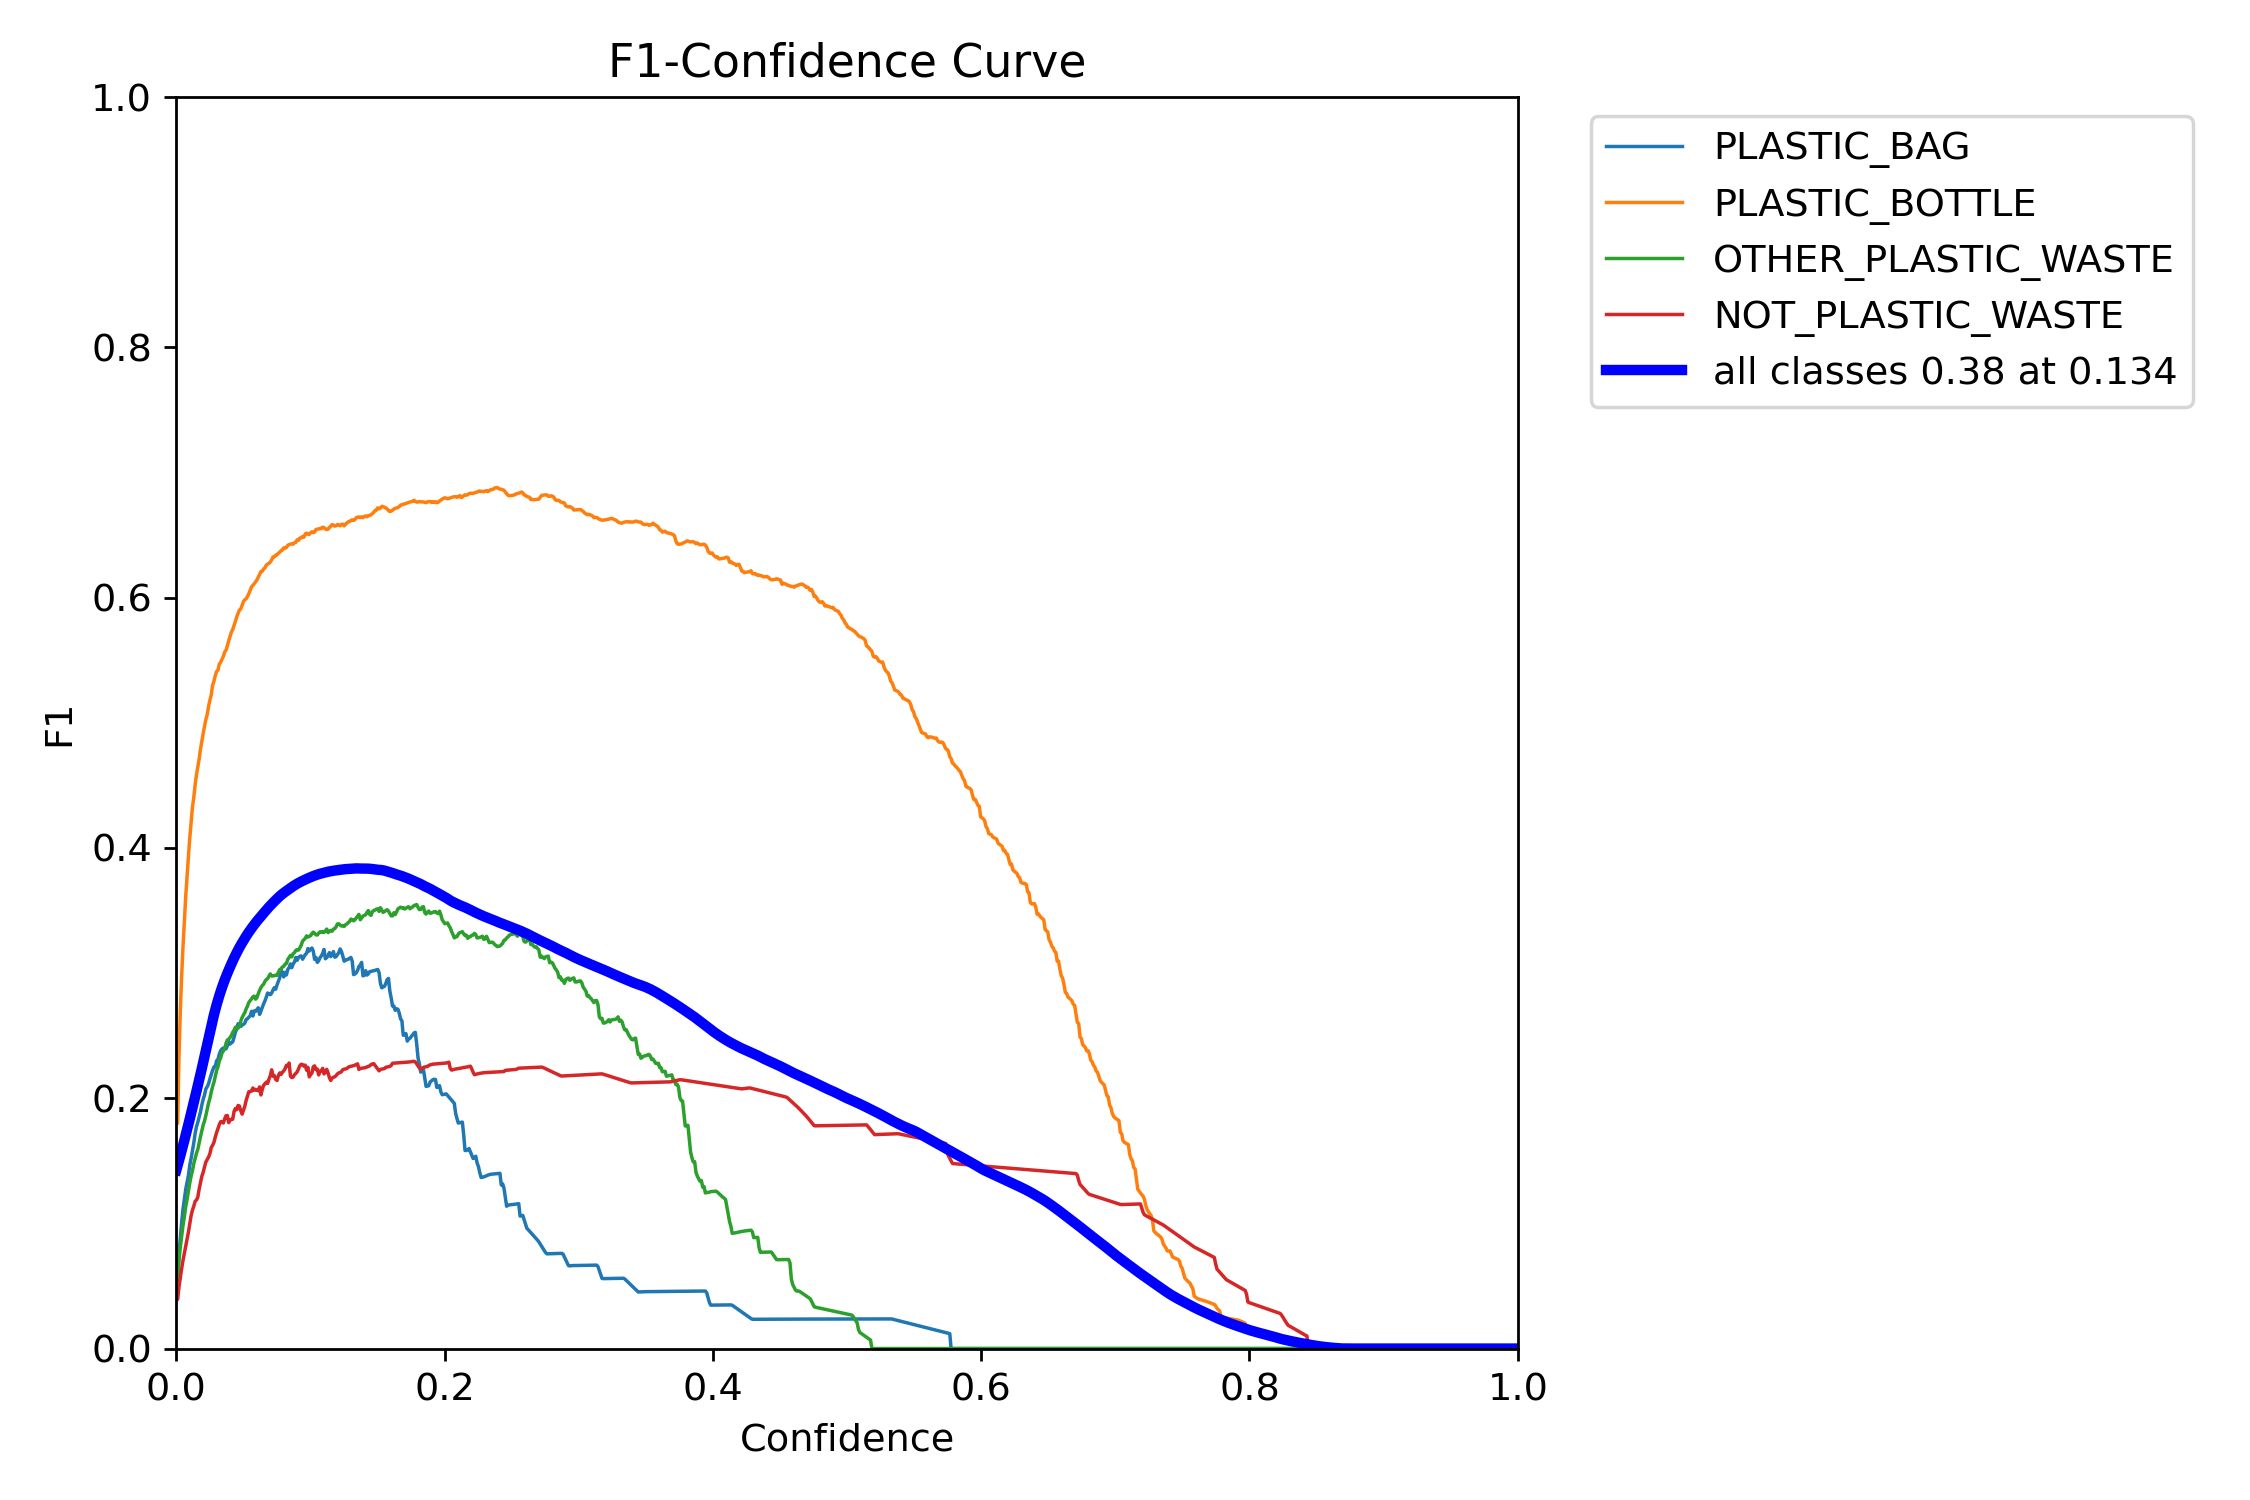
\includegraphics[width=.9\linewidth]{v_2/small-1203/F1_curve.png}
            \subcaption{F1-curve}
            \label{fig:v2-3.4}
          \end{subfigure}

        \caption{Da in alto a sinistra in poi, curva di confidenza della precisione, 
        curva di confidenza del richiamo, curva precisione-richiamo e
        curva di confidenza F1 per il modello \texttt{small-1203}}
        \label{fig:v2-3}
    \end{figure}


    % - matrici di confusione
    
    % - tabella performance test set

% Commento risultati
Quello che si è potuto vedere dai risultati e dalle performance di questi modelli, come è possibile
consultare dai grafici in figura \ref{fig:v2-2} e in tabella \ref{table:v2-1}, è che la rete
tende ad avere discreti precisione e richiamo ma non troppo soddisfacenti. 
In particolare se si considera una delle metriche più significative quali mAP50 vediamo che si 
raggiunge il valore nel caso migliore del 37.4\% che potrebbe essere sì considerato un risultato
accettabile ma che presenta alcuni dubbi sull'efficacia del modello. 

Considerando anche gli andamenti delle funzioni di errore durante l'addestramento (figura \ref{fig:v2-2}) si può notare
come i valori di loss con il set di validazione vengono plafonati mentre  quelli inerenti al 
training set in genere si riducono ma avendo un comportamento oscillante. Questo può indicare
un momento di stallo che può portare a un indesiderato overfitting della rete.

È anche possibile vedere dalla tabella \ref{table:v2-1} e dalla matrice di confusione normalizzata
in figura \ref{fig:v2-4} come la distribuzione sbilanciata delle classi comporta sì ottimi risultati
per la classe \texttt{PLASTIC\_BOTTLE} ma risultati discreti nelle altre se non addirittura pessime
considerando la classe \texttt{OTHER\_PLASTIC\_WASTE}. Questo fenomeno si è visto in tutti gli esperimenti
e non è stato possibile rimuoverlo ma solo arginarlo in parte.

Anche per quanto riguarda l'analisi delle curve di confidenza delle varie metriche, figura \ref{fig:v2-3},
si può notare come la classe \texttt{PLASTIC\_BOTTLE}, rappresentata dalle curve arancioni,
abbia performance nettamente migliori rispetto alla media.

Se il modello fosse pensato per il solo riconoscimento delle bottiglie di plastica probabilmente
si potevano raggiungere ottimi risultati ma di contro sarebbero stati poco utili poi all'atto 
pratico. 

\begin{table}[!htb]
    \centering
    \begin{tabularx}{\textwidth}{lYYYc}
        \toprule
        Class &  P & R & mAP50 & mAP50-95 \\
        \midrule
        ALL &  0.452 & 0.450 & 0.374 & 0.172 \\
        PLASTIC\_BAG &  0.402 & 0.388 & 0.344 & 0.120 \\
        PLASTIC\_BOTTLE & 0.684 & 0.727 & 0.724 & 0.344 \\
        OTHER\_PLASTIC\_WASTE & 0.140 & 0.377 & 0.106 & 0.0367 \\
        NOT\_PLASTIC\_WASTE & 0.582 & 0.306 & 0.320 & 0.187 \\
        \bottomrule
    \end{tabularx}
    \caption{Risultati delle metriche sul test set per \texttt{small-1203}}
    \label{table:v2-1}
\end{table}

\begin{figure}[htb!]
    \centering
    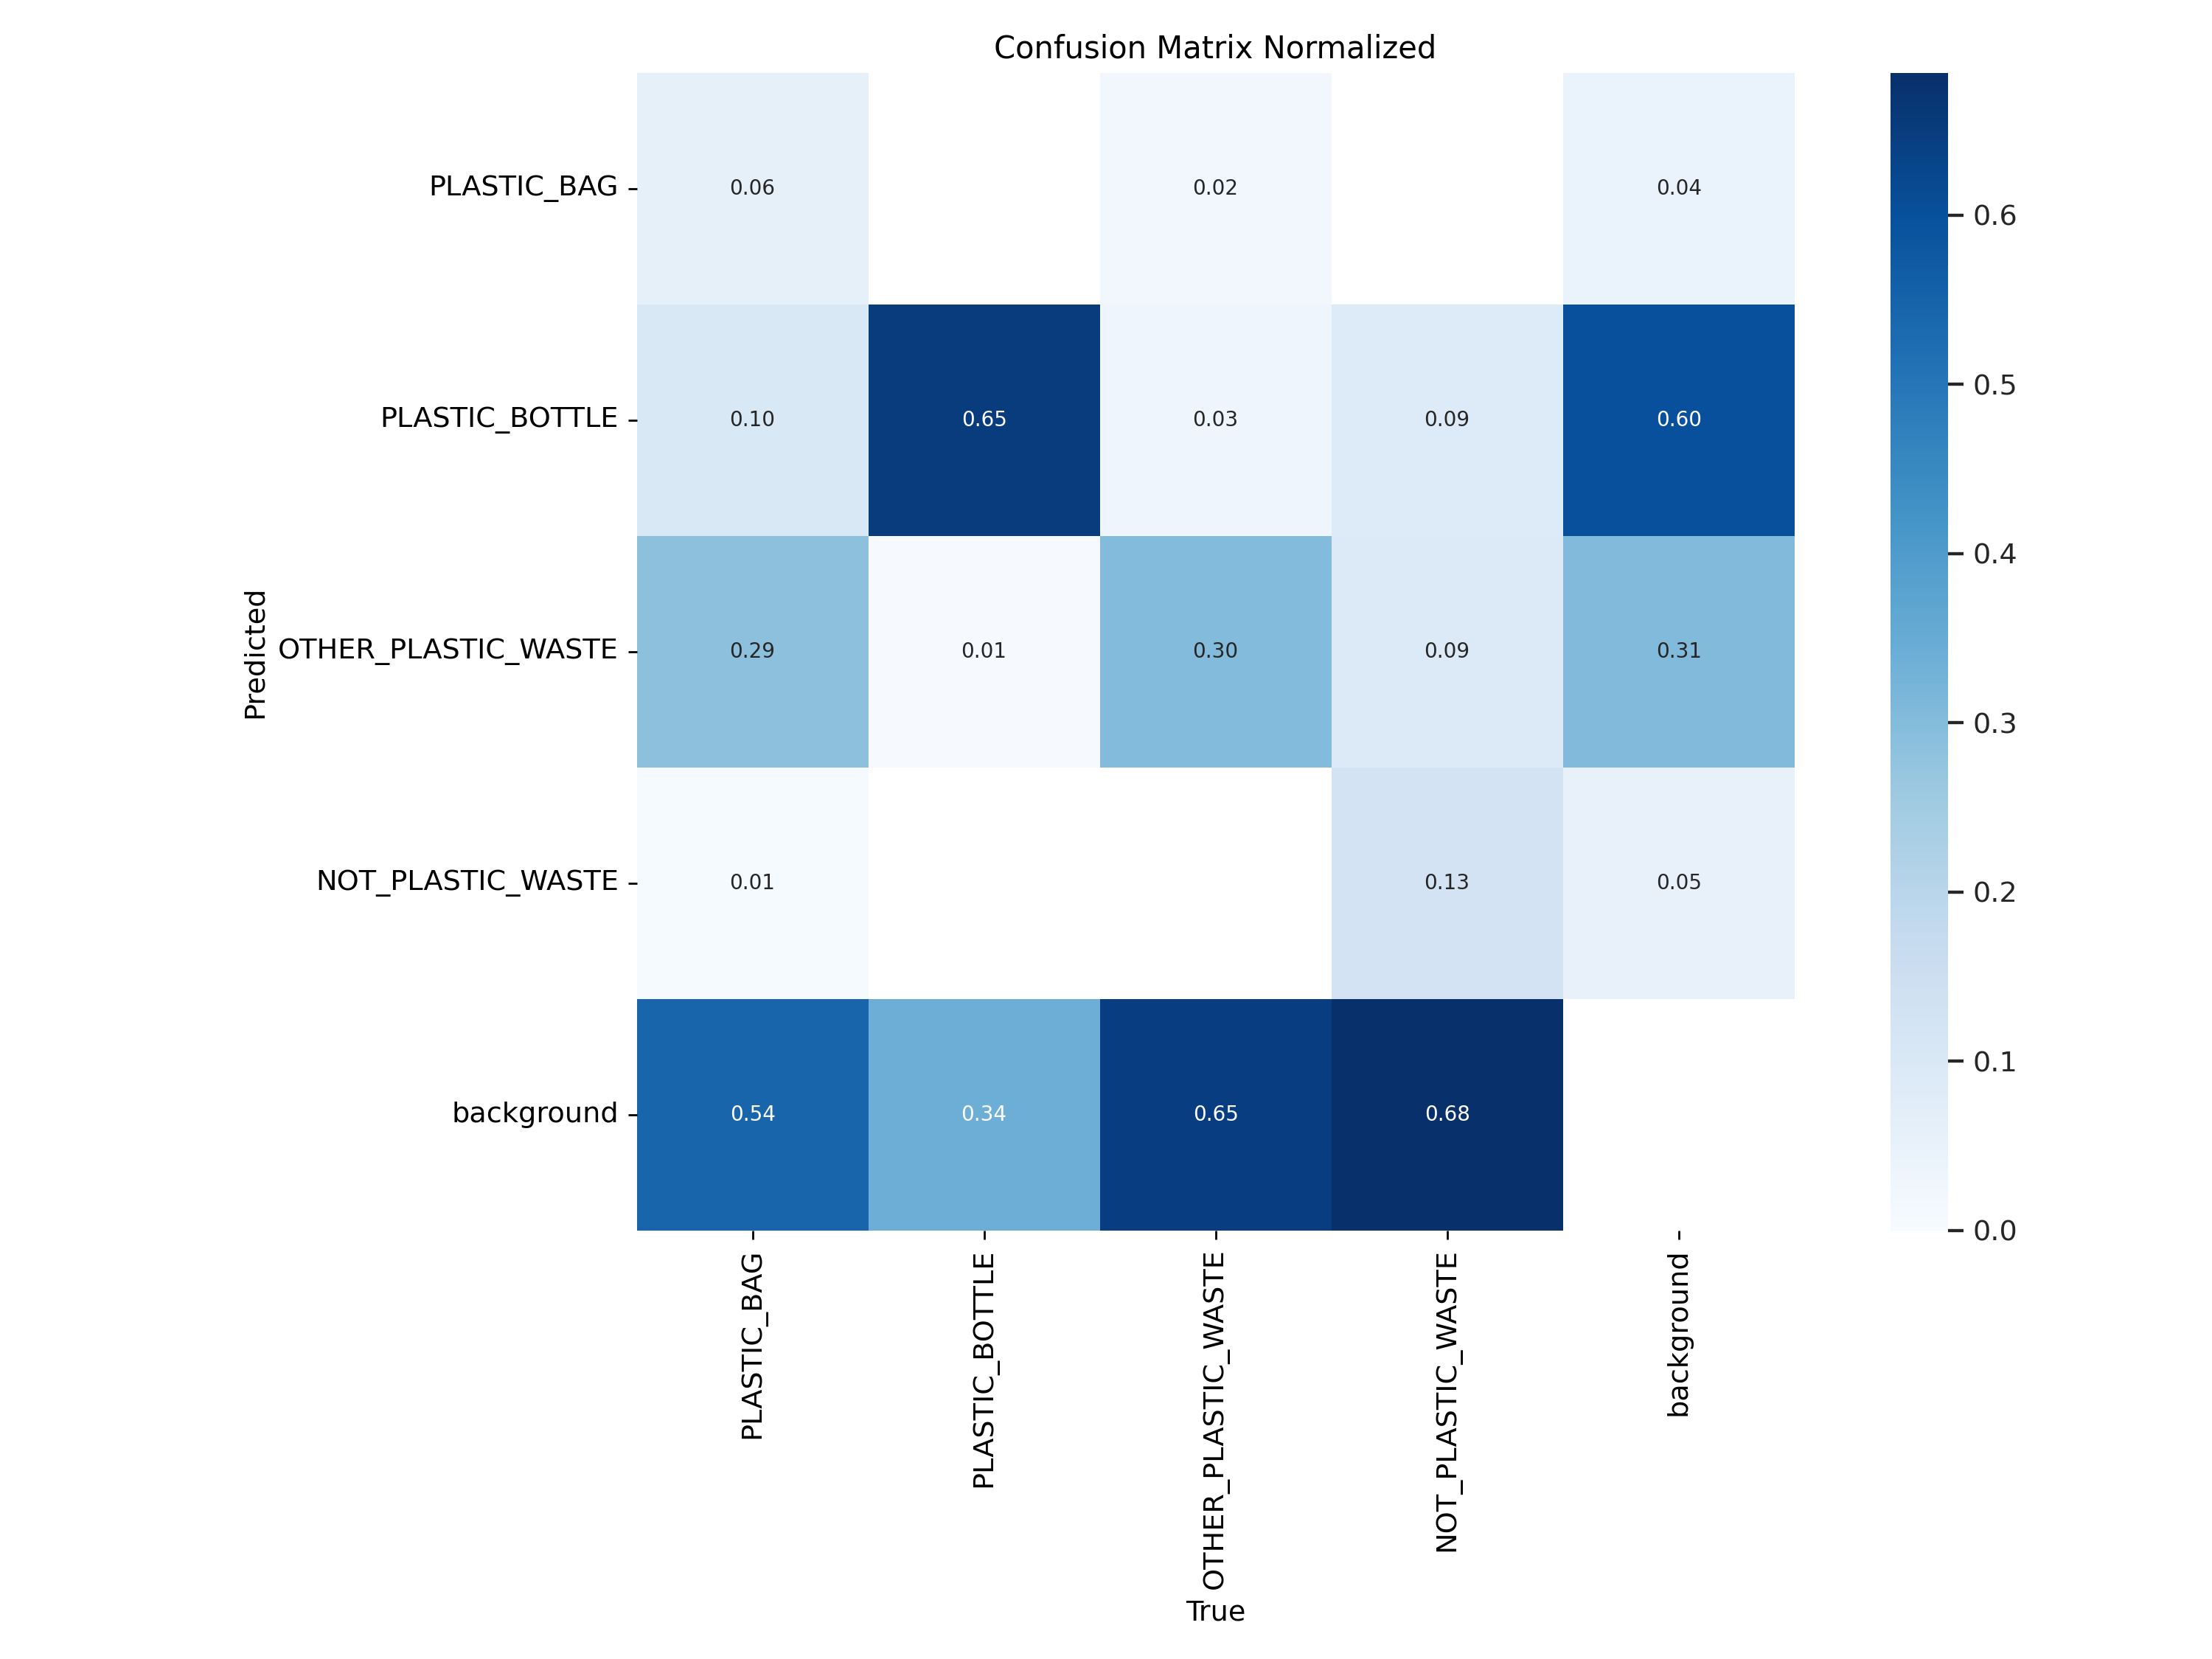
\includegraphics[width=0.8\textwidth]{v_2/small-1203/confusion_matrix_normalized.png}
    \caption{Matrice di confusione normalizzata data dal modello \texttt{small-1203}}
    \label{fig:v2-4}
\end{figure}

\subsection*{Modello 3 - medium-200-0}

% Introduzione su strategia del training -> qual è l'obiettivo dell'esperimento?

% Dettagli configurazione, tipologia modello e iperparametri, dove è stato eseguito il train

% Risultati training
    % - andamento training
    % - grafici recall e precision e performance e F1
    % - matrici di confusione
    % - tabella performance test set

% Commento risultati

primo modello

\subsection*{Modello 4 - small-tune-03 e small-tune-04}

% Introduzione su strategia del training -> qual è l'obiettivo dell'esperimento?

% Dettagli configurazione, tipologia modello e iperparametri, dove è stato eseguito il train

% Risultati training
    % - andamento training
    % - grafici recall e precision e performance e F1
    % - matrici di confusione
    % - tabella performance test set

% Commento risultati

primo modello

% \subsection*{Modelli 5 - small-ukra-0 e medium-ukra-0}

% Introduzione su strategia del training -> qual è l'obiettivo dell'esperimento?

Modelli con rifermento al paper trovato

Modelli addestrati su server serina

% Dettagli configurazione, tipologia modello e iperparametri, dove è stato eseguito il train

% Risultati training
    % - andamento training
    % - grafici recall e precision e performance e F1
    % - matrici di confusione
    % - tabella performance test set

% Commento risultati

primo modello
% \subsection*{Modelli 6 - tuning iperparametri}

L'ultimo esperimento rimasto è quello di effettuare una regolazione degli iperparametri tramite 
fine tuning. Abbiamo pertanto utilizzato lo strumento \texttt{tuner} della libreria ultralytics
per poter ricavare i valori migliori per gli iperparametri. Tale \texttt{tuner} effettua una serie 
di training con dei valori di iperparametri iniziali. Ogni iterazione consiste in una manciata
di epoche  di training necessarie per poter ottenere un modello da valutare. Alla fine di ogni 
iterazione si valuta tale modello in relazione ai suoi iperparametri. Con la nuova iterazione 
gli iperparametri vengono impostati a dei nuovi valori che vengono stabiliti dall'algoritmo del
\texttt{tuner}. L'evoluzione degli iperparametri segue un algoritmo genetico in modo da poter 
indirizzare i valori verso le prestazioni migliori.

Per far si che potessimo ottenere dei risultati consistenti anche dopo la fase di training, 
abbiamo effettuato la fase di tuning con il validation set in modo che successivamente i 
risultati non fossero influenzati da un overfitting degli iperparametri su training set.
La successiva fase di addestramento ha visto l'uso normale dei sottoinsiemi del dataset per 
train, validazione e test.

La fase di tuning è stata quella che ha richiesto più risorse, sia in termini di tempo che di 
potenza di calcolo. Nella figura \ref{fig:v6-1} è possibile vedere l'andamento della funzione 
di fitness, funzione che valutava la bontà degli iperparametri utilizzati, mentre nella figura 
\ref{fig:v6-2} l'andamento dei valori degli iperparametri nel corso del tuning.

\begin{figure}[!htb]
    \centering
    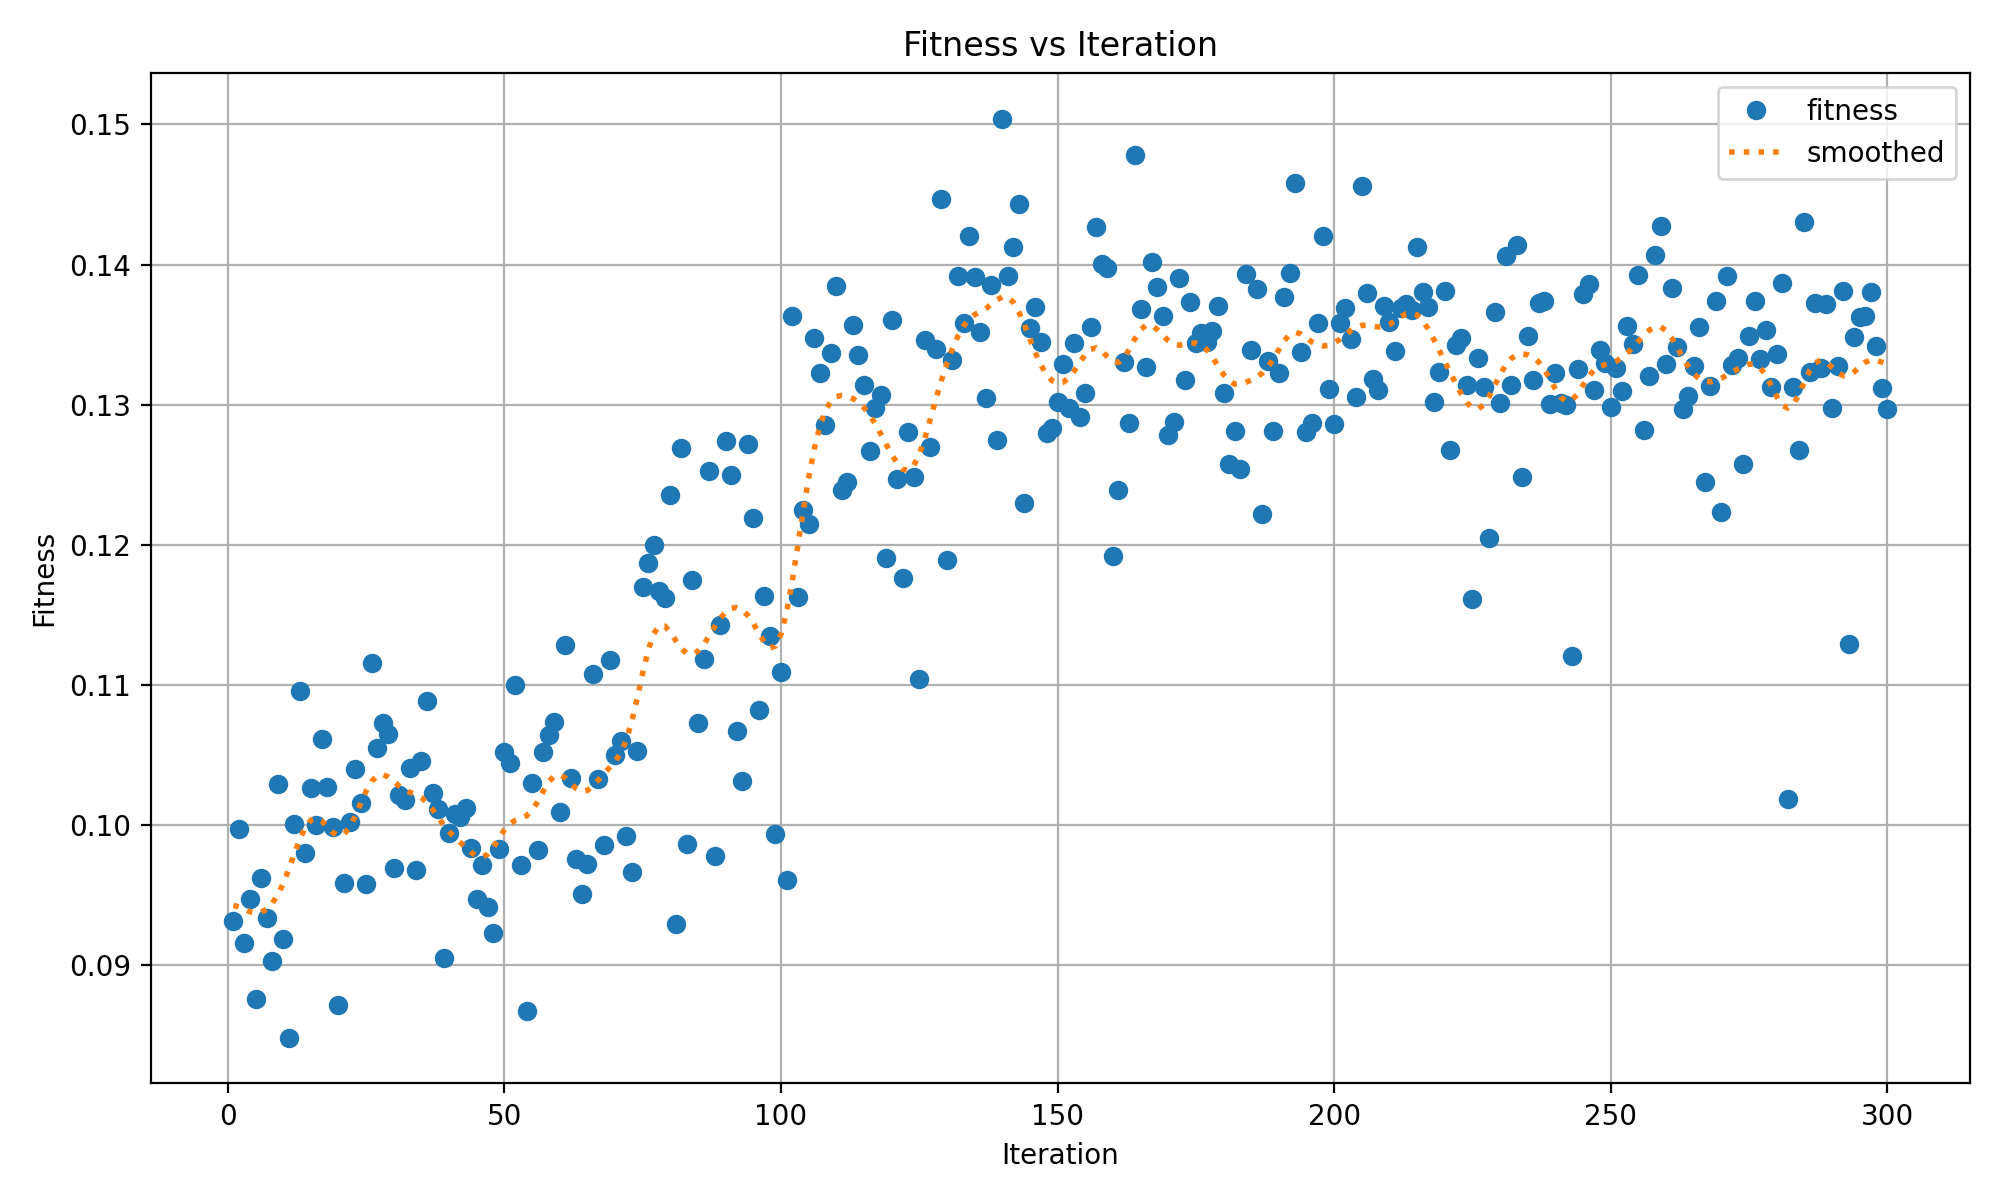
\includegraphics[width=0.8\textwidth]{v_6/tune/tune_fitness.png}
    \caption{Andamento funzioni di fitness durante l'esecuzione del tuning degli iperparametri}
    \label{fig:v6-1}
\end{figure}

\begin{figure}[!htb]
    \centering
    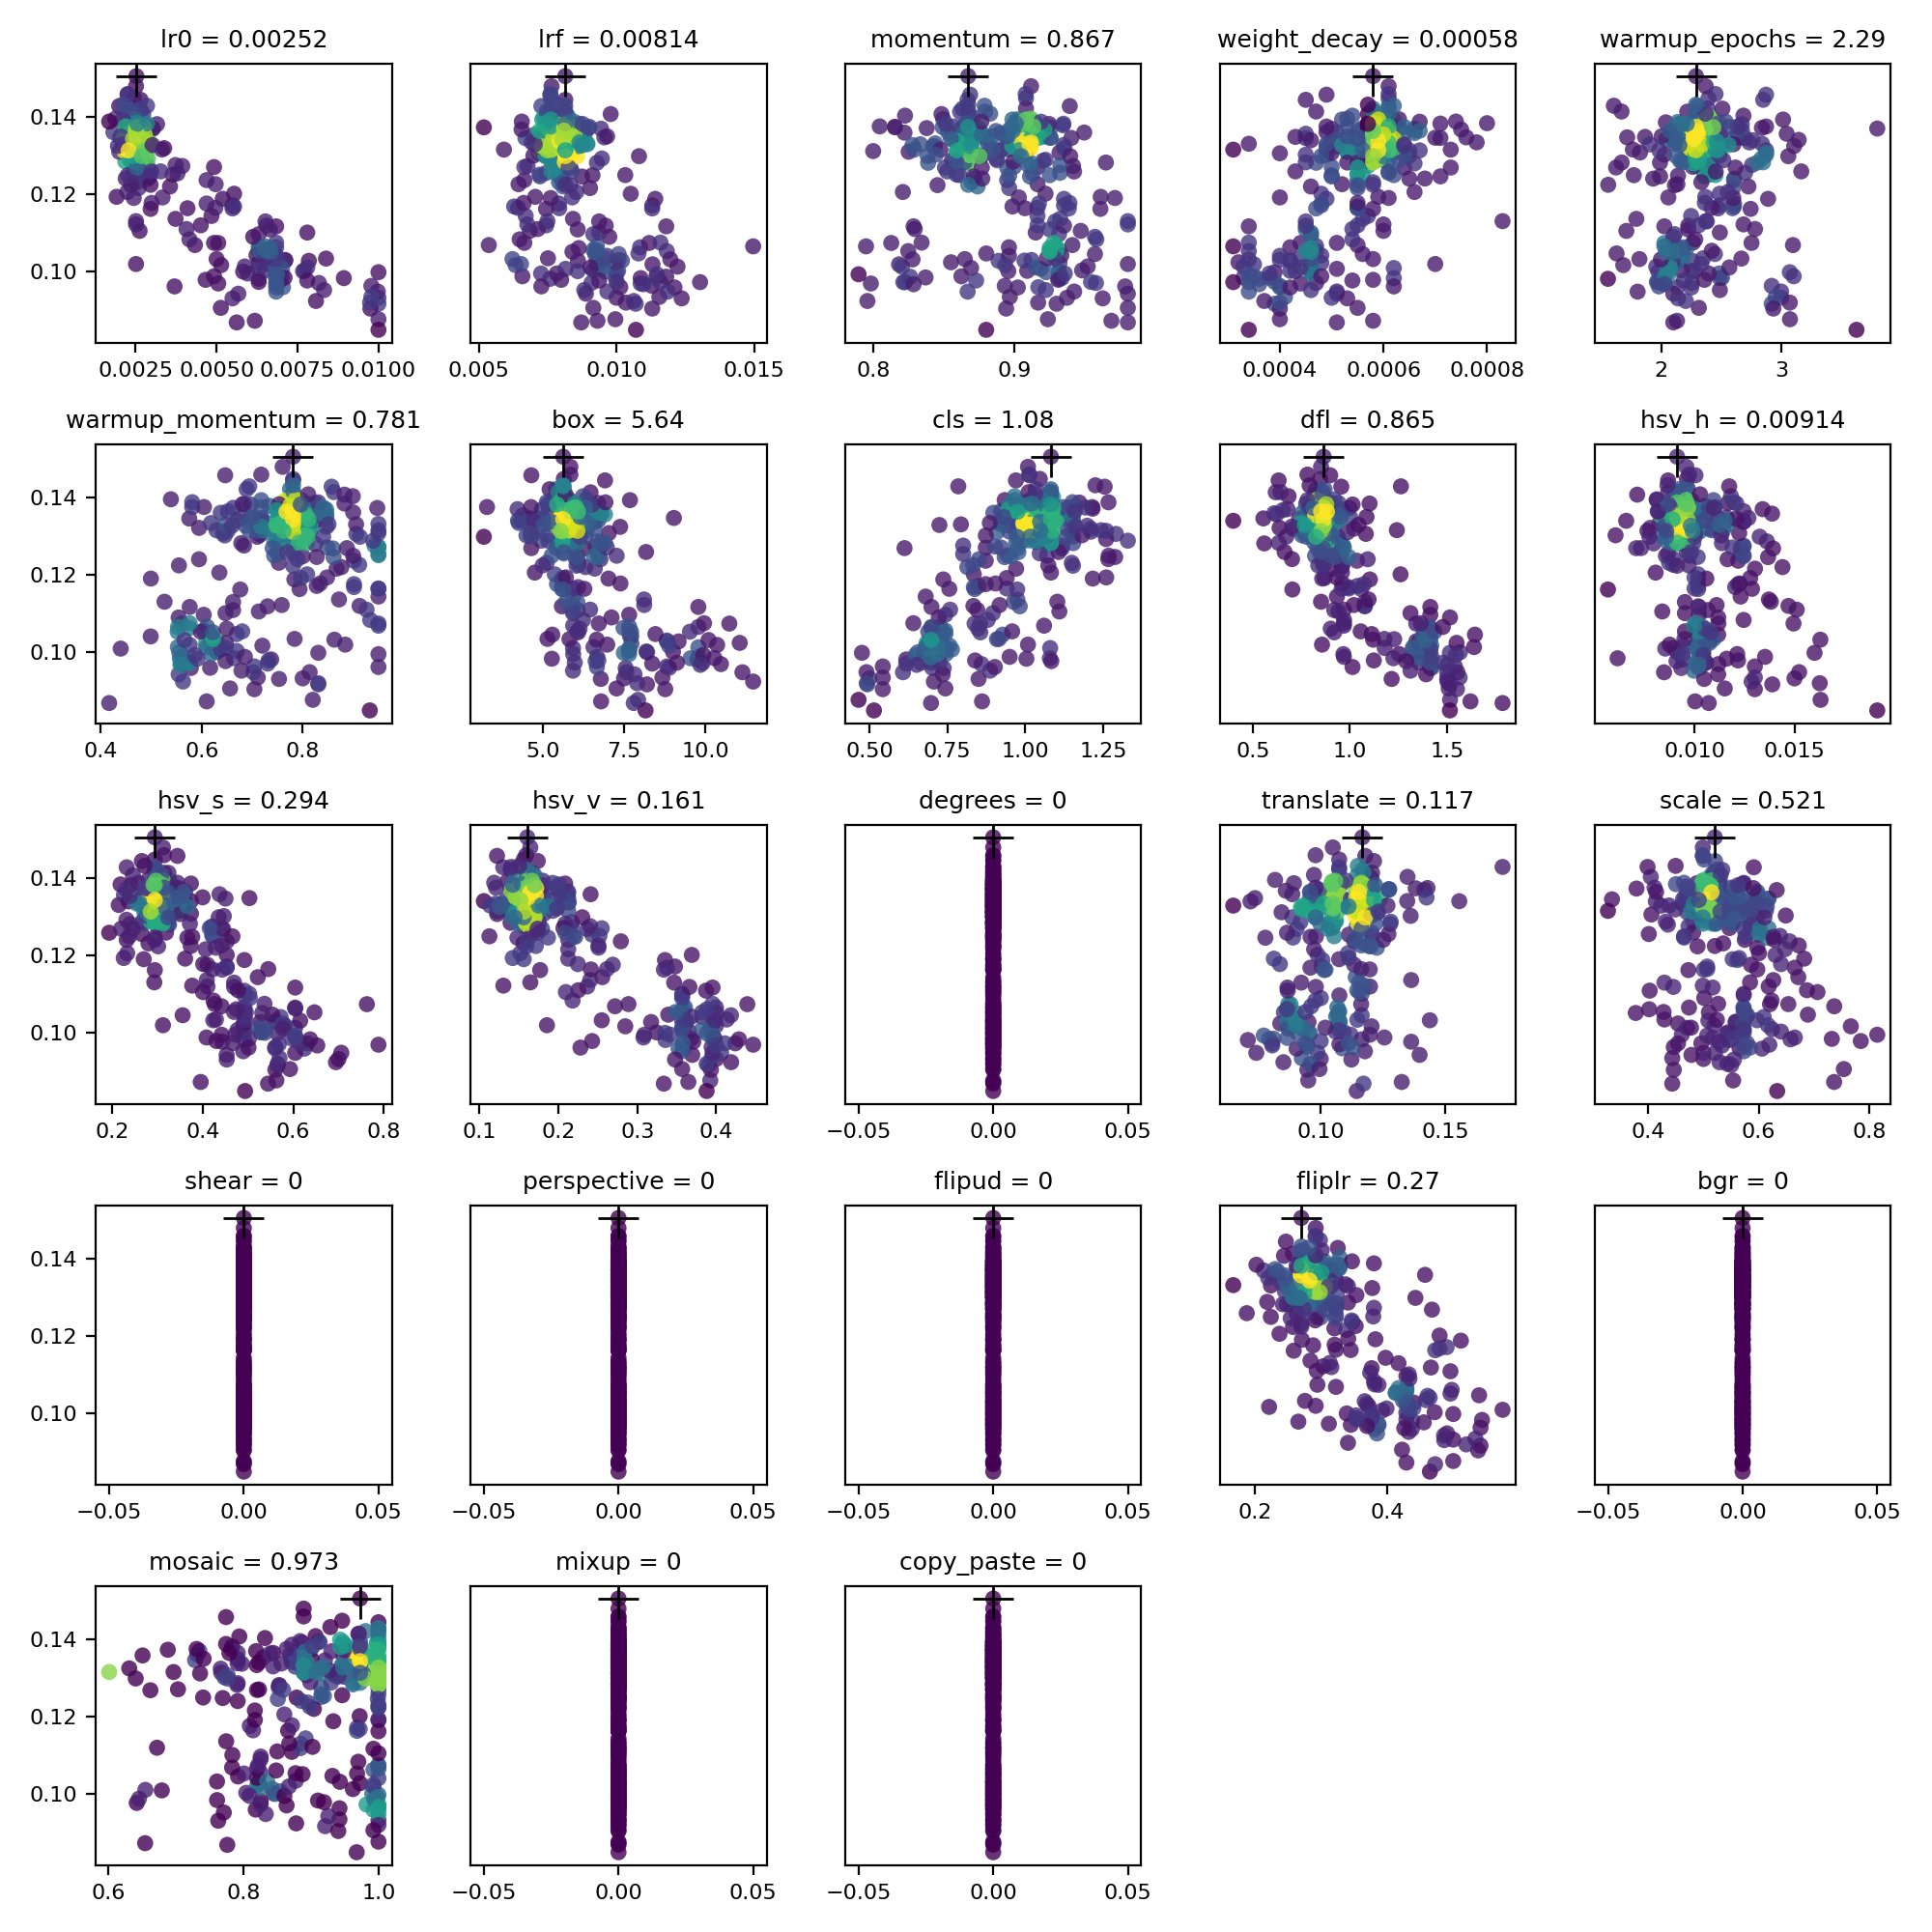
\includegraphics[width=0.8\textwidth]{v_6/tune/tune_scatter_plots.png}
    \caption{Andamento valori degli iperparametri durante la fase di tuning}
    \label{fig:v6-2}
\end{figure}

Questa fase ha visto l'utilizzo del modello nano di YOLO, YOLOv8n, per 300 iterazioni ciascuna da 
30 epoche di addestramento. Gli iperparametri migliori, poi utilizzati nella fase di training, sono 
elencati nella tabella \ref*{table:v6-1}.

\begin{table}[!htbp]
    \centering
    \begin{tabularx}{\textwidth}{lYYY}
        \toprule
        \textbf{Iperparametro} & \textbf{Valori risultati dal Tuning} & \textbf{Valore Predefinito} & \textbf{Descrizione} \\
        \midrule
        \texttt{lr0} & 0.00252 & 0.01 & Learning rate iniziale \\
        \texttt{lrf} & 0.00814 & 0.01 & Learning rate finale \\
        \texttt{momentum} & 0.86722 & 0.937 & Fattore di momentum \\
        \texttt{weight\_decay} & 0.00058 & 0.0005 & Termine di regolarizzazione per i pesi \\
        \texttt{warmup\_epochs} & 2.28985 & 3.0 & Numero di epoche di warmup \\
        \texttt{warmup\_momentum} & 0.78103 & 0.8 & Momentum iniziale durante il warmup \\
        \texttt{box} & 5.6359 & 0.05 & Guadagno della loss per il box \\
        \texttt{cls} & 1.08241 & 0.5 & Guadagno della loss per la classificazione \\
        \texttt{dfl} & 0.86478 & 1.5 & Guadagno della Distribution Focal Loss \\
        \texttt{hsv\_h} & 0.00914 & 0.015 & Fattore di aumento della tonalità \\
        \texttt{hsv\_s} & 0.29432 & 0.7 & Fattore di aumento della saturazione \\
        \texttt{hsv\_v} & 0.16061 & 0.4 & Fattore di aumento del valore \\
        \texttt{translate} & 0.11669 & 0.1 & Fattore di traslazione dell'immagine \\
        \texttt{scale} & 0.52052 & 0.5 & Fattore di scala dell'immagine \\
        \texttt{fliplr} & 0.27039 & 0.5 & Probabilità di ribaltamento orizzontale \\
        \texttt{mosaic} & 0.9728 & 1.0 & Fattore di aumento mosaic \\
        \bottomrule
    \end{tabularx}
    \caption{Risultati della sintonizzazione degli iperparametri di YOLOv8}
    \label{table:v6-1}
\end{table}

Questa configurazione è stata utilizzata per l'esecuzione di 3 addestramenti, per i modelli
\texttt{nano}, \texttt{small} e \texttt{medium} di YOLO. Ogni training ha avuto a disposizione
500 epoche con 200 epoche di \texttt{patience} prima di procedere con l'early stopping. 
\texttt{imgsz} è rimasto impostato a 800 pixel mentre come ottimizzatore è stato utilizzato AdamW.
Il nome dato ai modelli per questi training è \textit{size}\texttt{-tune-2.0}.

\begin{figure}[!htb]
    \centering
    \begin{subfigure}{.8\textwidth}
        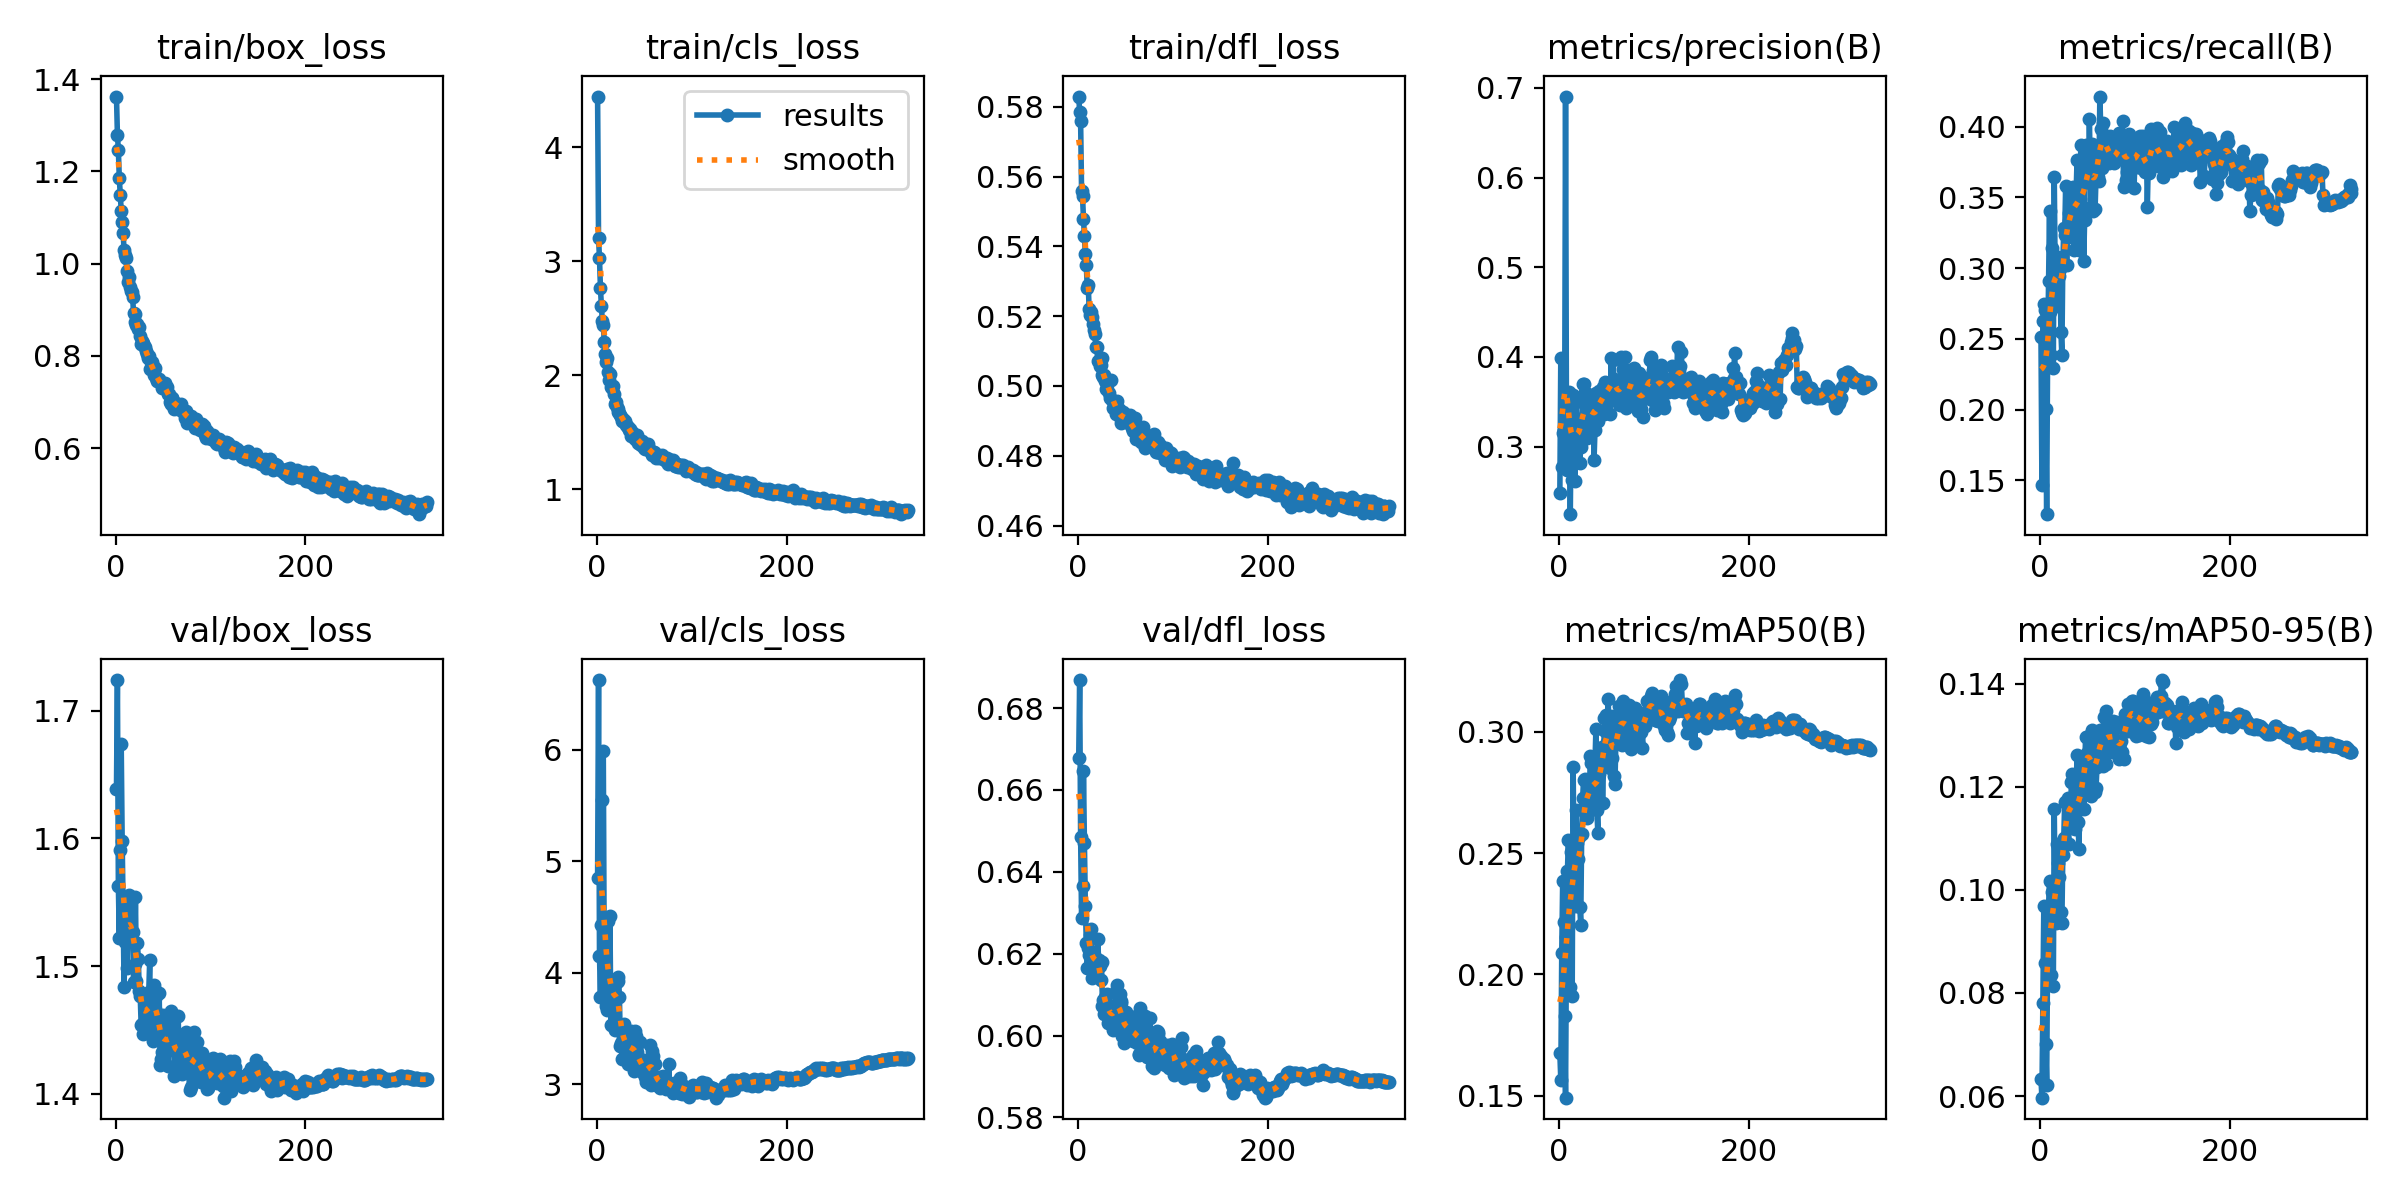
\includegraphics[width=0.9\textwidth]{v_6/nano-tune-2.0/results.png}
        \subcaption{Nano}
        \label{fig:v6-3.1}
    \end{subfigure}
    \begin{subfigure}{.8\textwidth}
        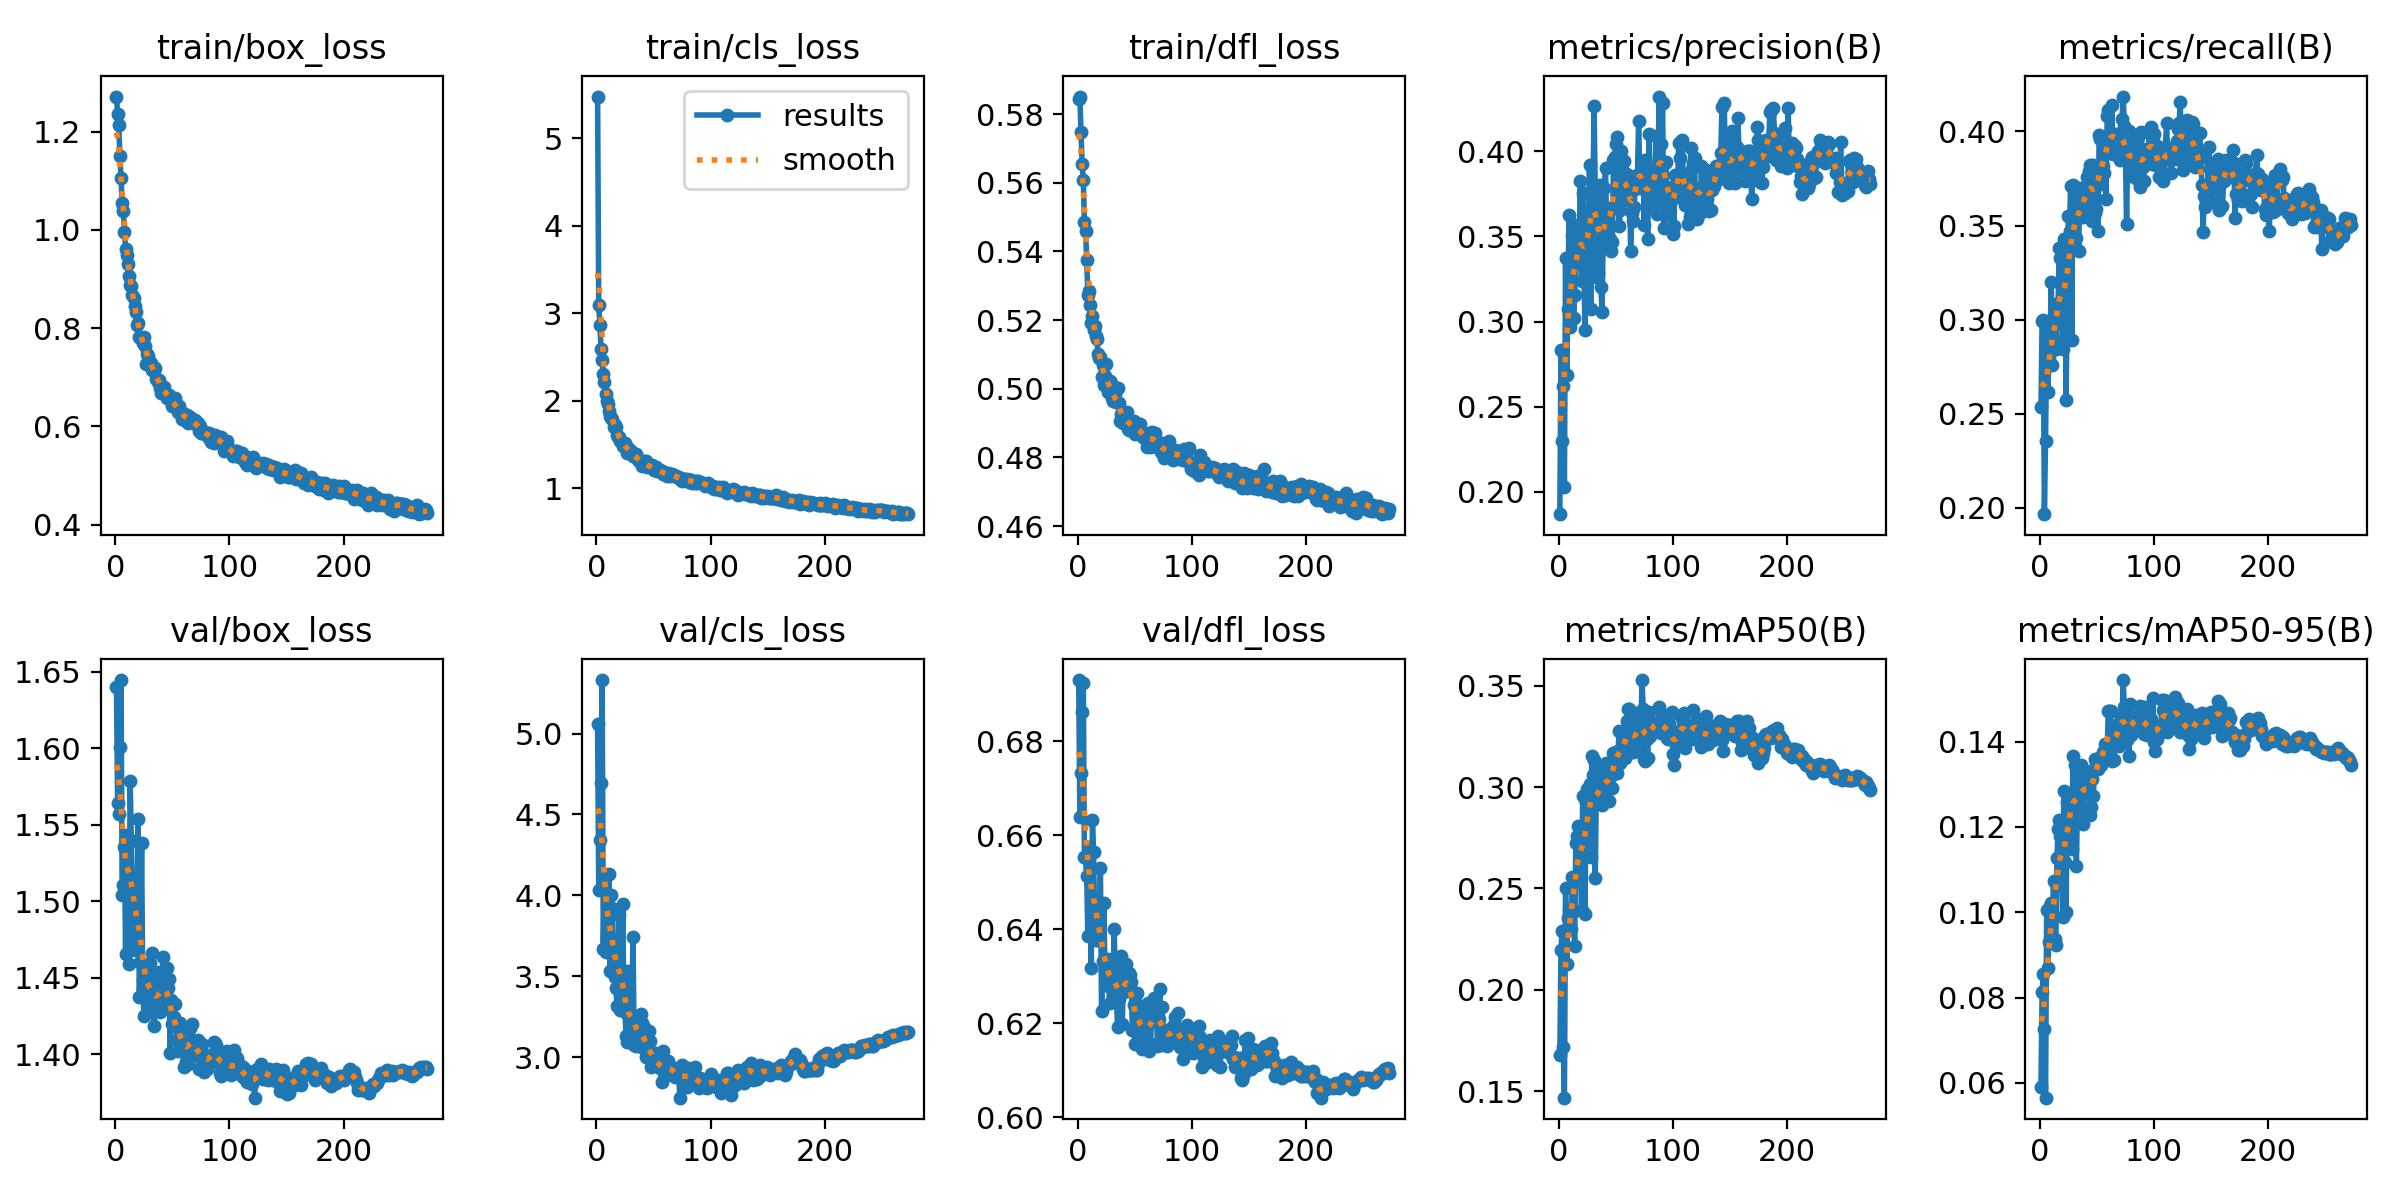
\includegraphics[width=0.9\textwidth]{v_6/small-tune-2.0/results.png}
        \subcaption{Small}
        \label{fig:v6-3.2}
    \end{subfigure}
    \begin{subfigure}{.8\textwidth}
        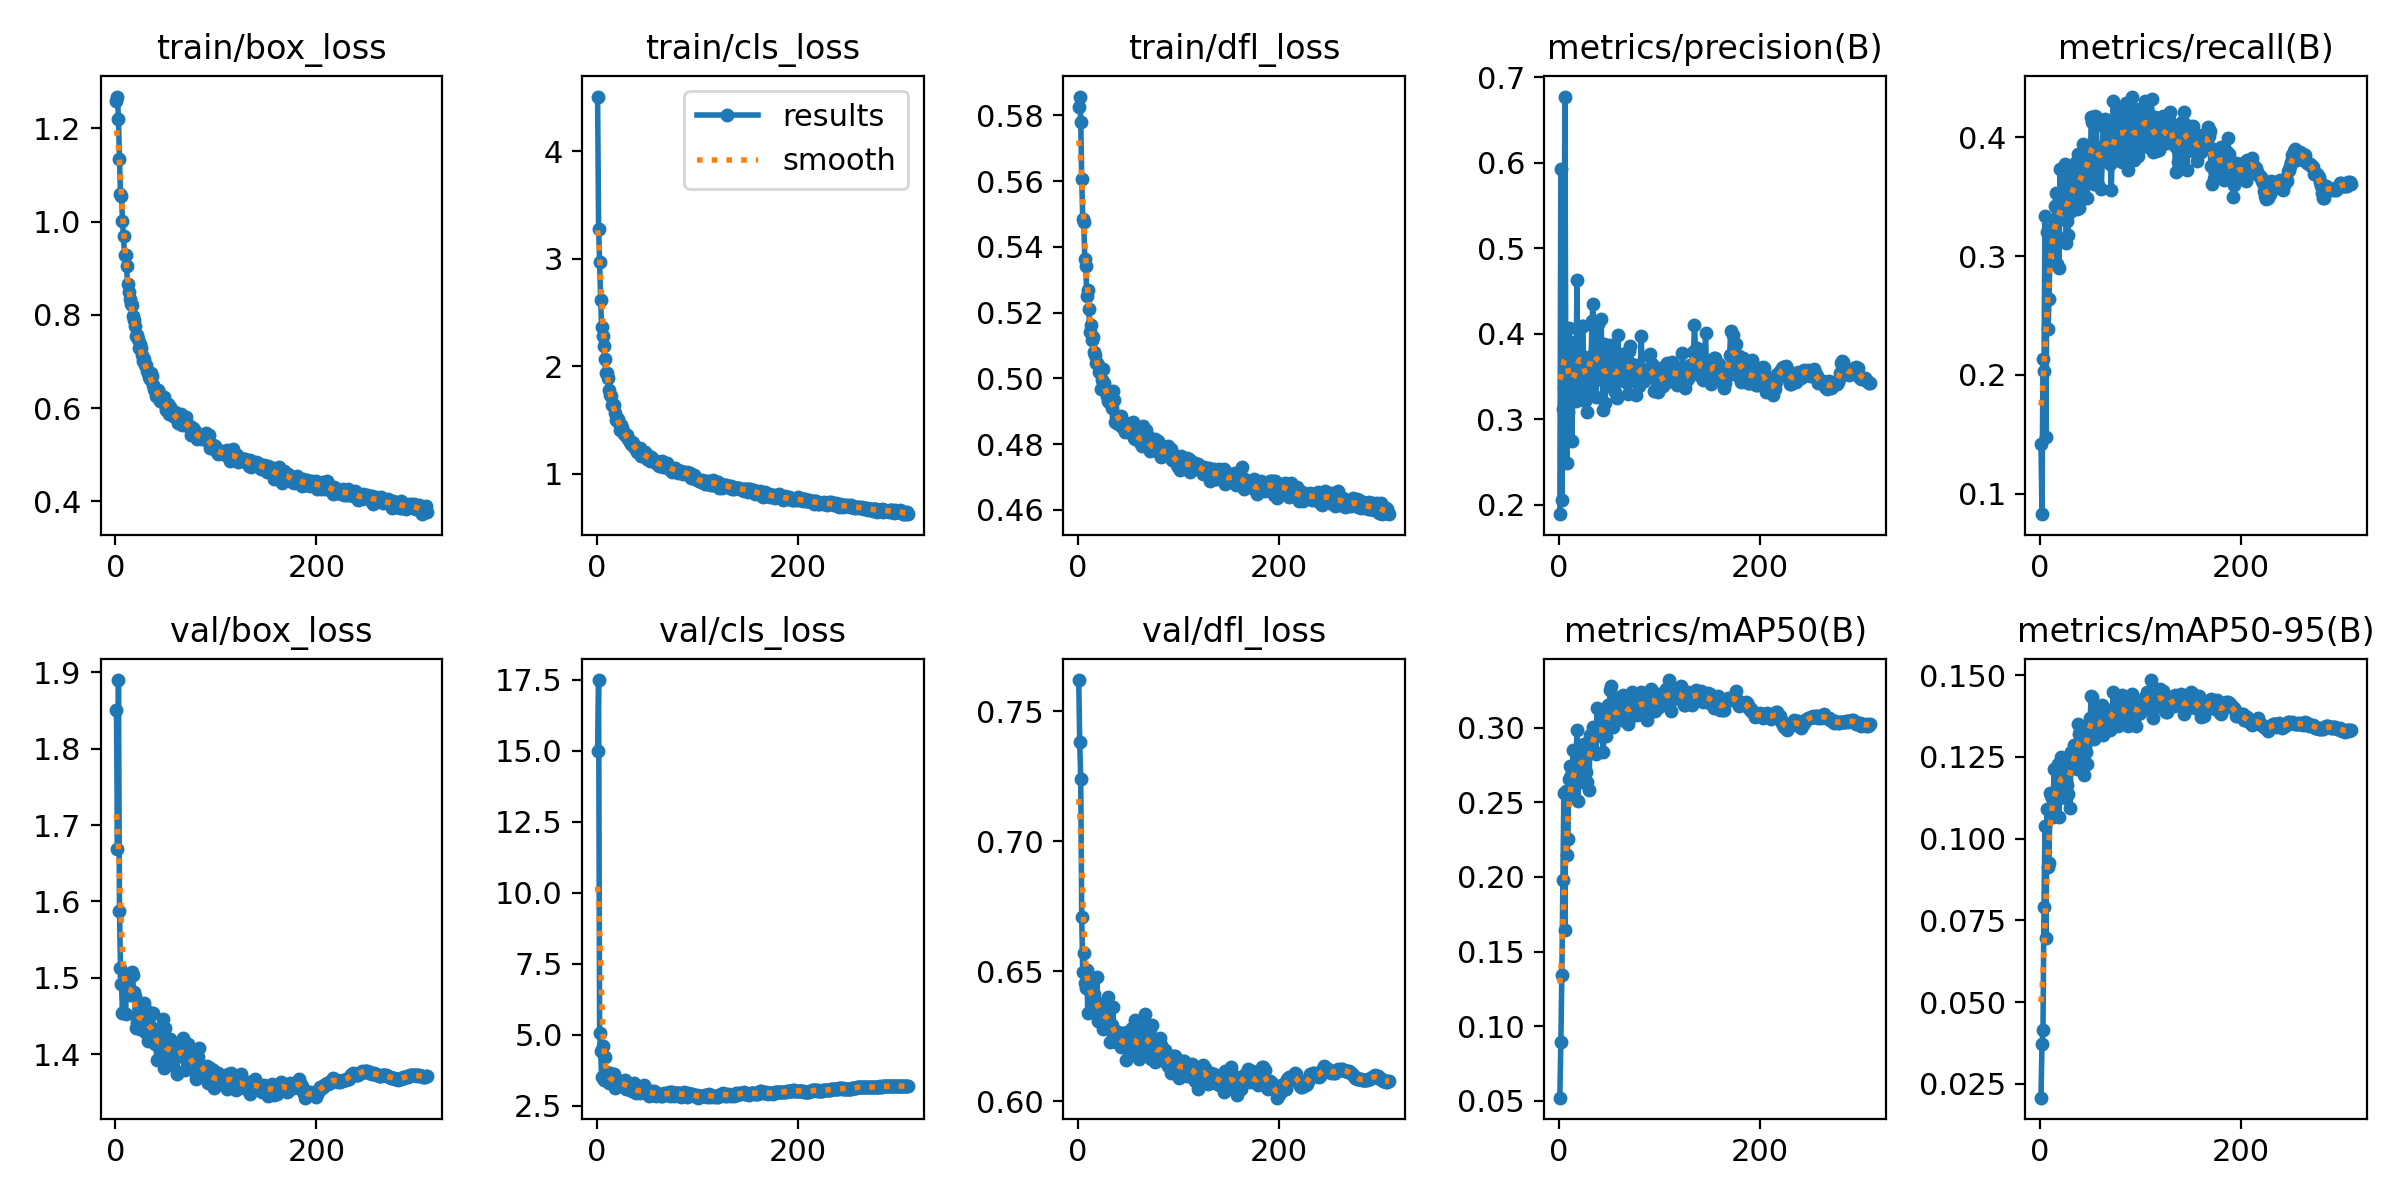
\includegraphics[width=0.9\textwidth]{v_6/medium-tune-2.0/results.png}
        \subcaption{Medium}
        \label{fig:v6-3.3}
    \end{subfigure}
    \caption{Comparazione tra l'andamento delle funzioni di errore durante il training
    dei modelli \textit{size}\texttt{-tune-2.0}}
    \label{fig:v6-3}
\end{figure}

\begin{table}[!htb]
    \centering
    \begin{tabularx}{\textwidth}{lYYYc}
        \toprule
        Class & P & R & mAP50 & mAP50-95 \\
        \midrule
        \texttt{nano-tune-2.0} \\
        \midrule
        ALL & 0.372 & 0.428 & 0.320 & 0.159 \\
        PLASTIC\_BAG & 0.223 & 0.329 & 0.158 & 0.0463 \\
        PLASTIC\_BOTTLE & 0.714 & 0.737 & 0.751 & 0.385 \\
        OTHER\_PLASTIC\_WASTE & 0.141 & 0.385 & 0.103 & 0.0319 \\
        NOT\_PLASTIC\_WASTE & 0.409 & 0.261 & 0.268 & 0.174 \\
        \midrule
        \texttt{small-tune-2.0} \\
        \midrule
        ALL & 0.400 & 0.389 & 0.345 & 0.172 \\
        PLASTIC\_BAG & 0.273 & 0.188 & 0.205 & 0.0662 \\
        PLASTIC\_BOTTLE & 0.741 & 0.724 & 0.757 & 0.395 \\
        OTHER\_PLASTIC\_WASTE & 0.152 & 0.293 & 0.0948 & 0.0297 \\
        NOT\_PLASTIC\_WASTE & 0.433 & 0.351 & 0.321 & 0.198 \\
        \midrule
        \texttt{medium-tune-2.0} \\
        \midrule
        ALL & 0.363 & 0.487 & 0.335 & 0.166 \\
        PLASTIC\_BAG & 0.254 & 0.372 & 0.194 & 0.0628 \\
        PLASTIC\_BOTTLE & 0.737 & 0.768 & 0.769 & 0.397 \\
        OTHER\_PLASTIC\_WASTE & 0.111 & 0.475 & 0.0952 & 0.0303 \\
        NOT\_PLASTIC\_WASTE & 0.350 & 0.334 & 0.280 & 0.173 \\
        \bottomrule
    \end{tabularx}
    \caption{Risultati delle metriche sul test set per \textit{size}\texttt{-tune-2.0}}
    \label{table:v6-2}
\end{table}

\begin{figure}[!htb]
    \centering
    \begin{subfigure}{.5\textwidth}
        \centering
        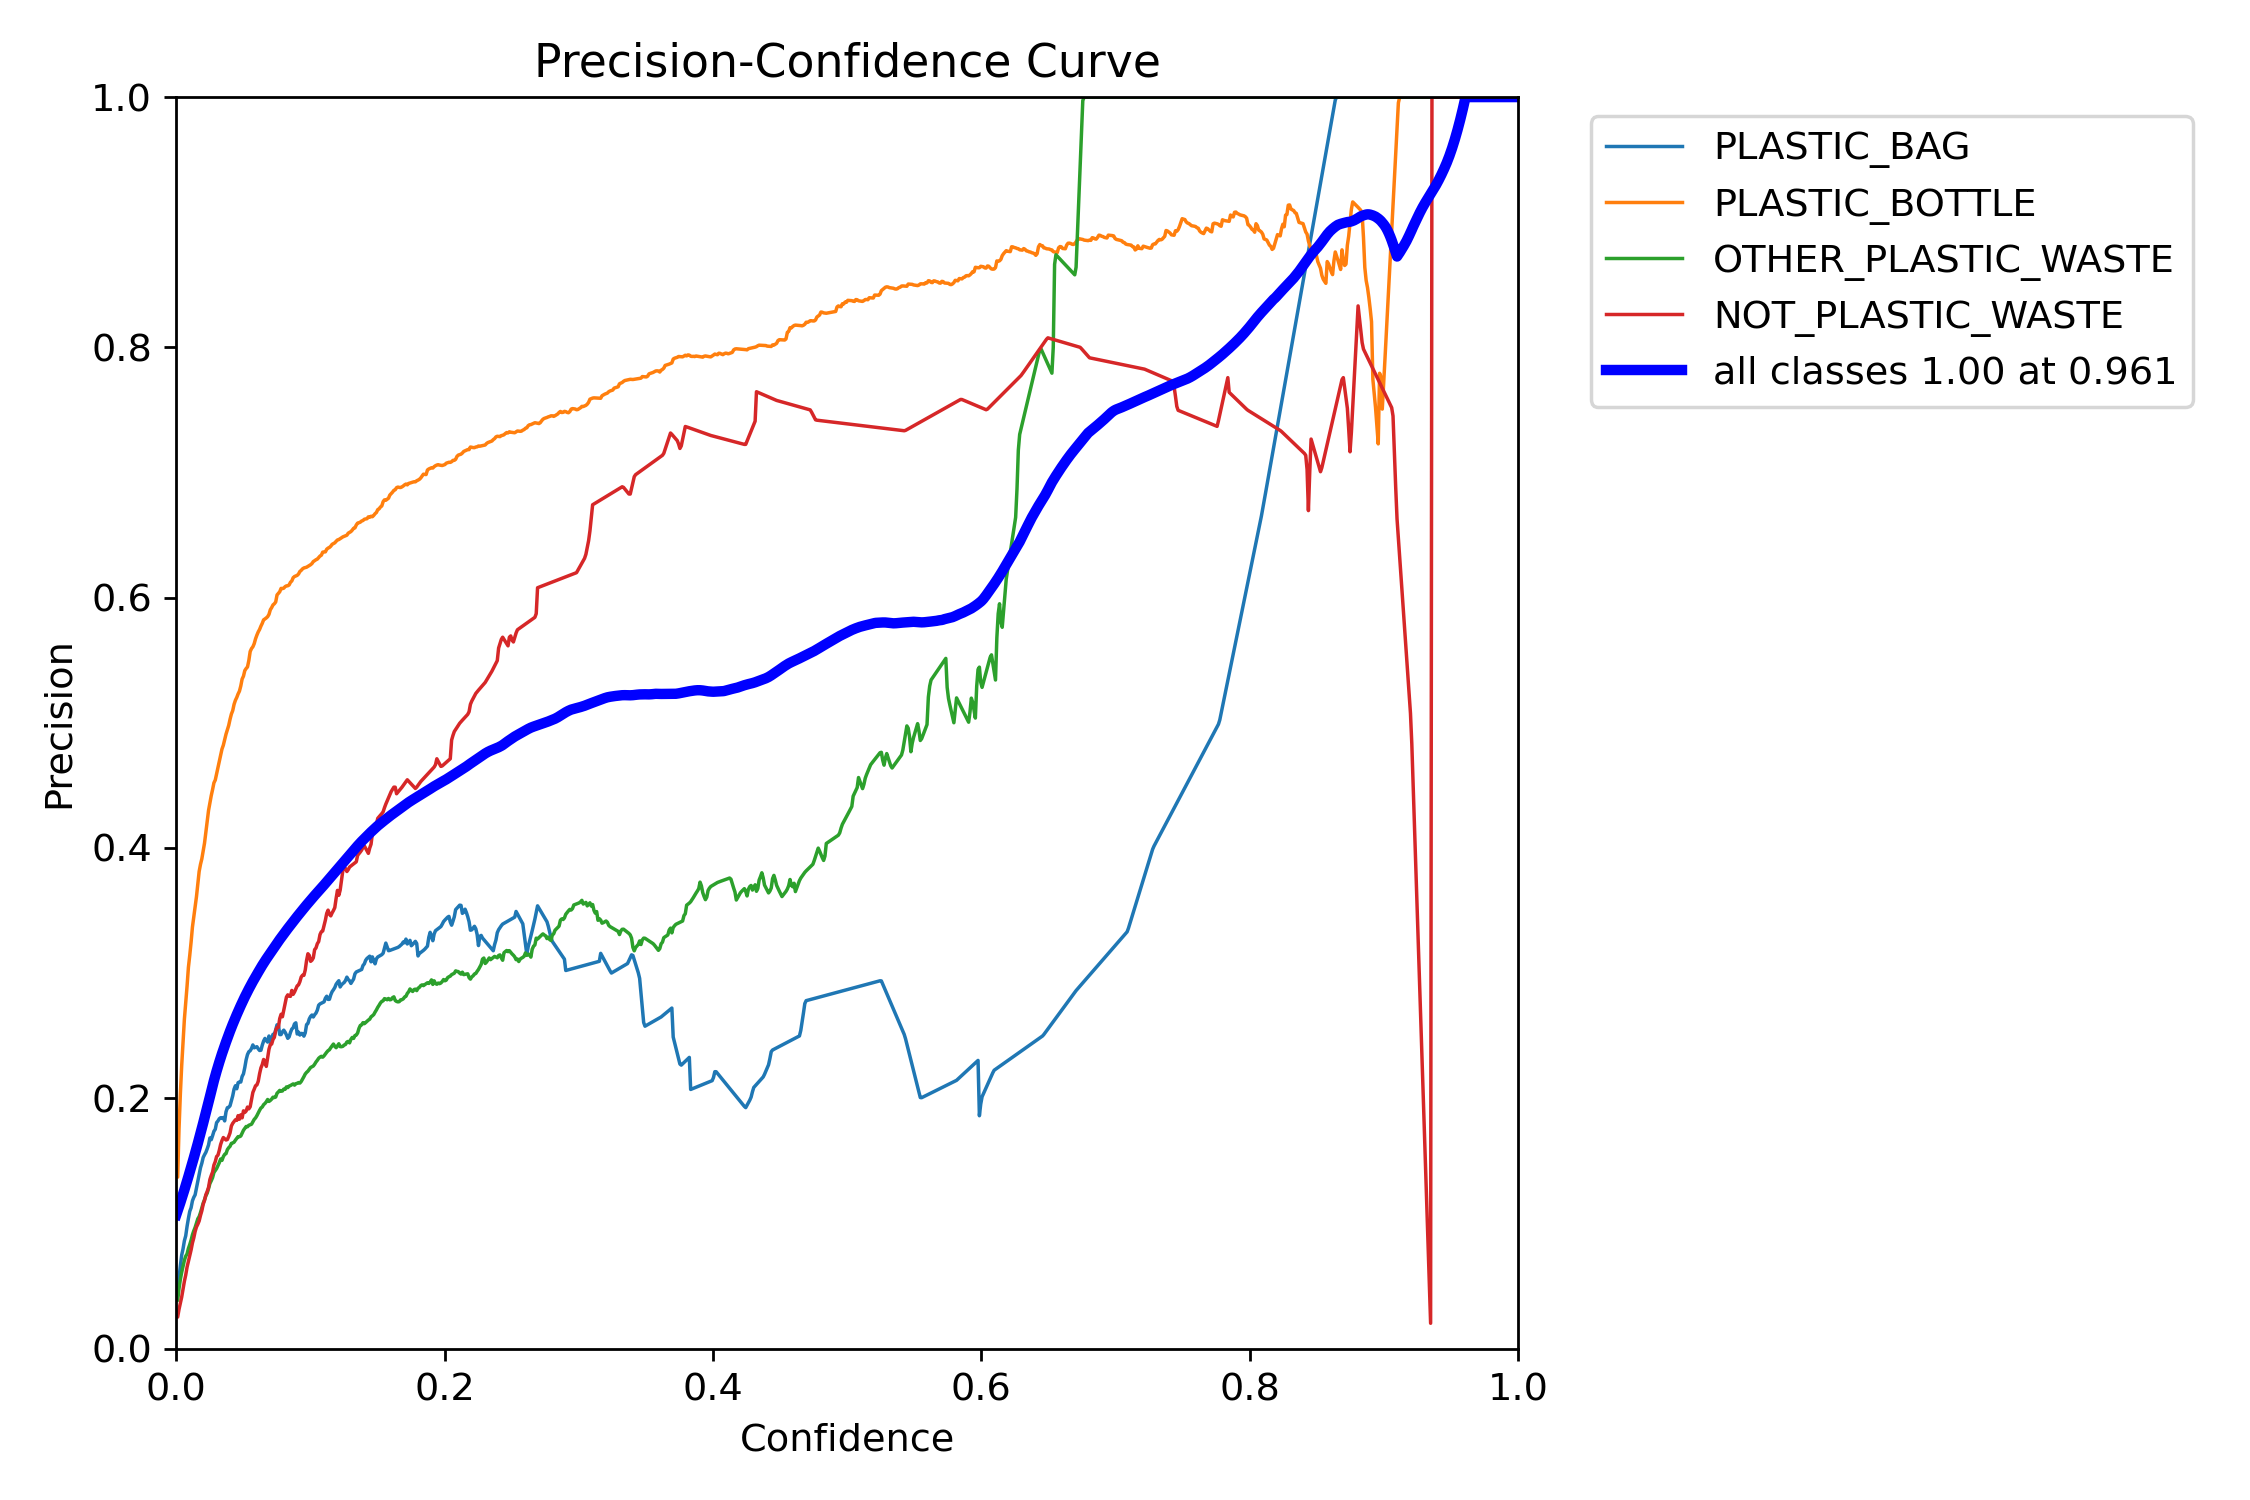
\includegraphics[width=.9\linewidth]{v_6/nano-tune-2.0/P_curve.png}
        \subcaption{P-curve}
        \label{fig:v6-4.1}
    \end{subfigure}%
      \begin{subfigure}{.5\textwidth}
        \centering
        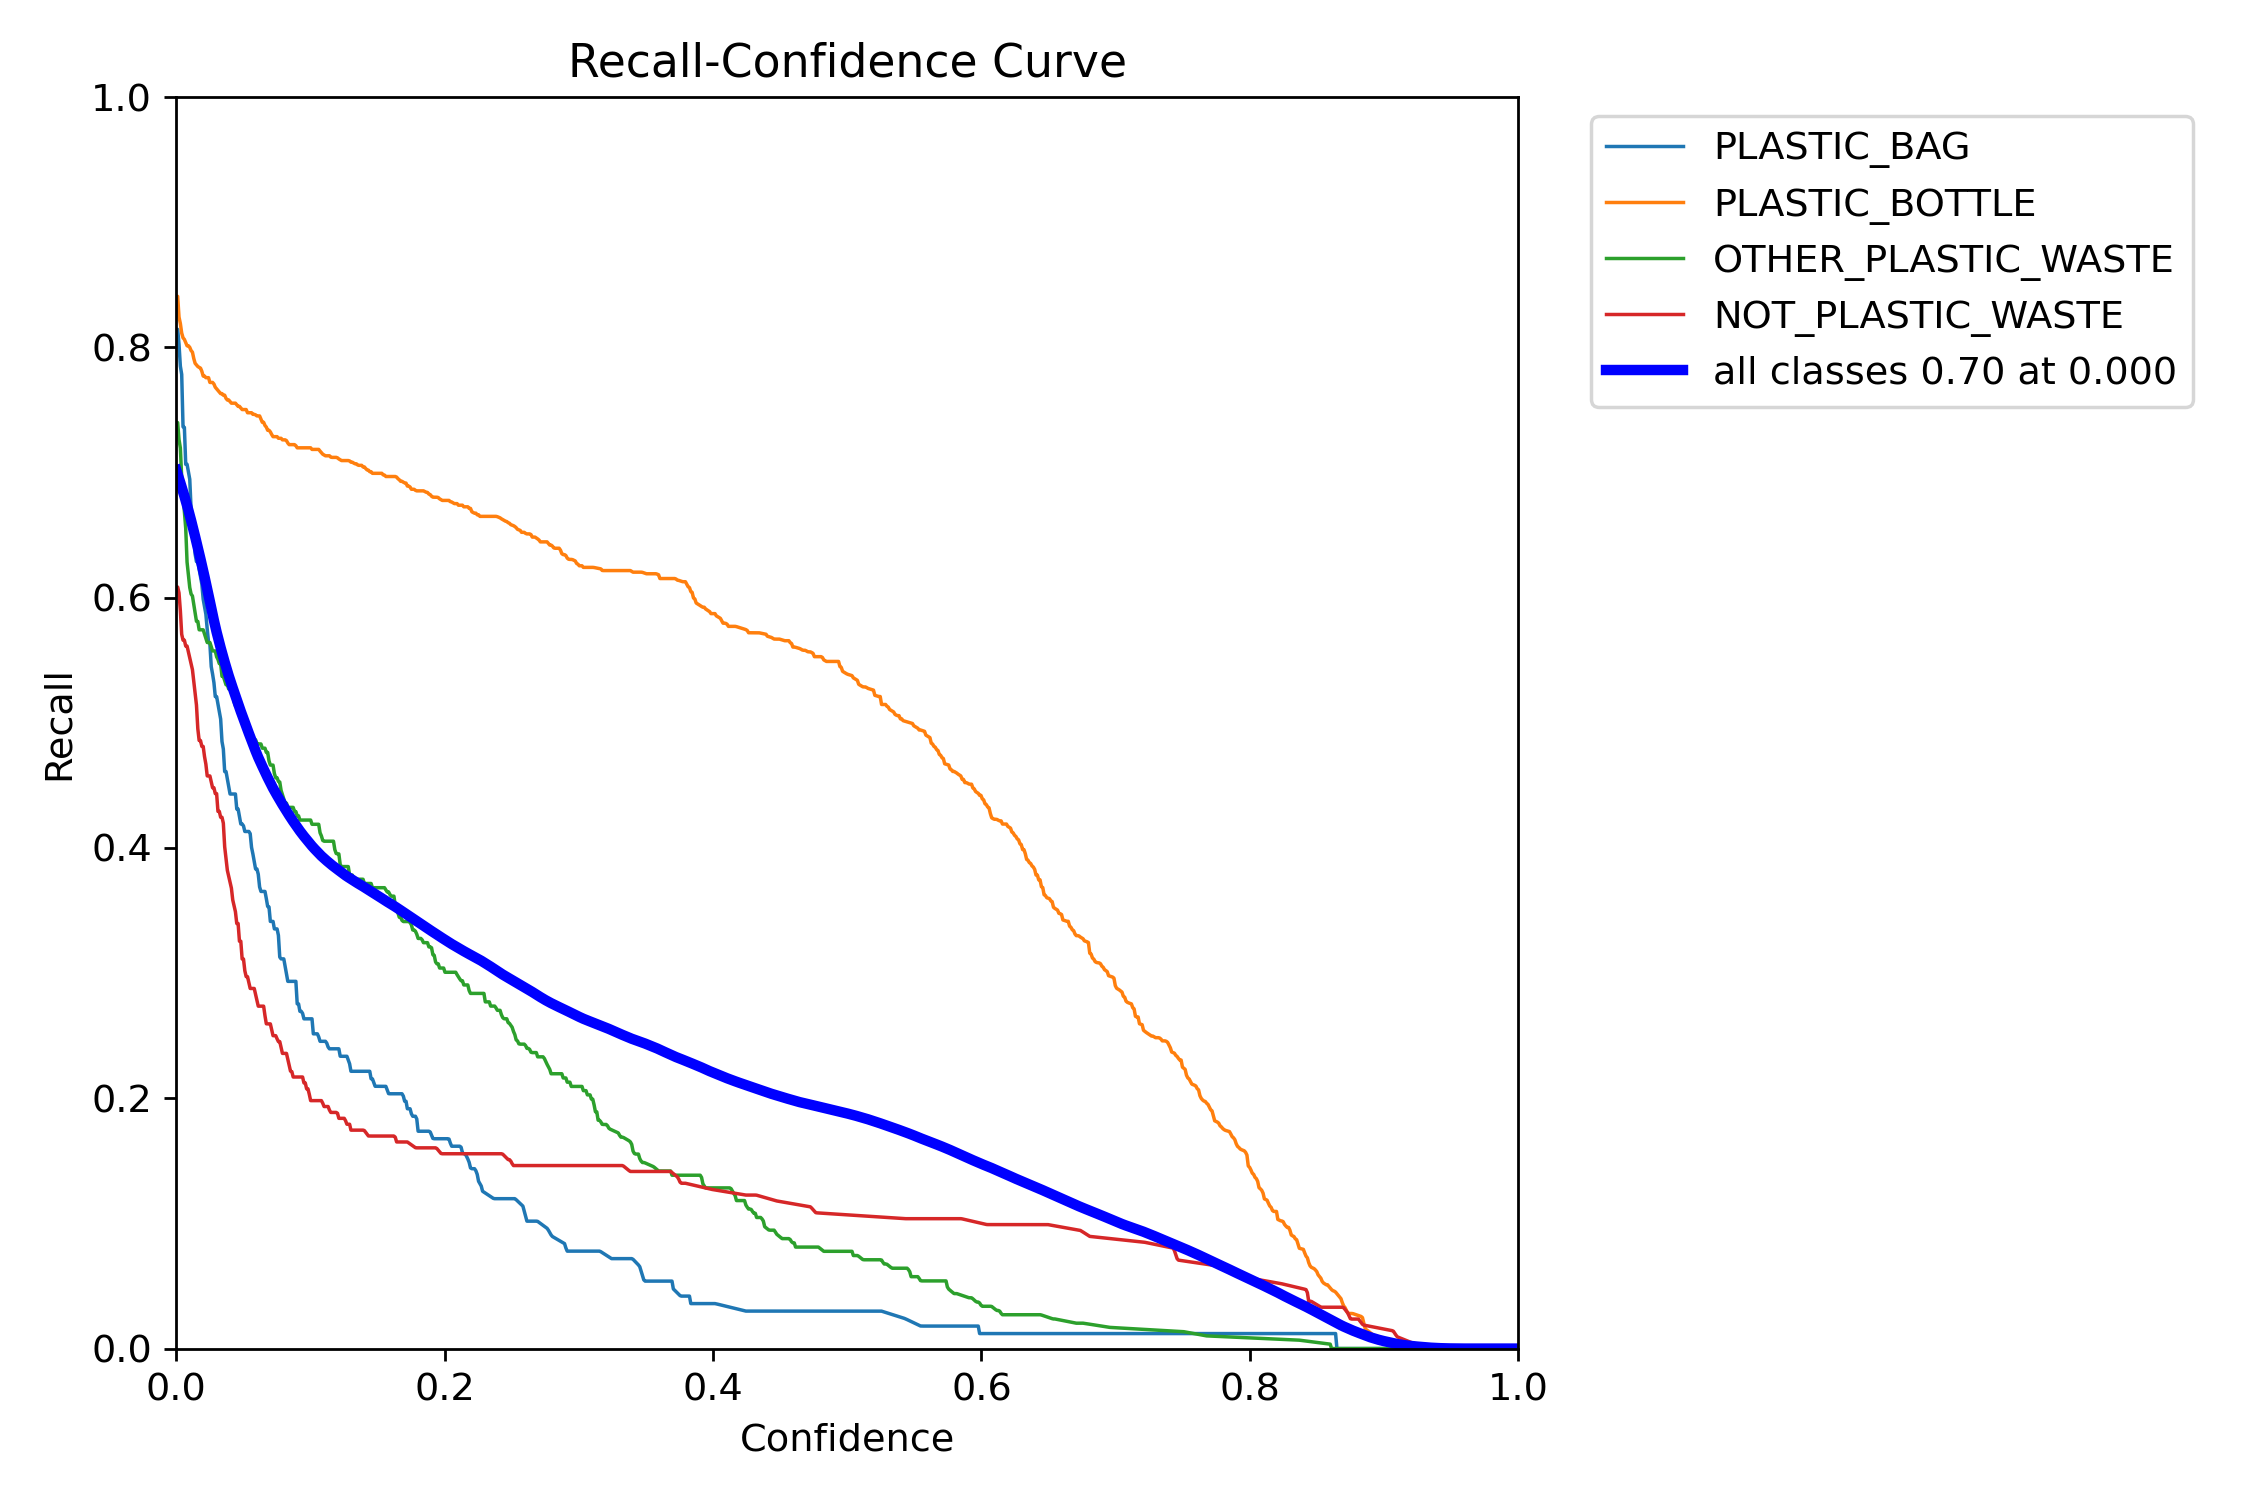
\includegraphics[width=.9\linewidth]{v_6/nano-tune-2.0/R_curve.png}
        \subcaption{PR-curve}
        \label{fig:v6-4.2}
    \end{subfigure}
    \vskip\baselineskip
    \begin{subfigure}{.5\textwidth}
        \centering
        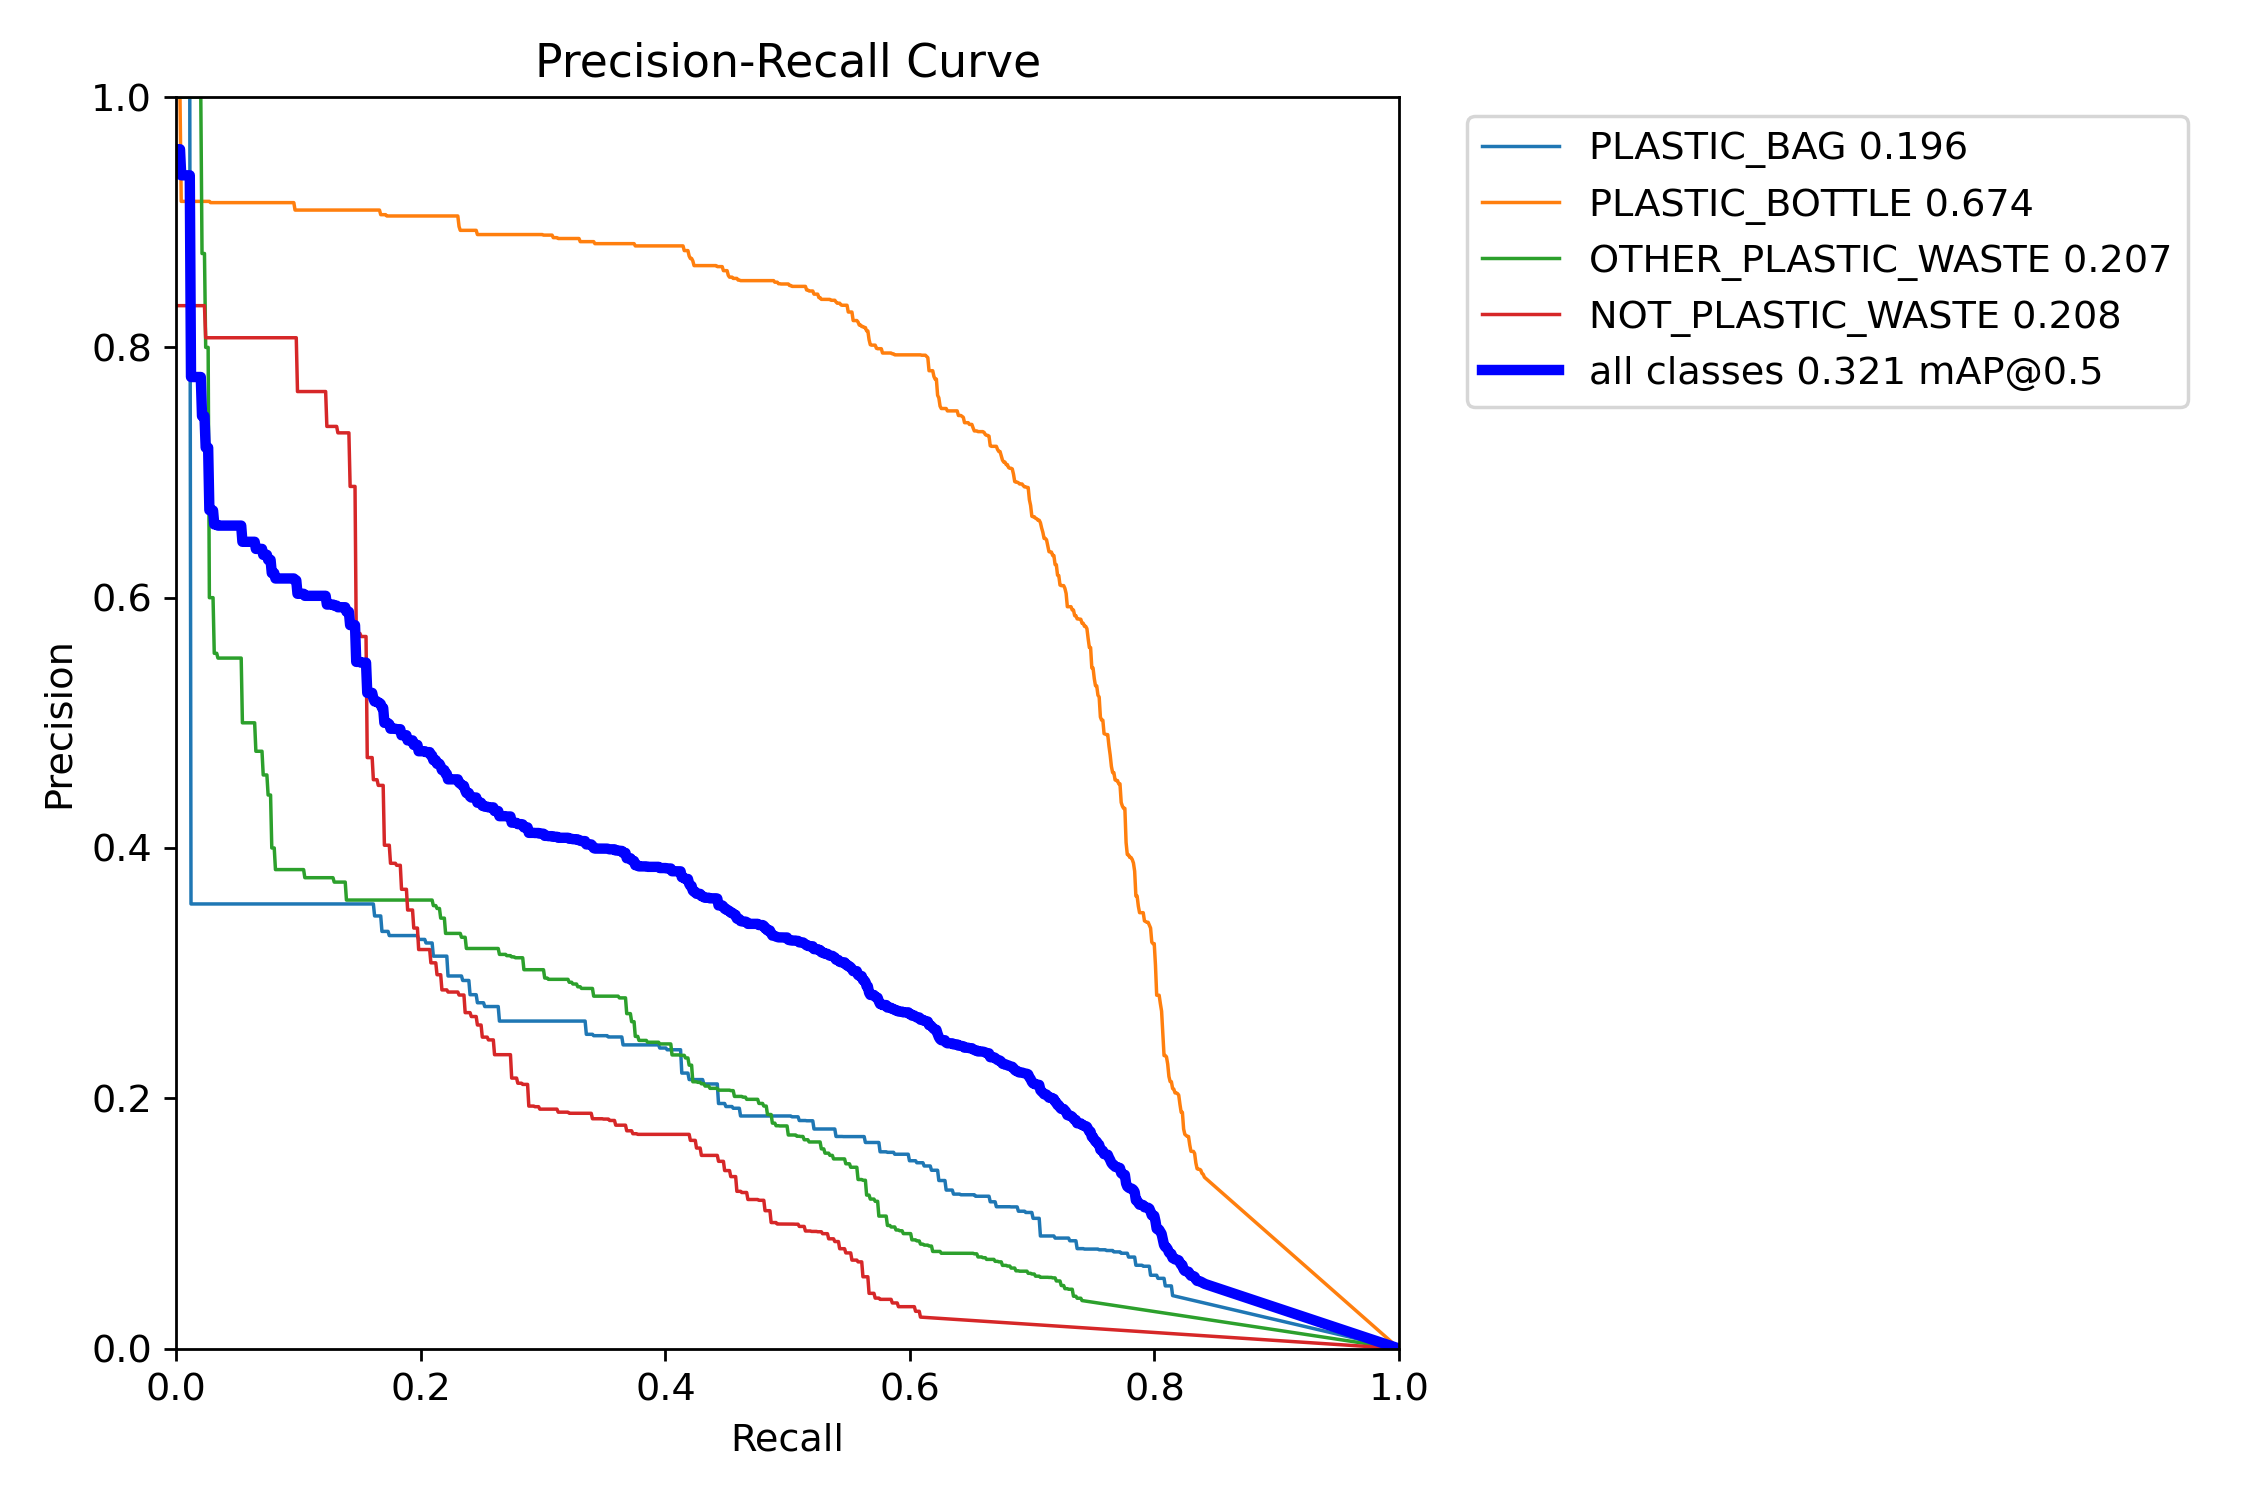
\includegraphics[width=.9\linewidth]{v_6/nano-tune-2.0/PR_curve.png}
        \subcaption{PR-curve}
        \label{fig:v6-4.3}
    \end{subfigure}
    \begin{subfigure}{.49\textwidth}
        \centering
        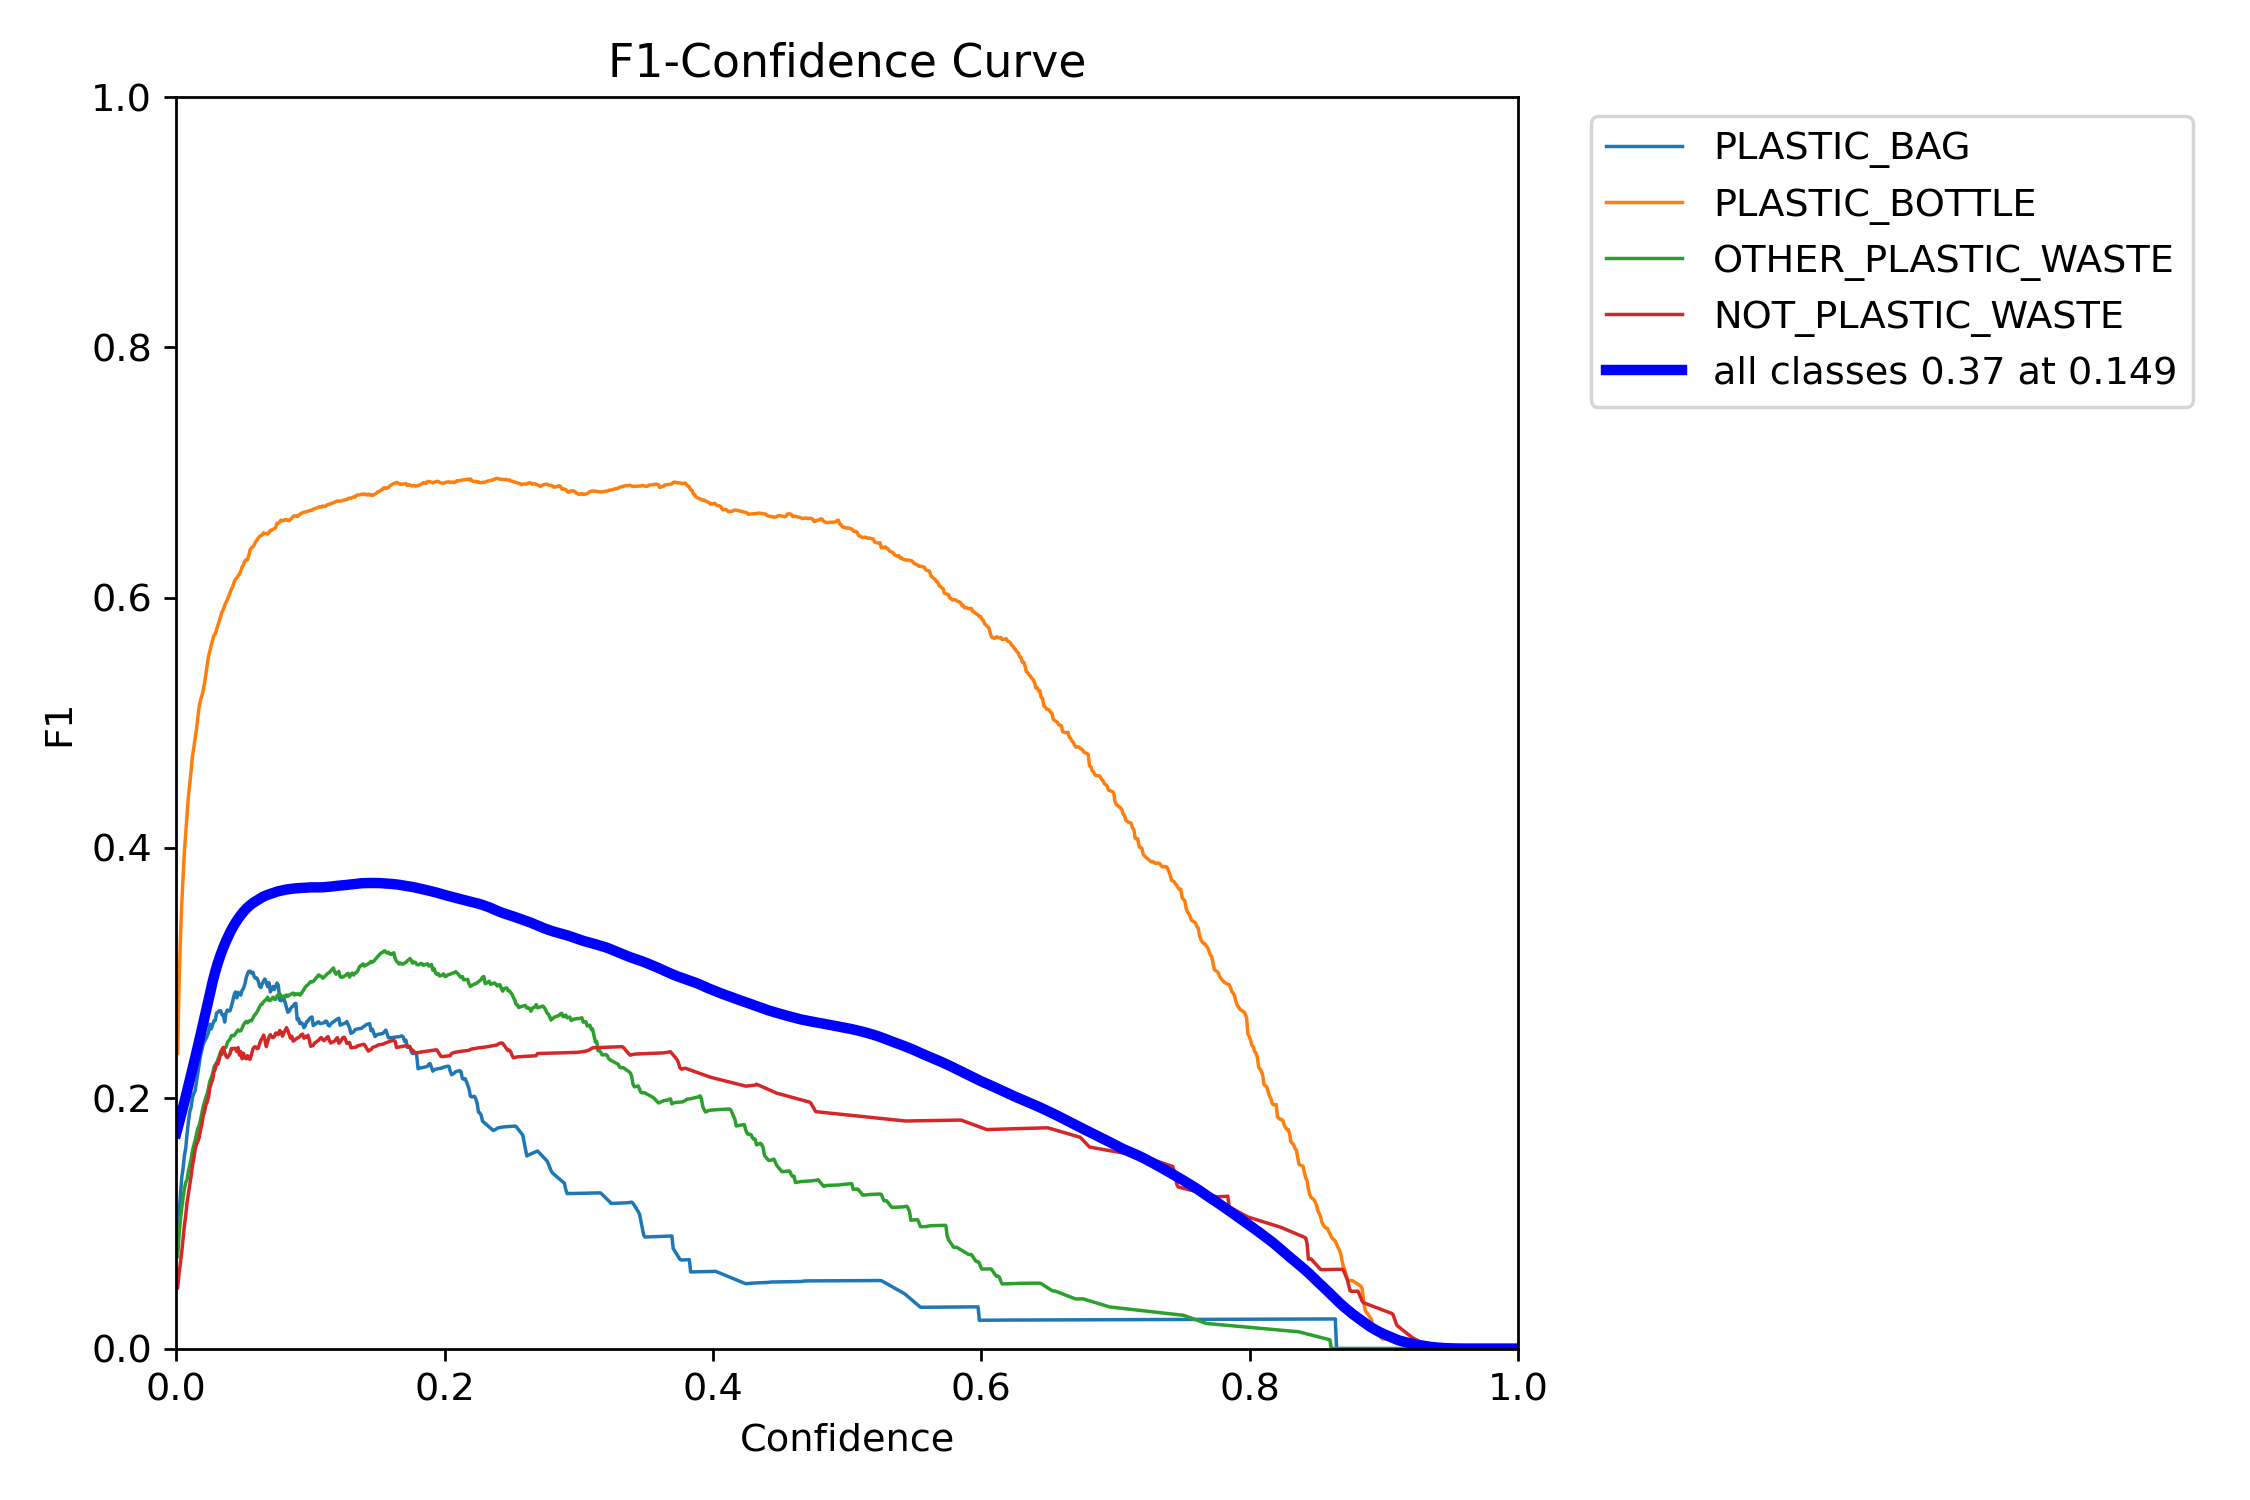
\includegraphics[width=.9\linewidth]{v_6/nano-tune-2.0/F1_curve.png}
        \subcaption{F1-curve}
        \label{fig:v6-4.4}
    \end{subfigure}
    
    \caption{Andamento funzioni di loss e metriche durante l'esecuzione di \texttt{nano-tune-2.0}}
    \label{fig:v6-4}
\end{figure}

\begin{figure}[!htb]
    \centering
    \begin{subfigure}{.5\textwidth}
        \centering
        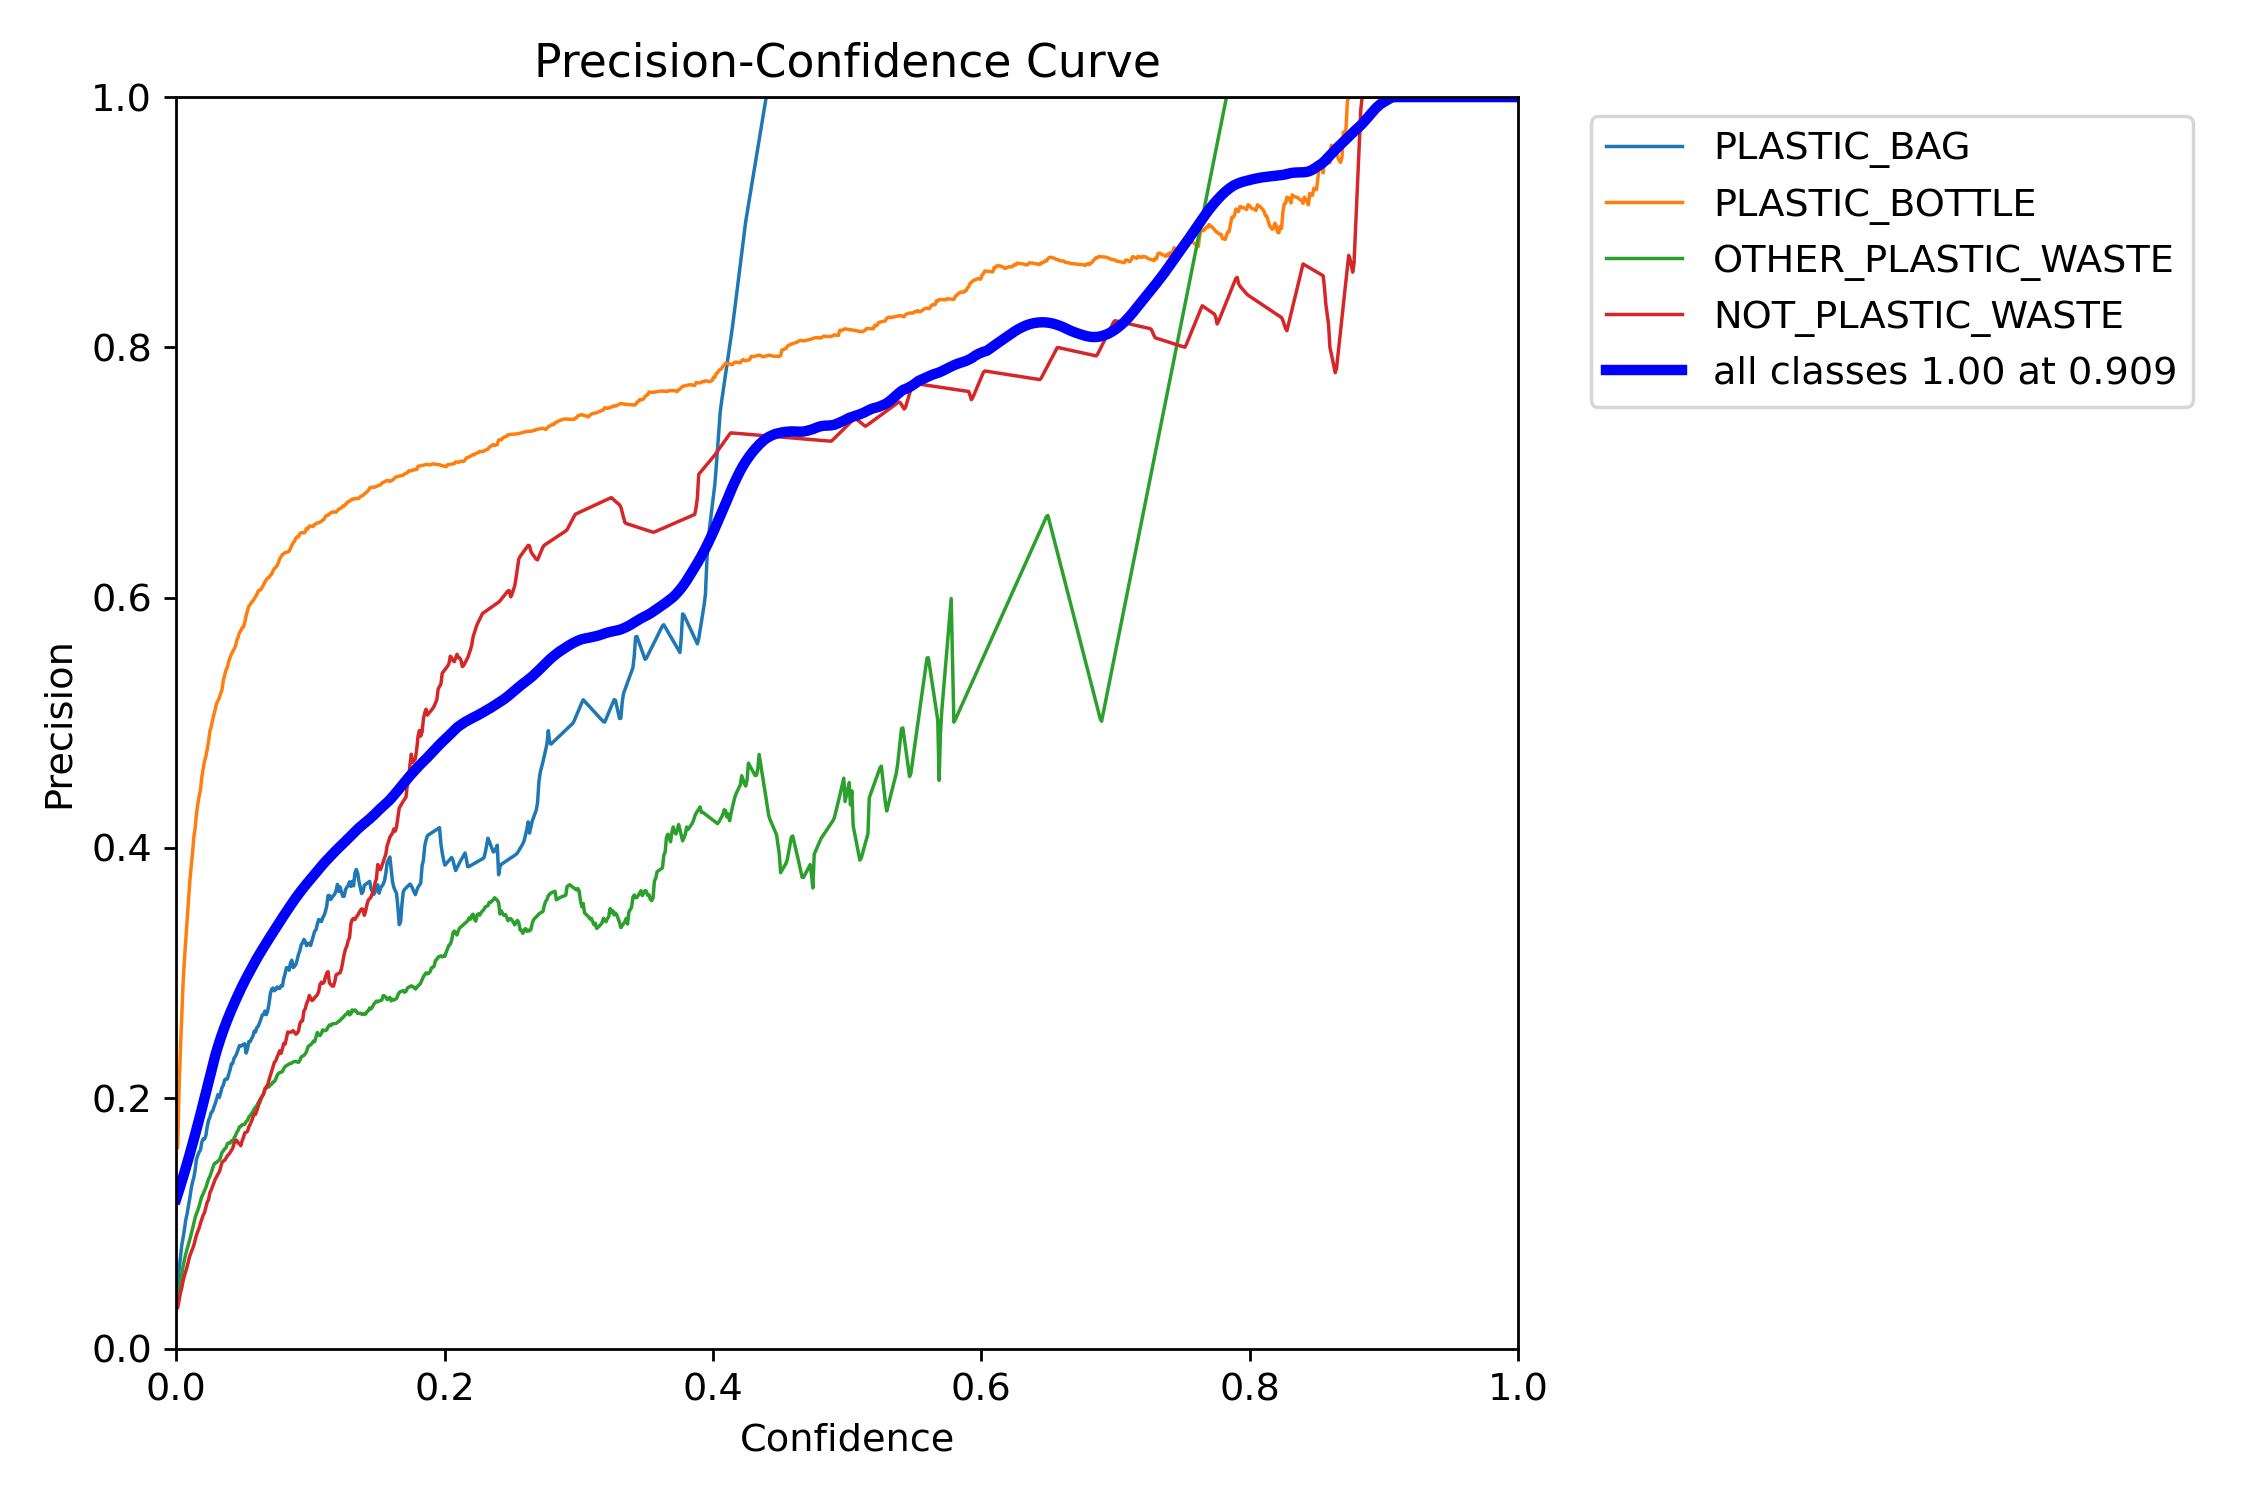
\includegraphics[width=.9\linewidth]{v_6/small-tune-2.0/P_curve.png}
        \subcaption{P-curve}
        \label{fig:v6-5.1}
    \end{subfigure}%
      \begin{subfigure}{.5\textwidth}
        \centering
        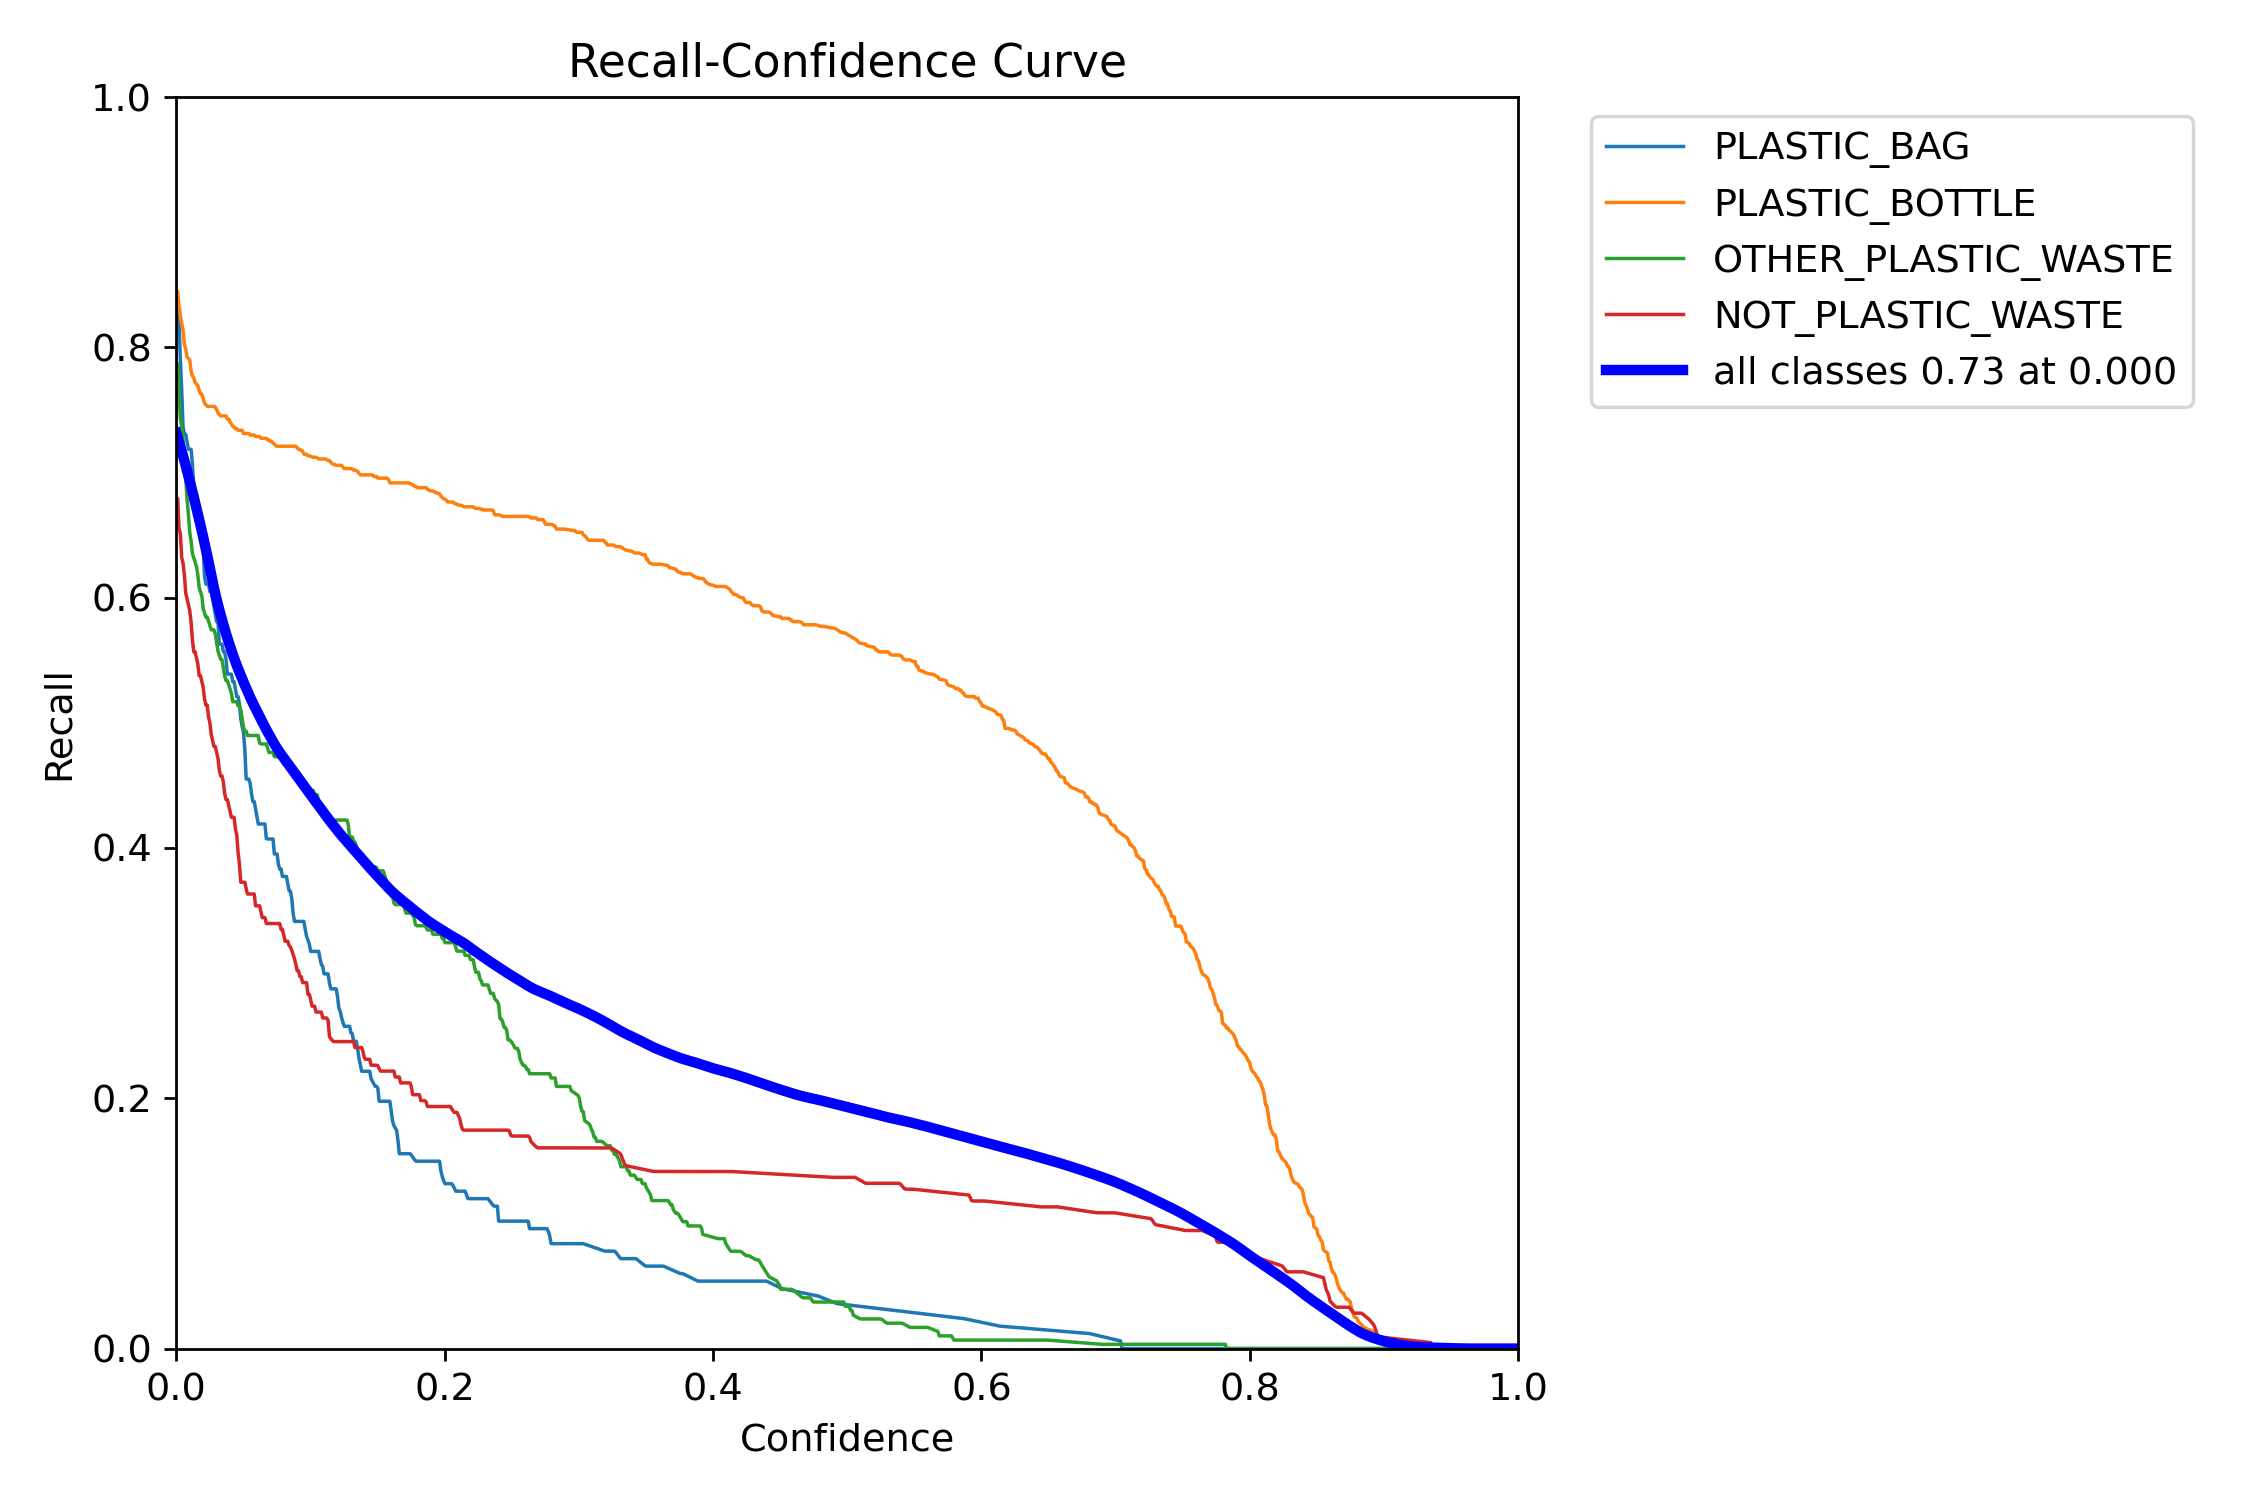
\includegraphics[width=.9\linewidth]{v_6/small-tune-2.0/R_curve.png}
        \subcaption{PR-curve}
        \label{fig:v6-5.2}
    \end{subfigure}
    \vskip\baselineskip
    \begin{subfigure}{.5\textwidth}
        \centering
        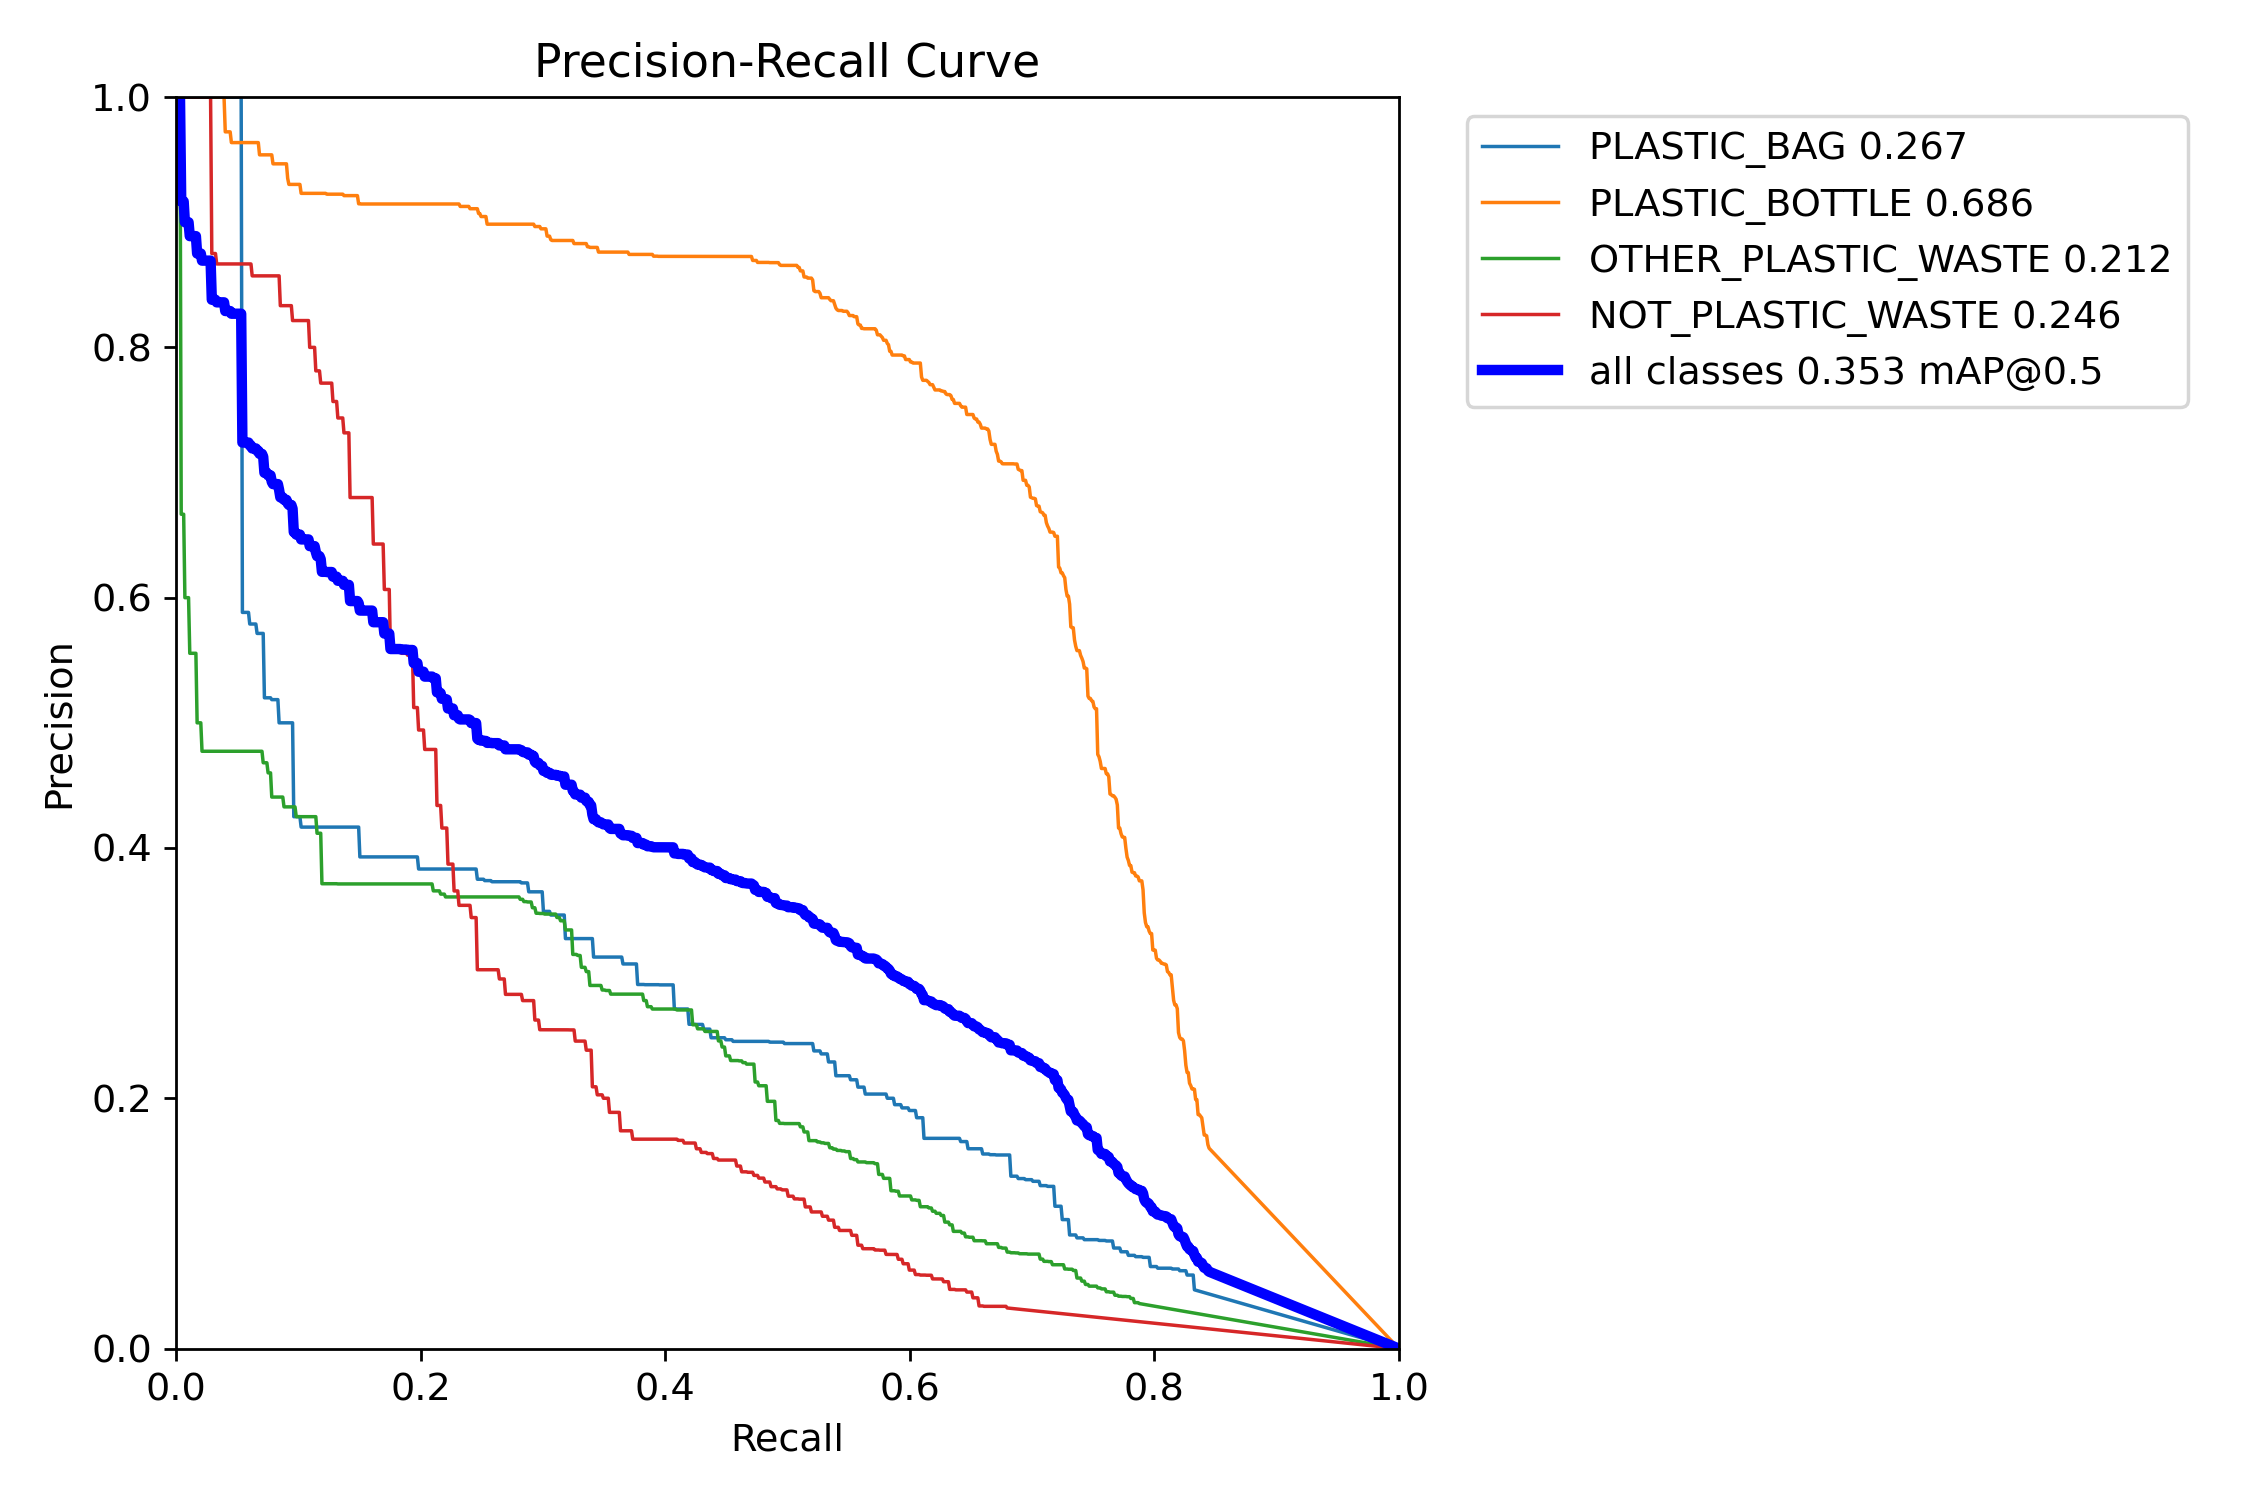
\includegraphics[width=.9\linewidth]{v_6/small-tune-2.0/PR_curve.png}
        \subcaption{PR-curve}
        \label{fig:v6-5.3}
    \end{subfigure}
    \begin{subfigure}{.49\textwidth}
        \centering
        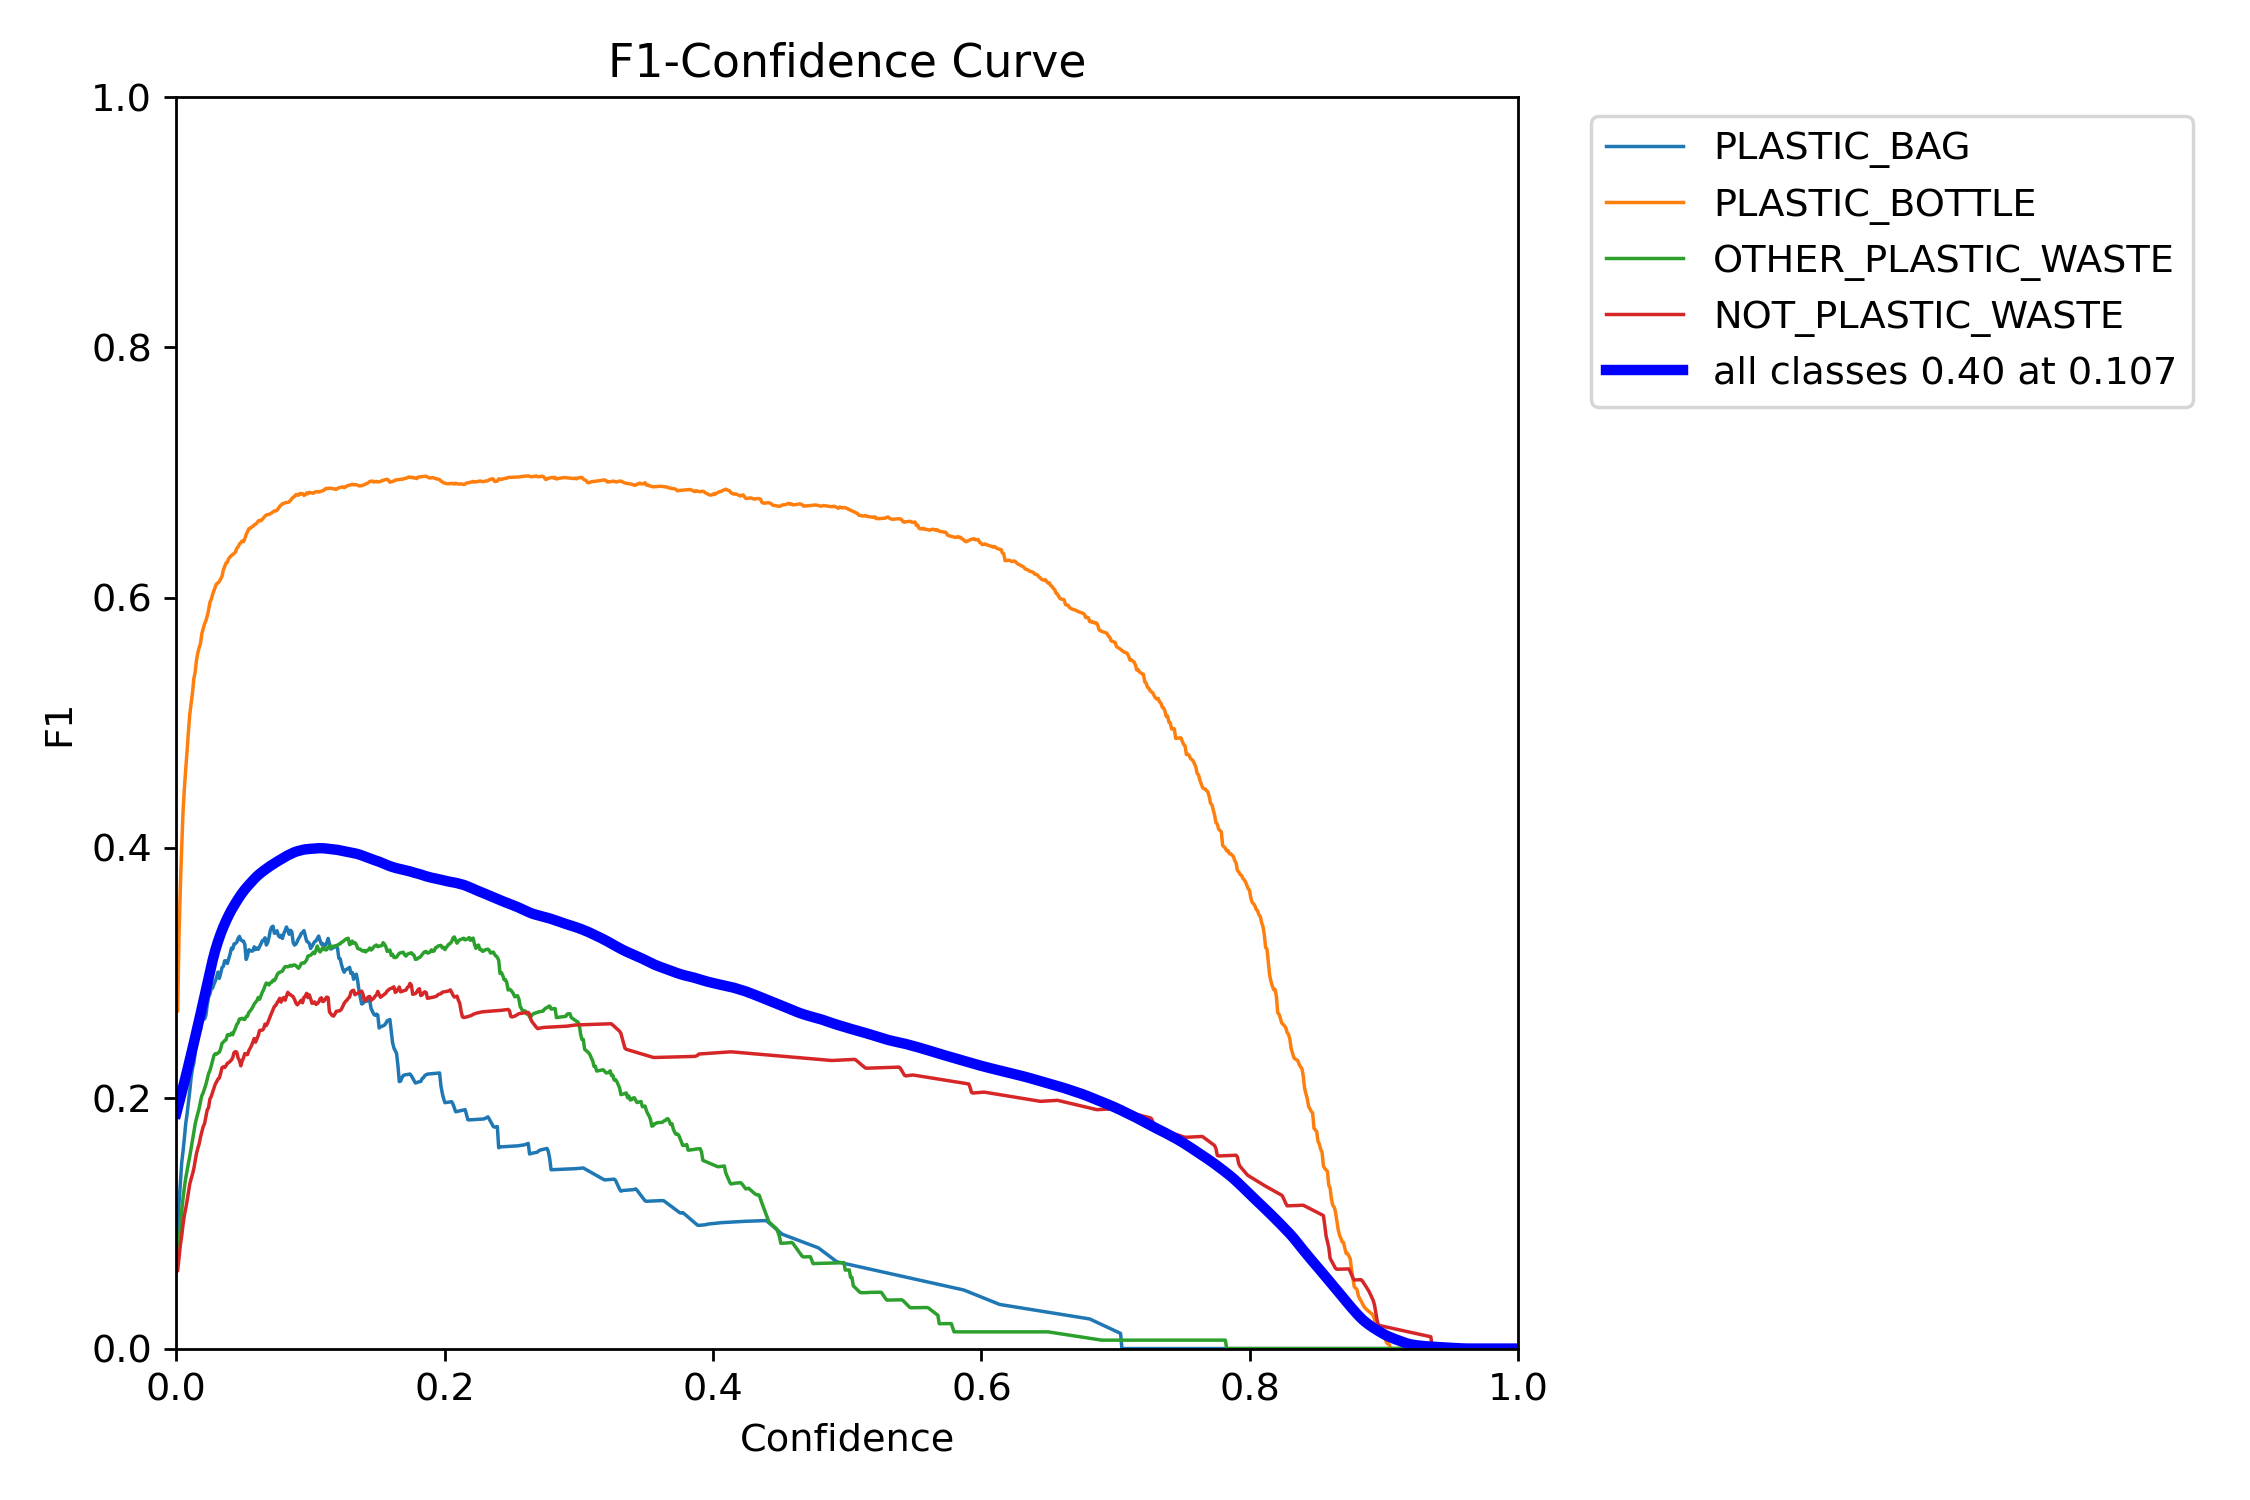
\includegraphics[width=.9\linewidth]{v_6/small-tune-2.0/F1_curve.png}
        \subcaption{F1-curve}
        \label{fig:v6-5.4}
    \end{subfigure}
    
    \caption{Andamento funzioni di loss e metriche durante l'esecuzione di \texttt{small-tune-2.0}}
    \label{fig:v6-5}
\end{figure}

\begin{figure}[!htb]
    \centering
    \begin{subfigure}{.5\textwidth}
        \centering
        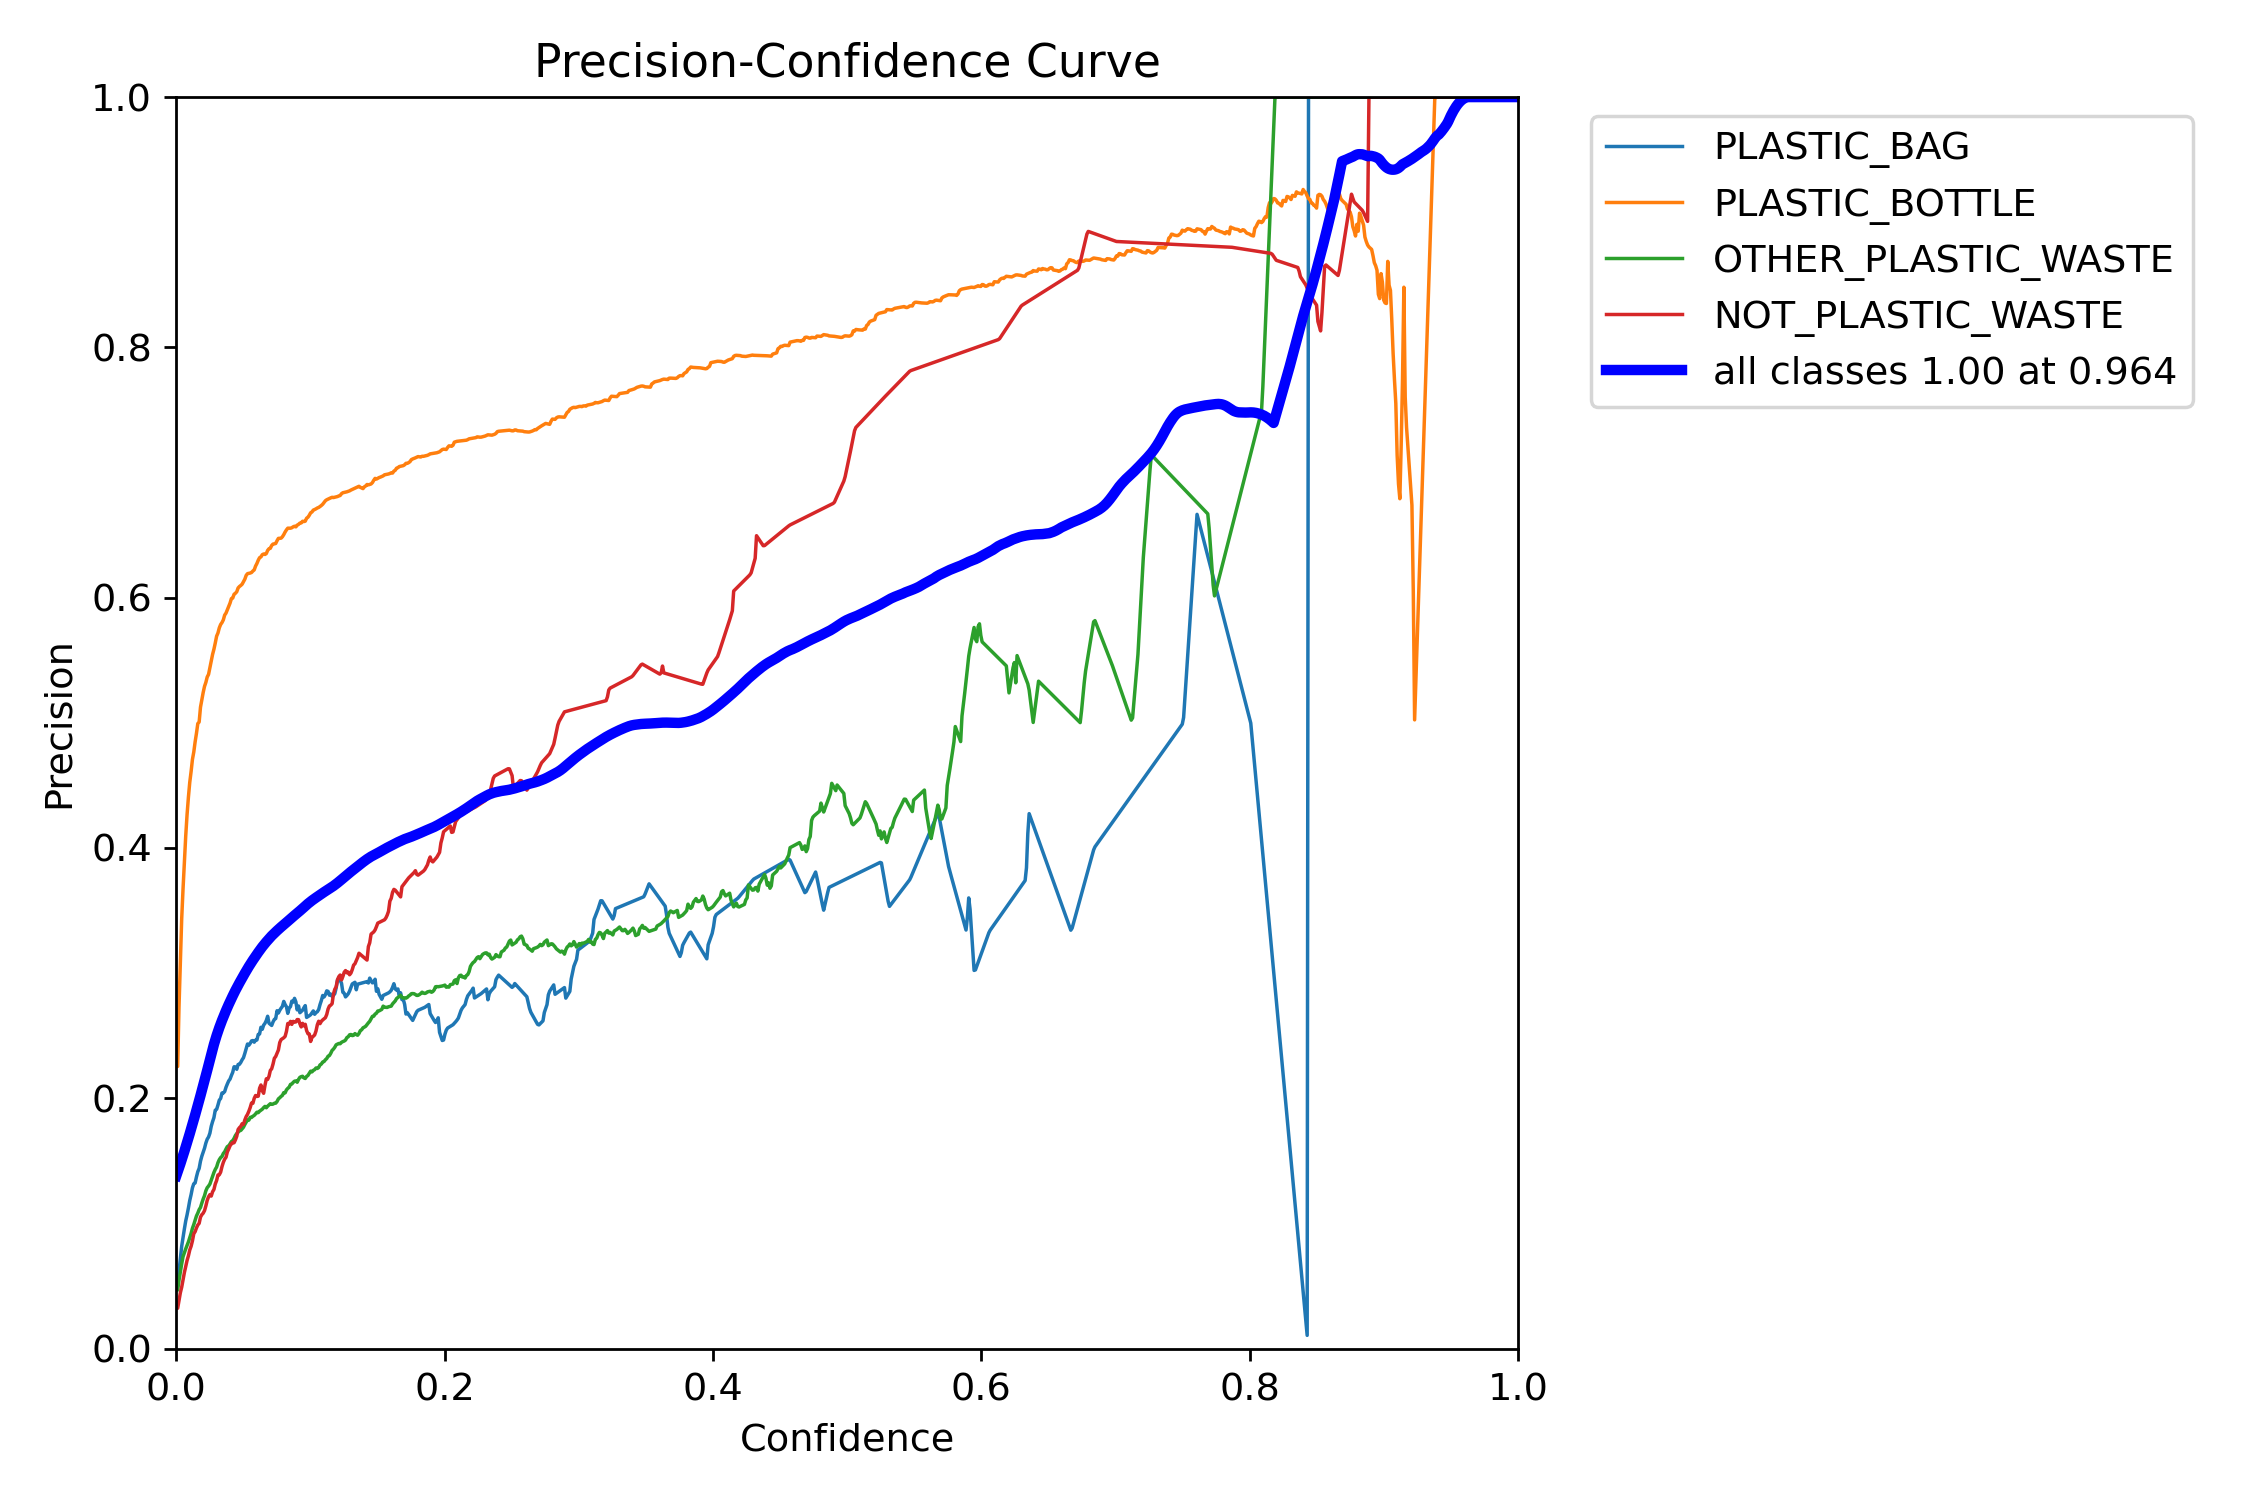
\includegraphics[width=.9\linewidth]{v_6/medium-tune-2.0/P_curve.png}
        \subcaption{P-curve}
        \label{fig:v6-6.1}
    \end{subfigure}%
      \begin{subfigure}{.5\textwidth}
        \centering
        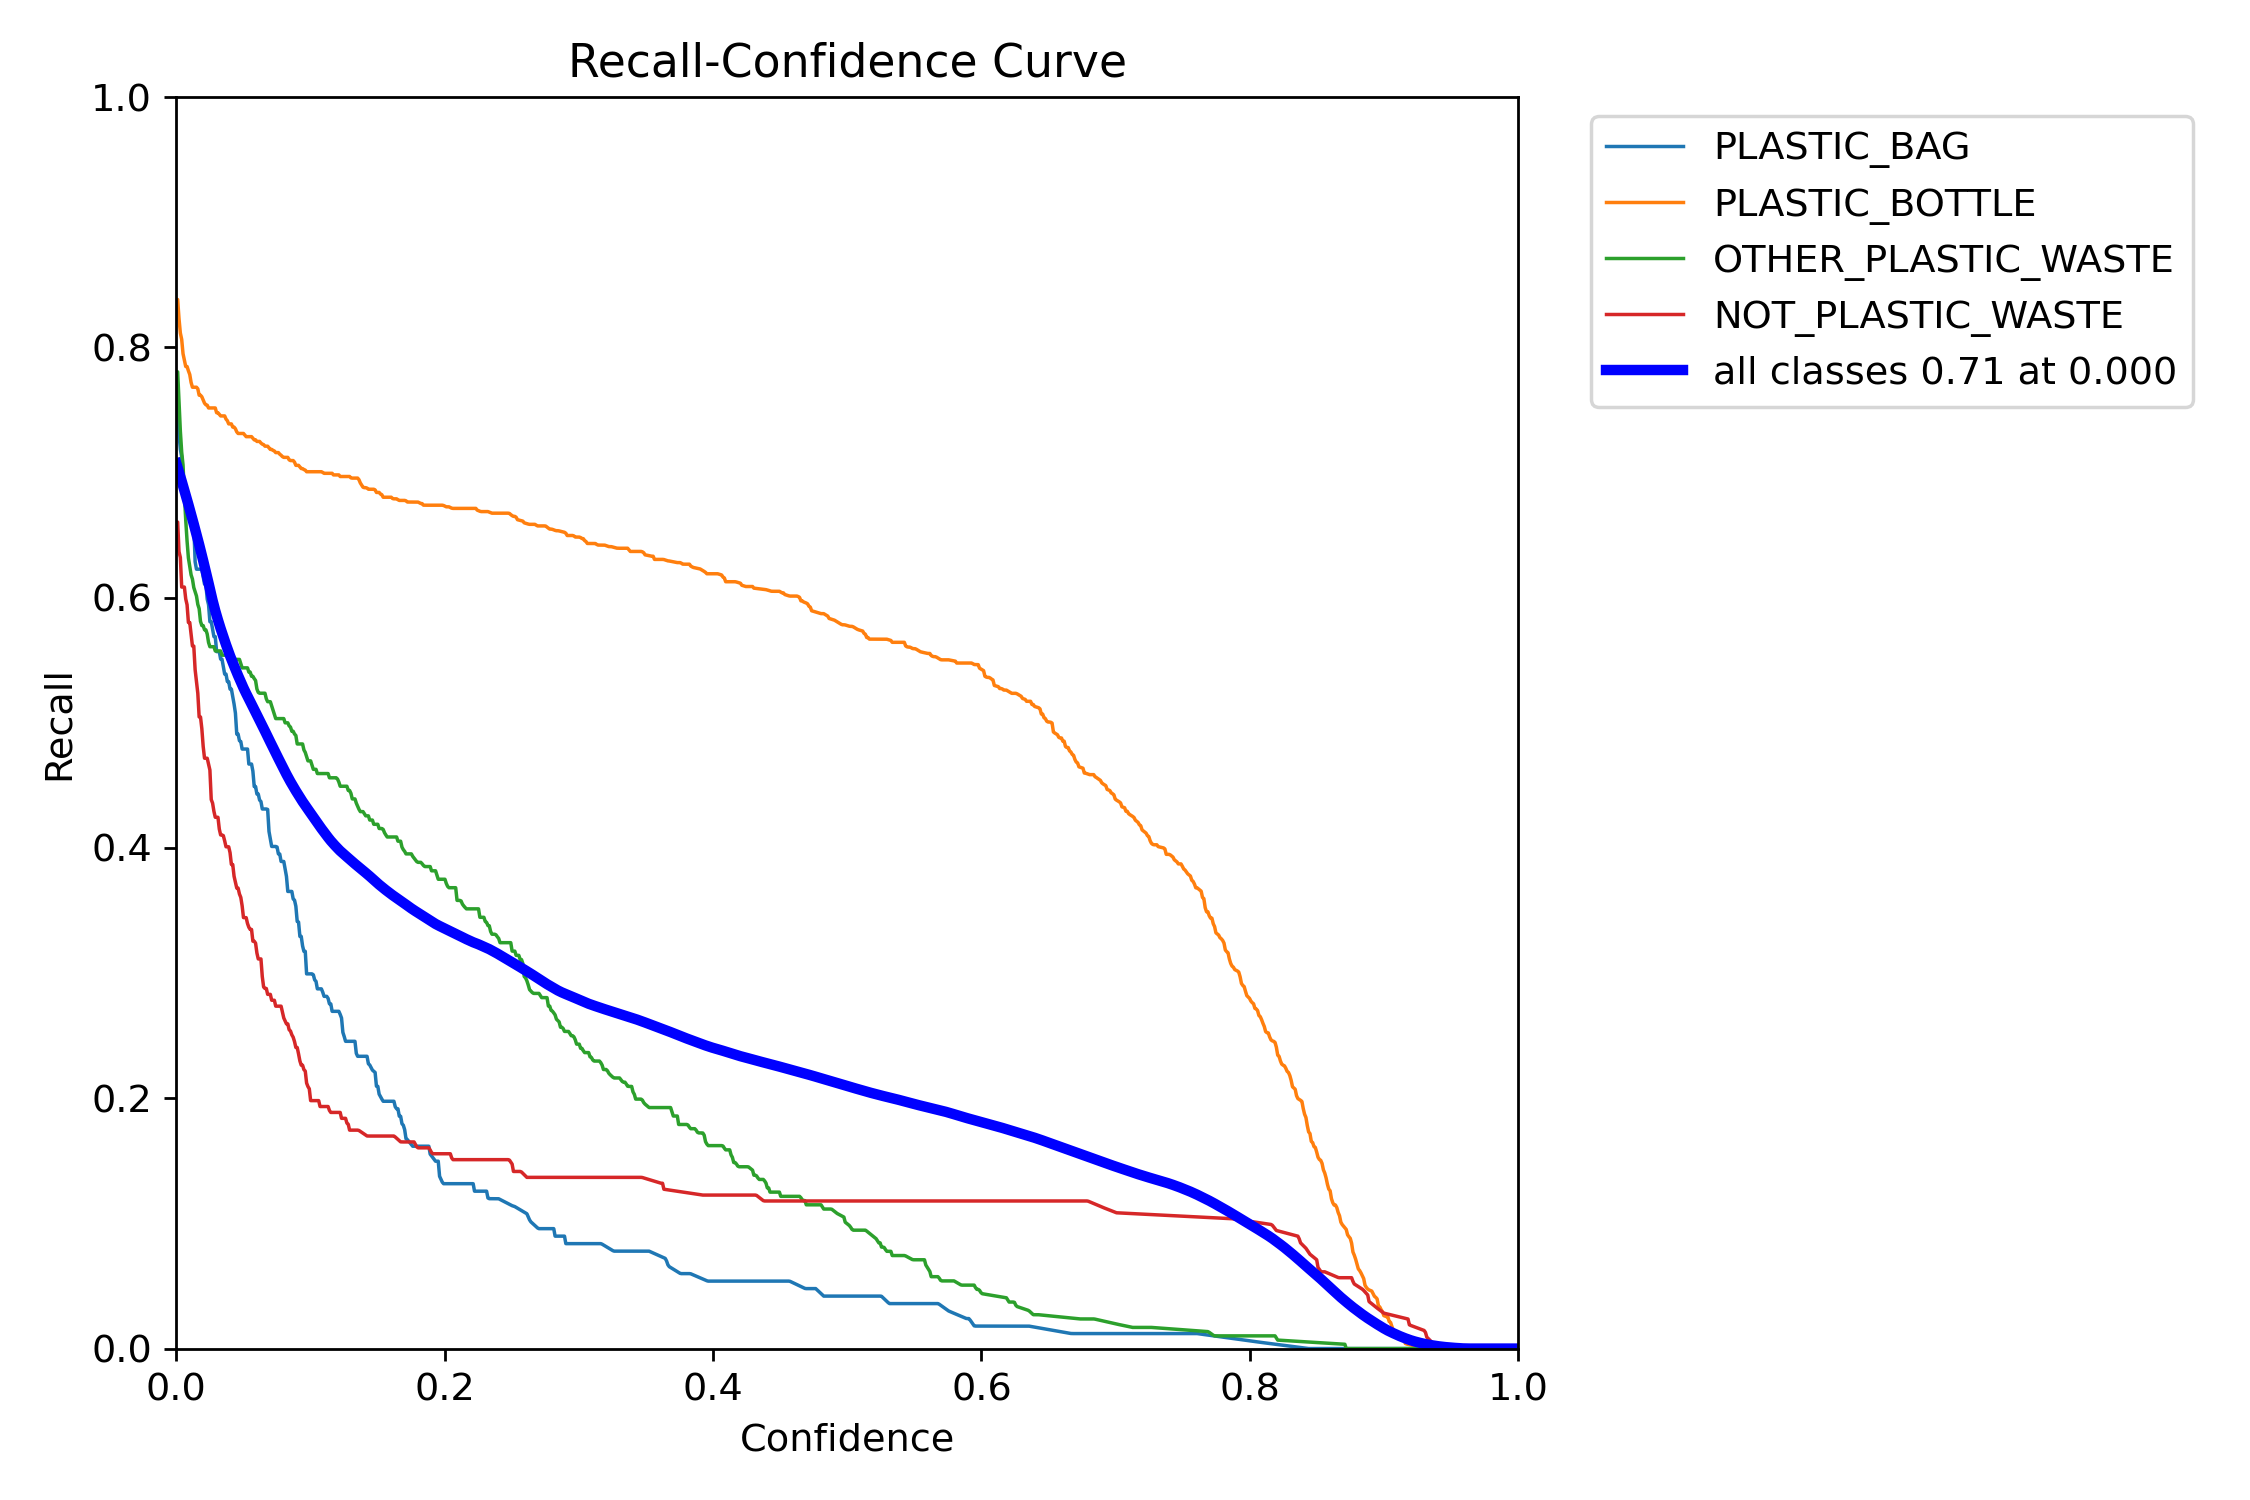
\includegraphics[width=.9\linewidth]{v_6/medium-tune-2.0/R_curve.png}
        \subcaption{PR-curve}
        \label{fig:v6-6.2}
    \end{subfigure}
    \vskip\baselineskip
    \begin{subfigure}{.5\textwidth}
        \centering
        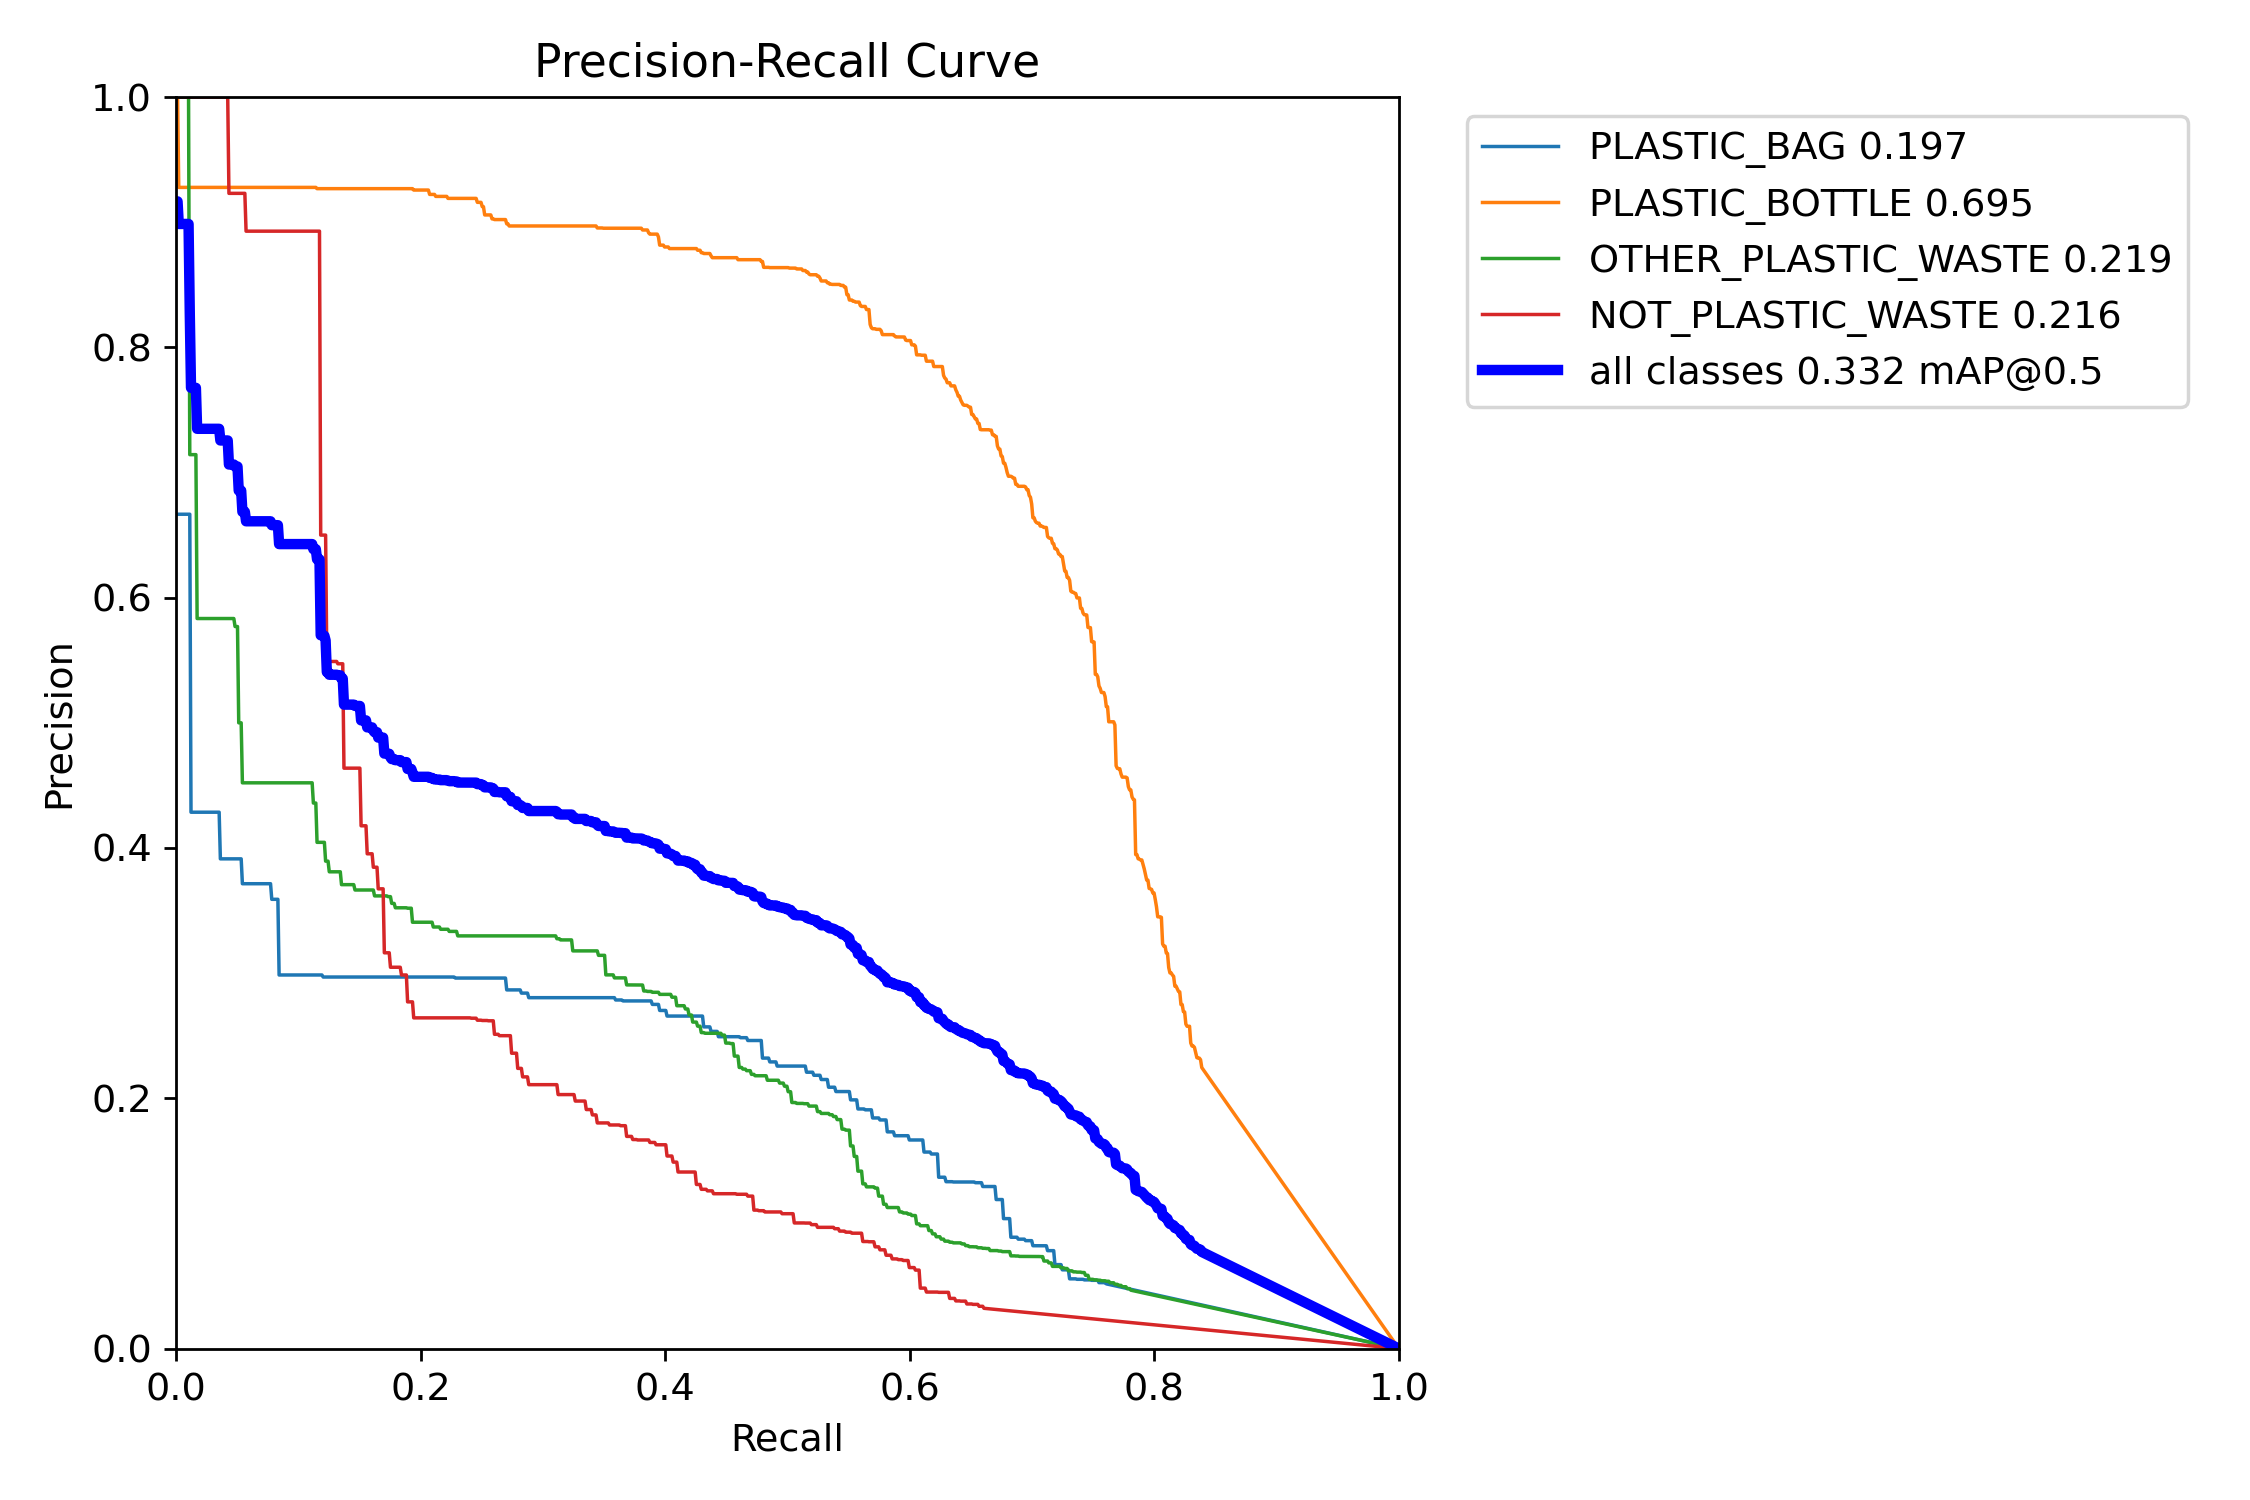
\includegraphics[width=.9\linewidth]{v_6/medium-tune-2.0/PR_curve.png}
        \subcaption{PR-curve}
        \label{fig:v6-6.3}
    \end{subfigure}
    \begin{subfigure}{.49\textwidth}
        \centering
        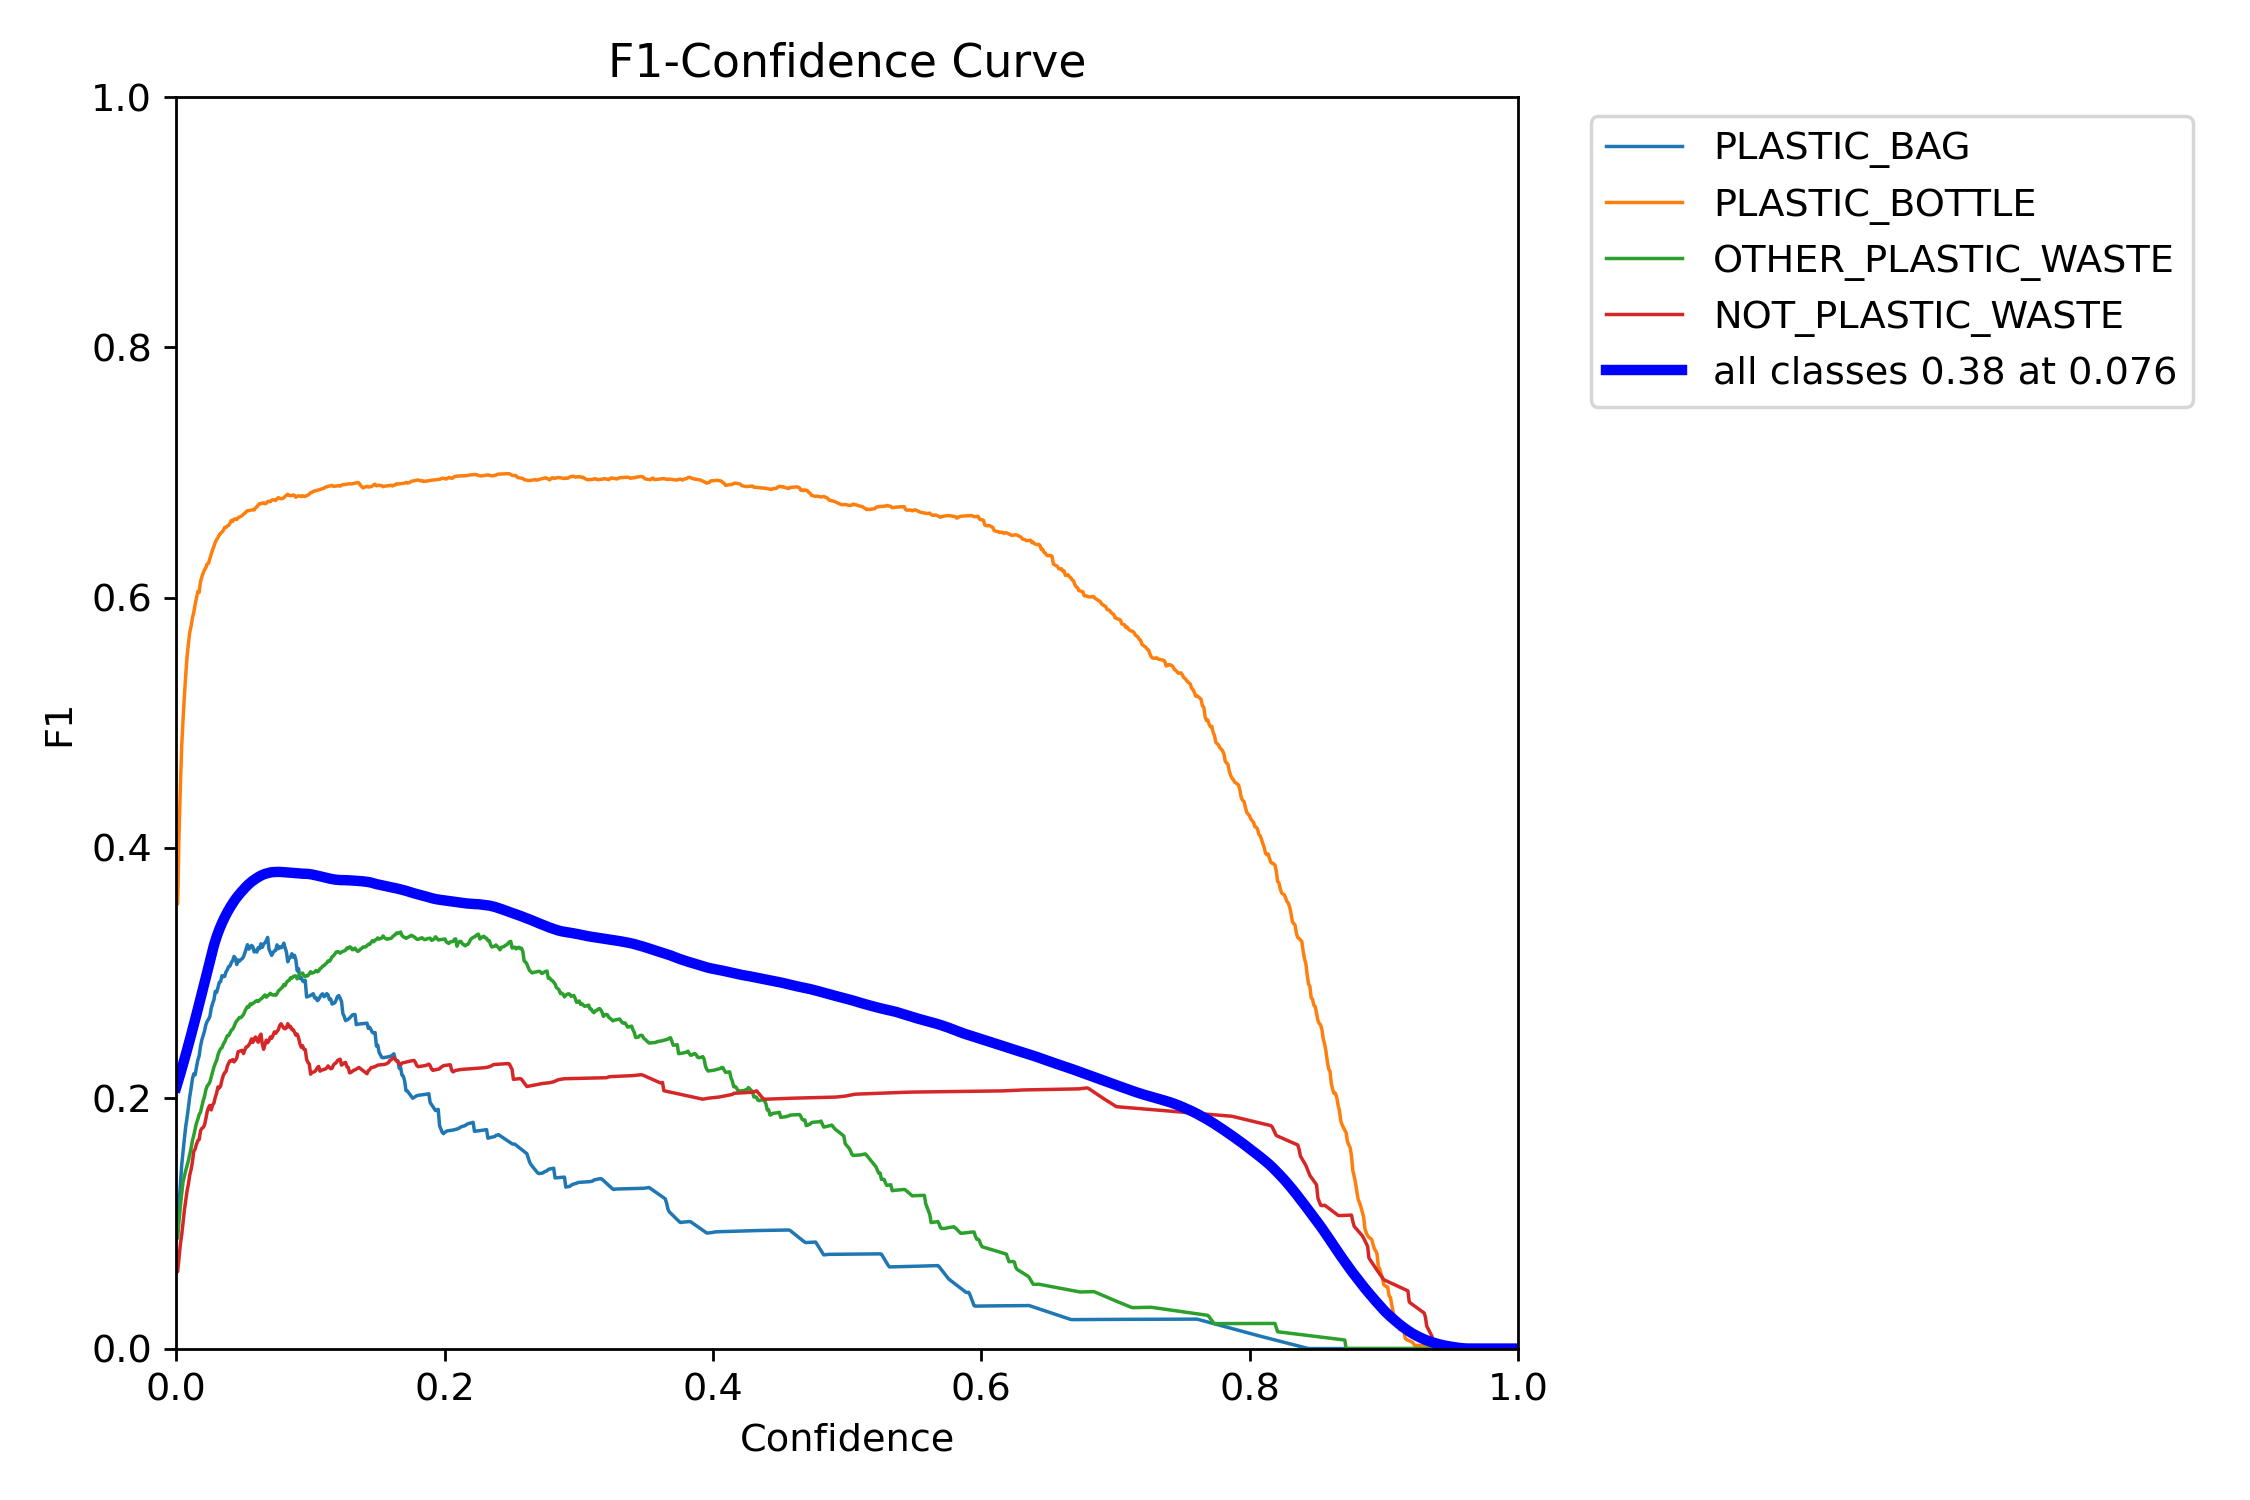
\includegraphics[width=.9\linewidth]{v_6/medium-tune-2.0/F1_curve.png}
        \subcaption{F1-curve}
        \label{fig:v6-6.4}
    \end{subfigure}
    
    \caption{Andamento funzioni di loss e metriche durante l'esecuzione di \texttt{medium-tune-2.0}}
    \label{fig:v6-6}
\end{figure}

\begin{figure}[!htb]
    \centering
    \begin{subfigure}{.49\textwidth}
        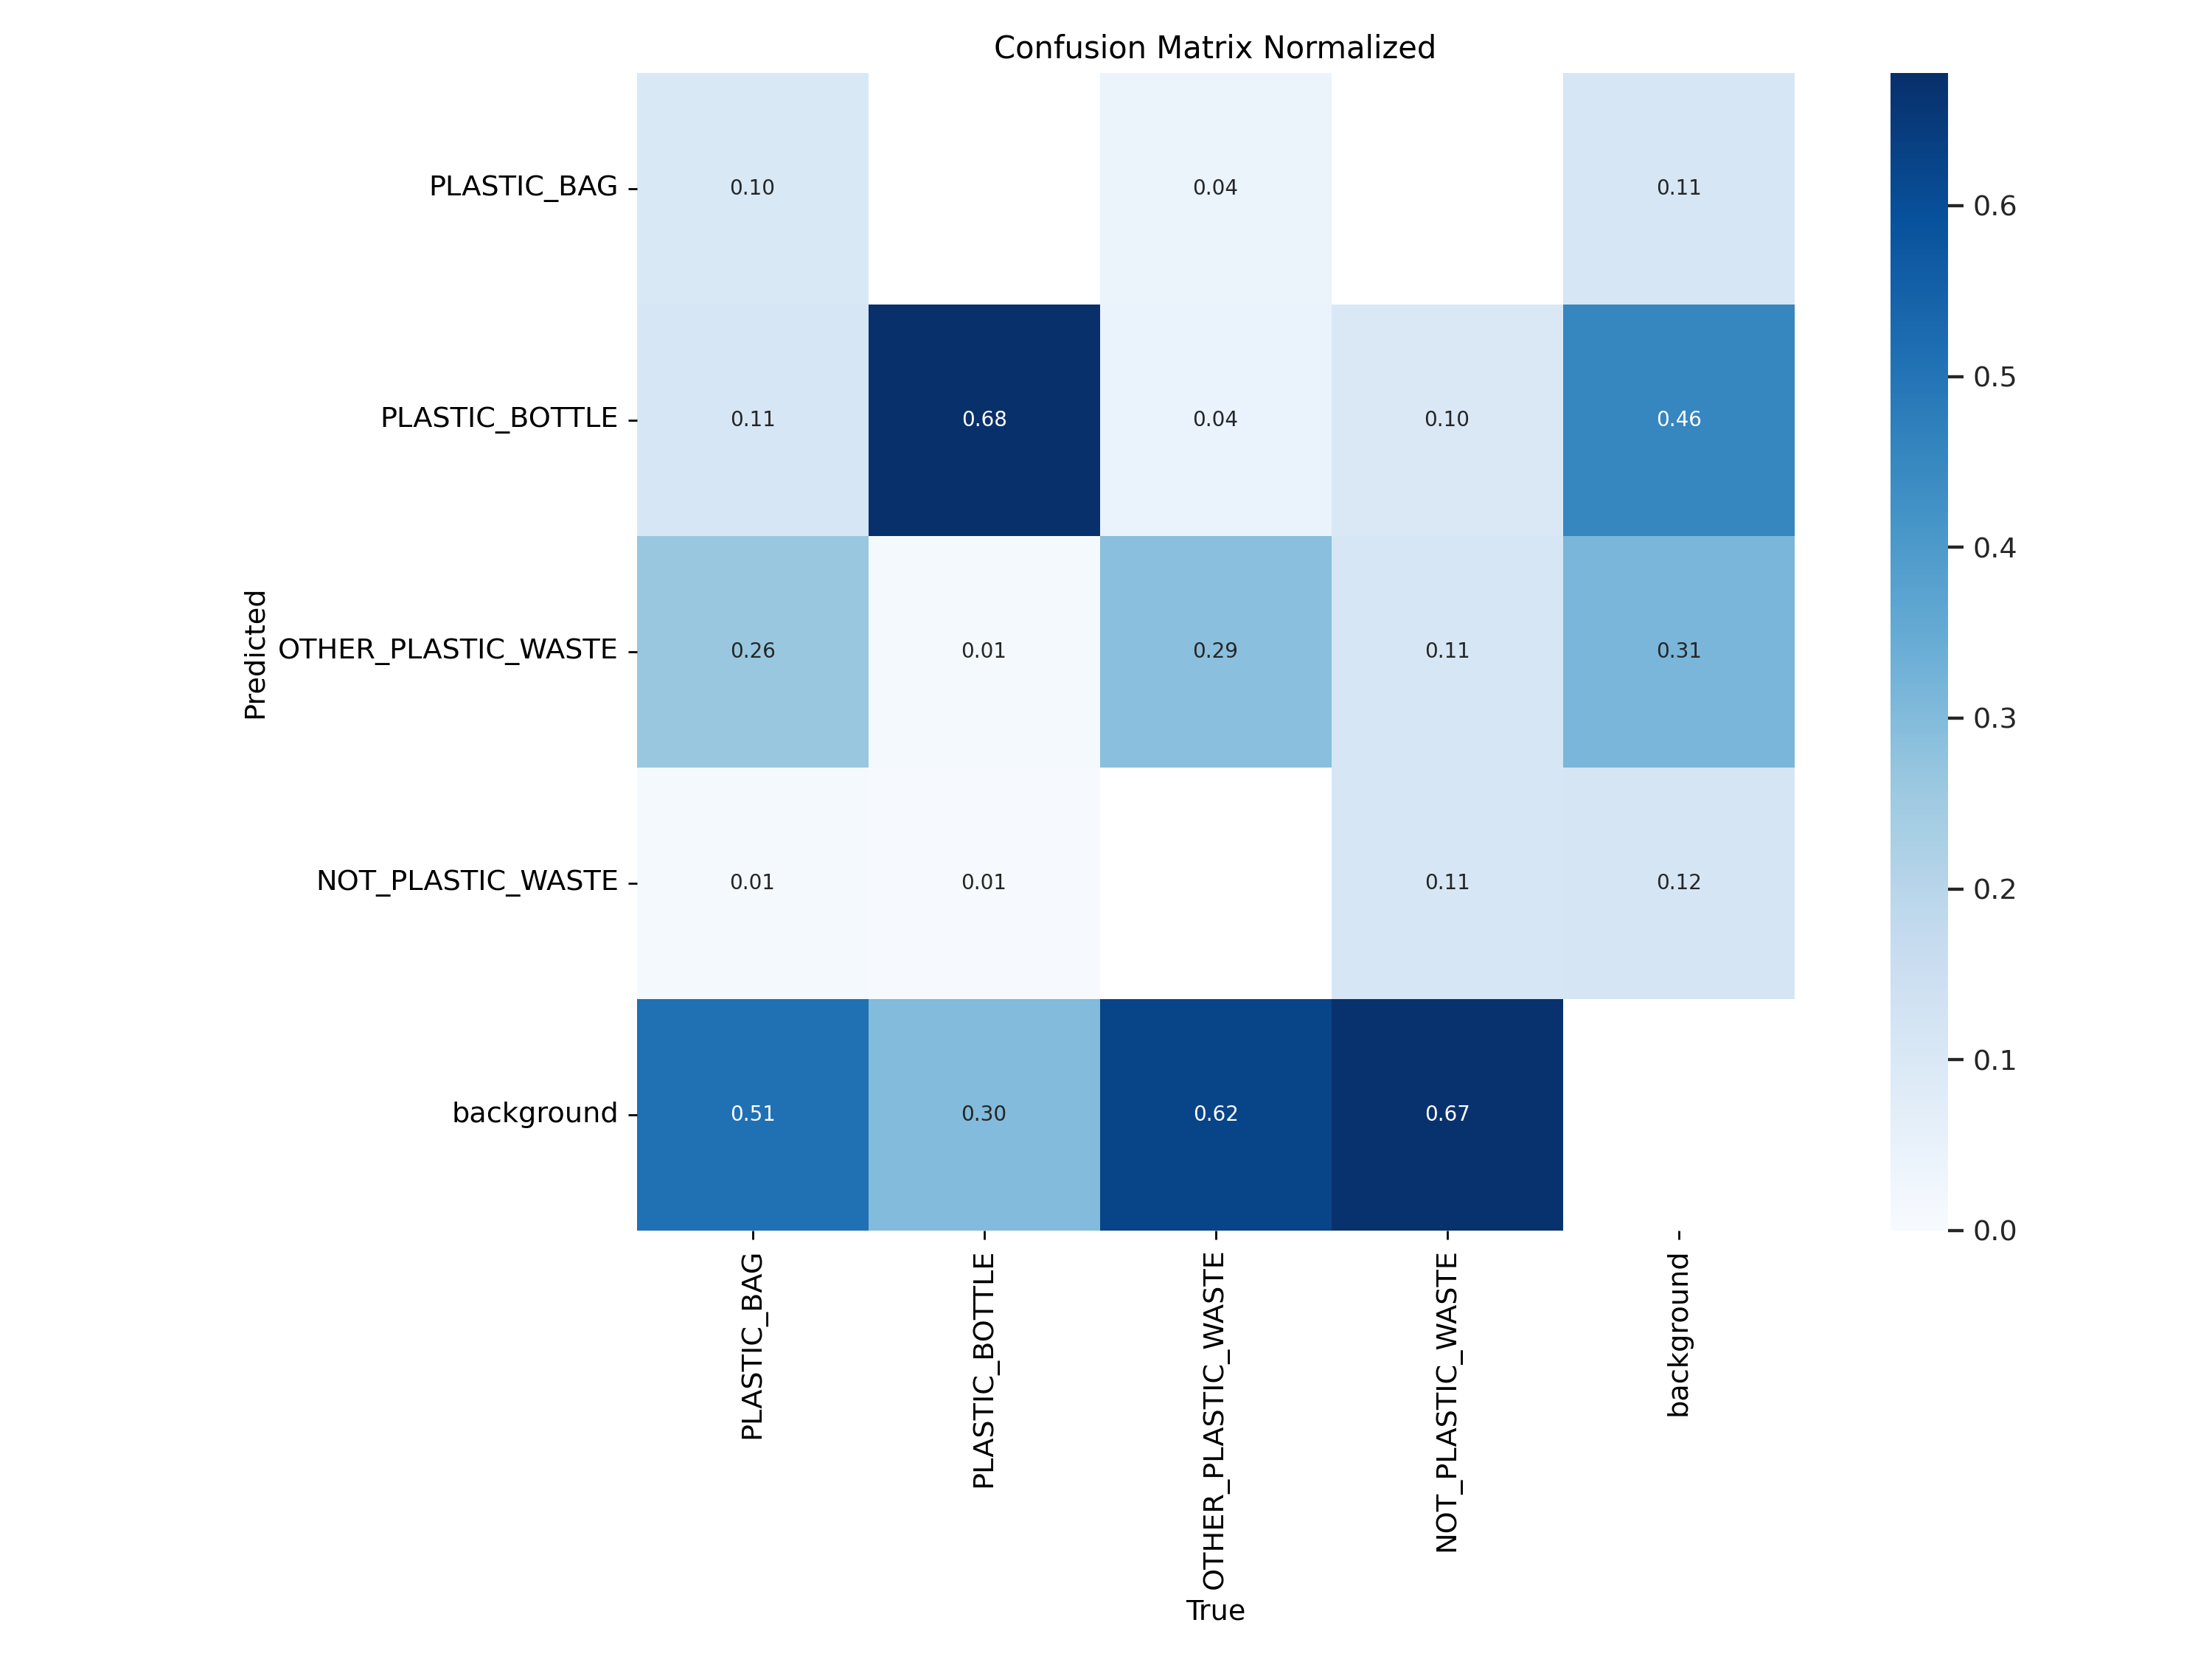
\includegraphics[width=0.9\textwidth]{v_6/nano-tune-2.0/confusion_matrix_normalized.png}
        \subcaption{Nano}
        \label{fig:v6-7.1}
    \end{subfigure}
    \begin{subfigure}{.49\textwidth}
        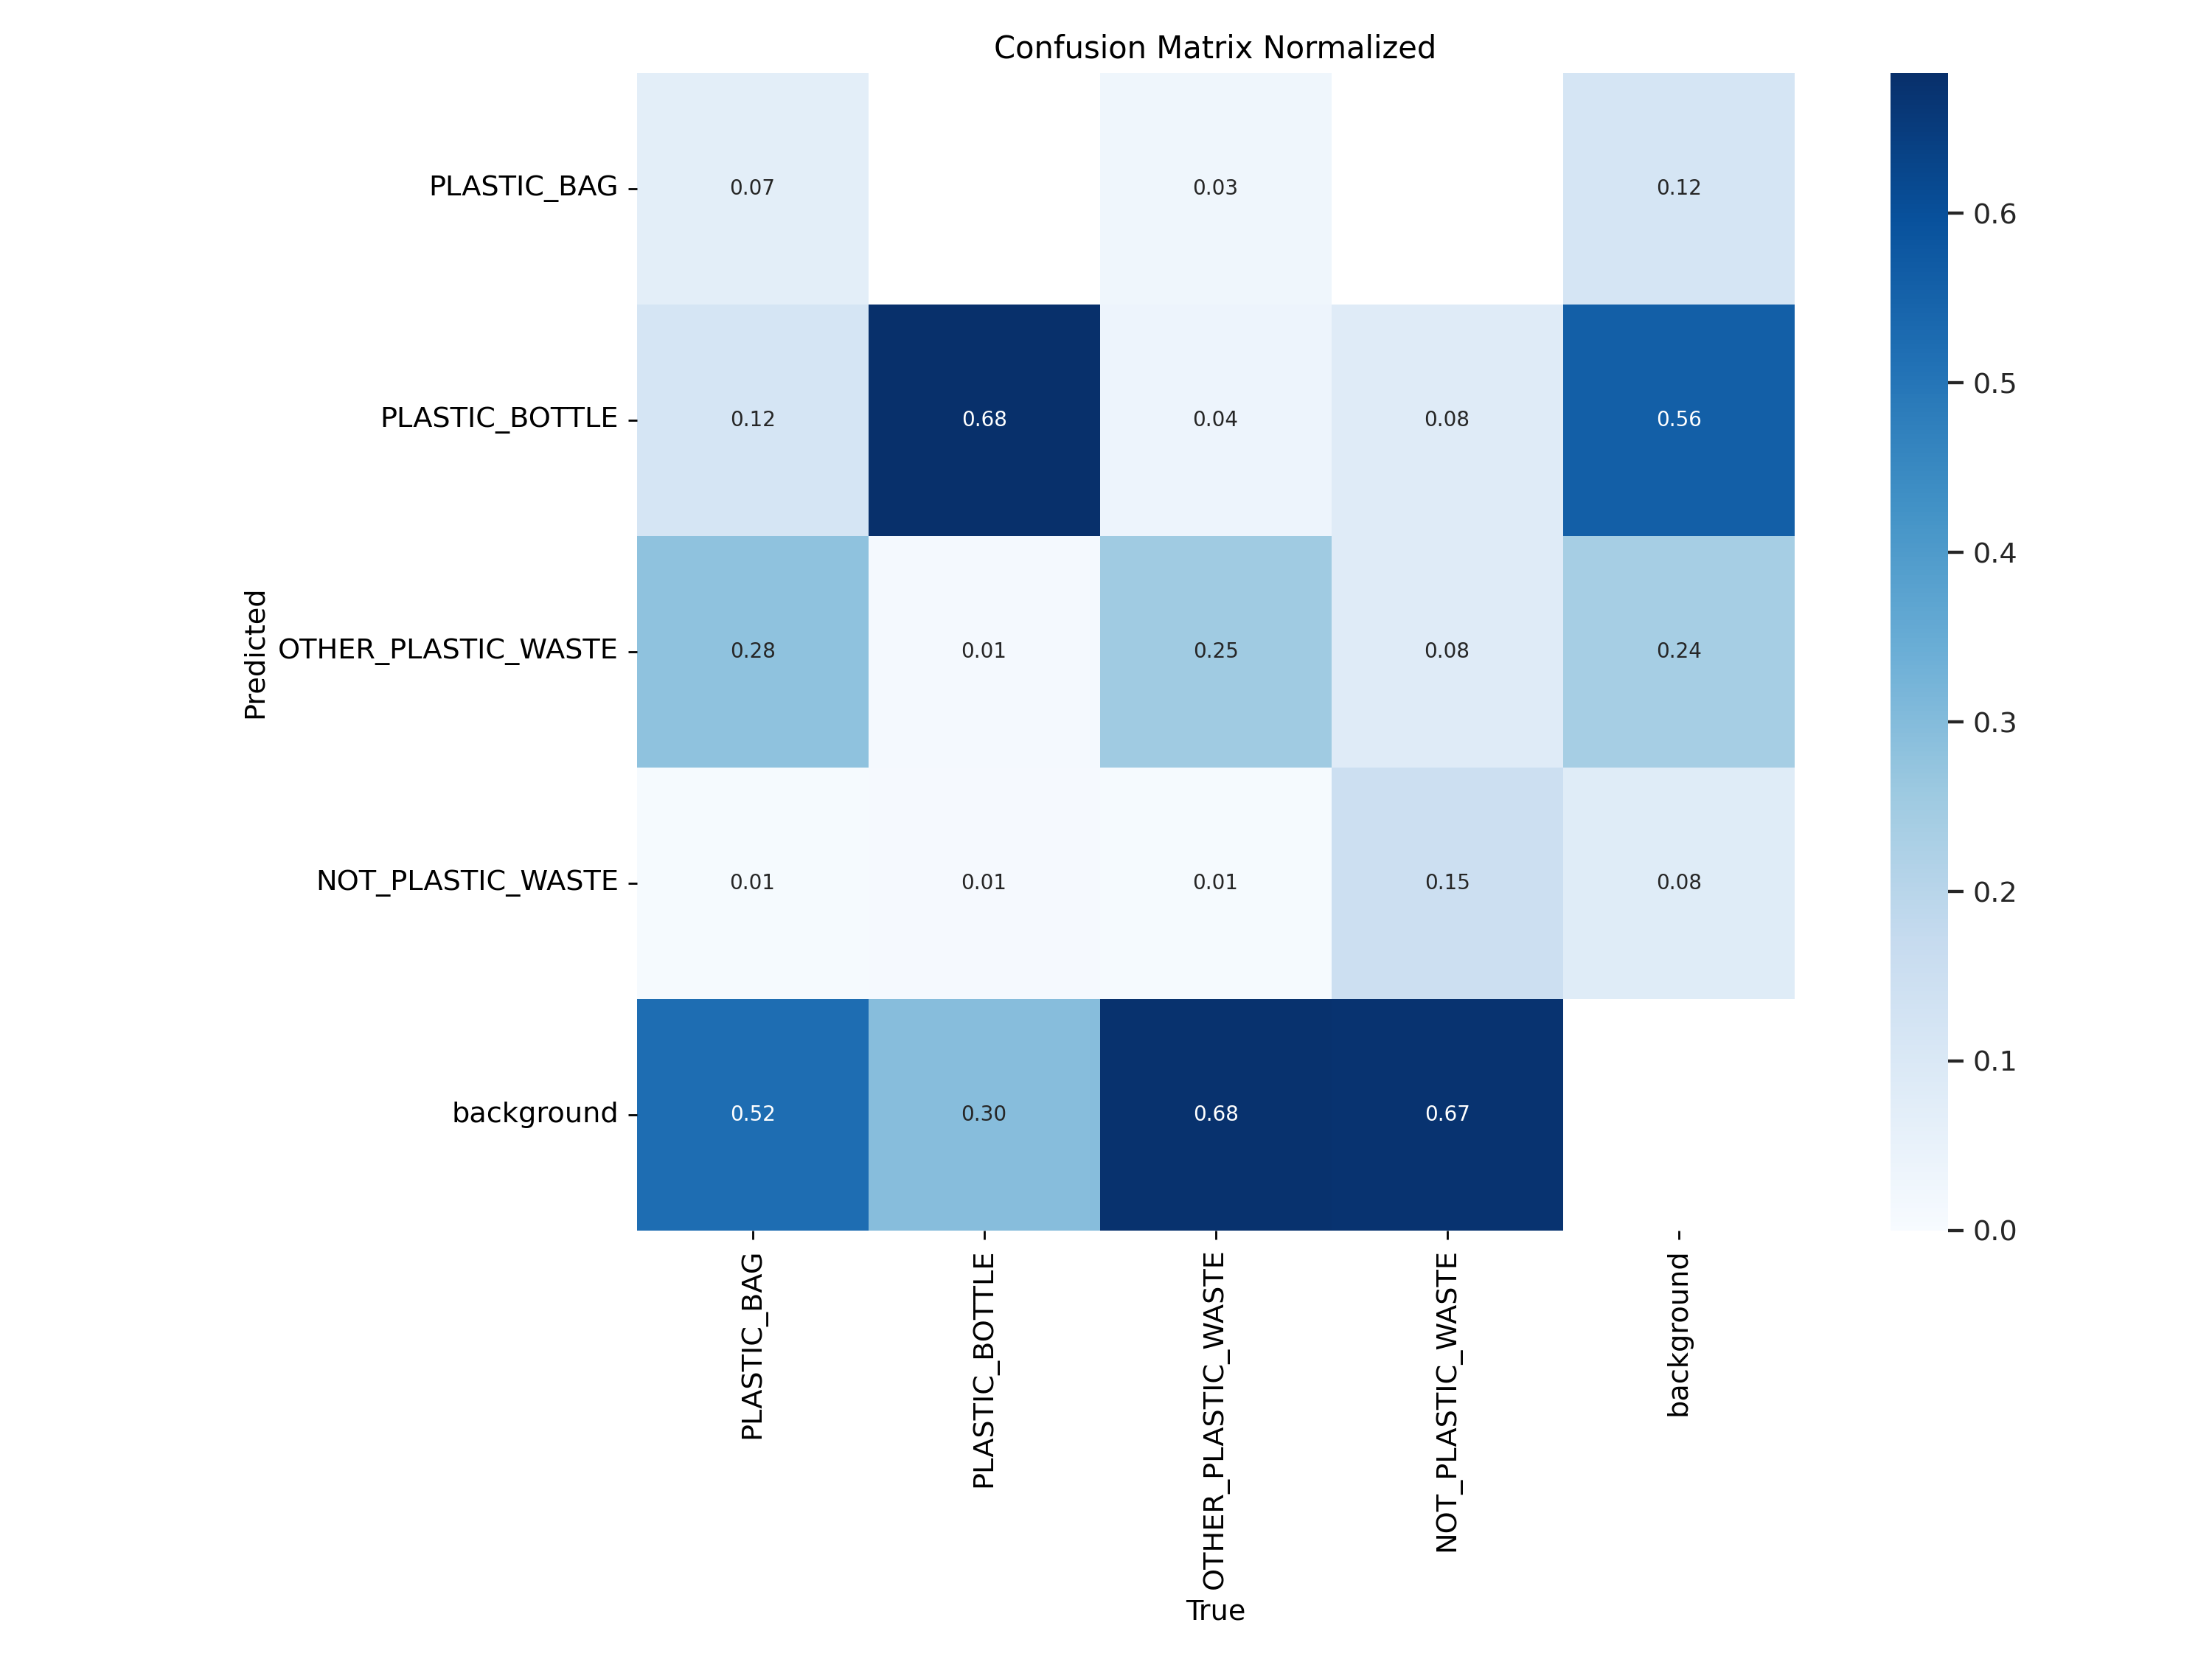
\includegraphics[width=0.9\textwidth]{v_6/small-tune-2.0/confusion_matrix_normalized.png}
        \subcaption{Small}
        \label{fig:v6-7.2}
    \end{subfigure}
    \begin{subfigure}{.49\textwidth}
        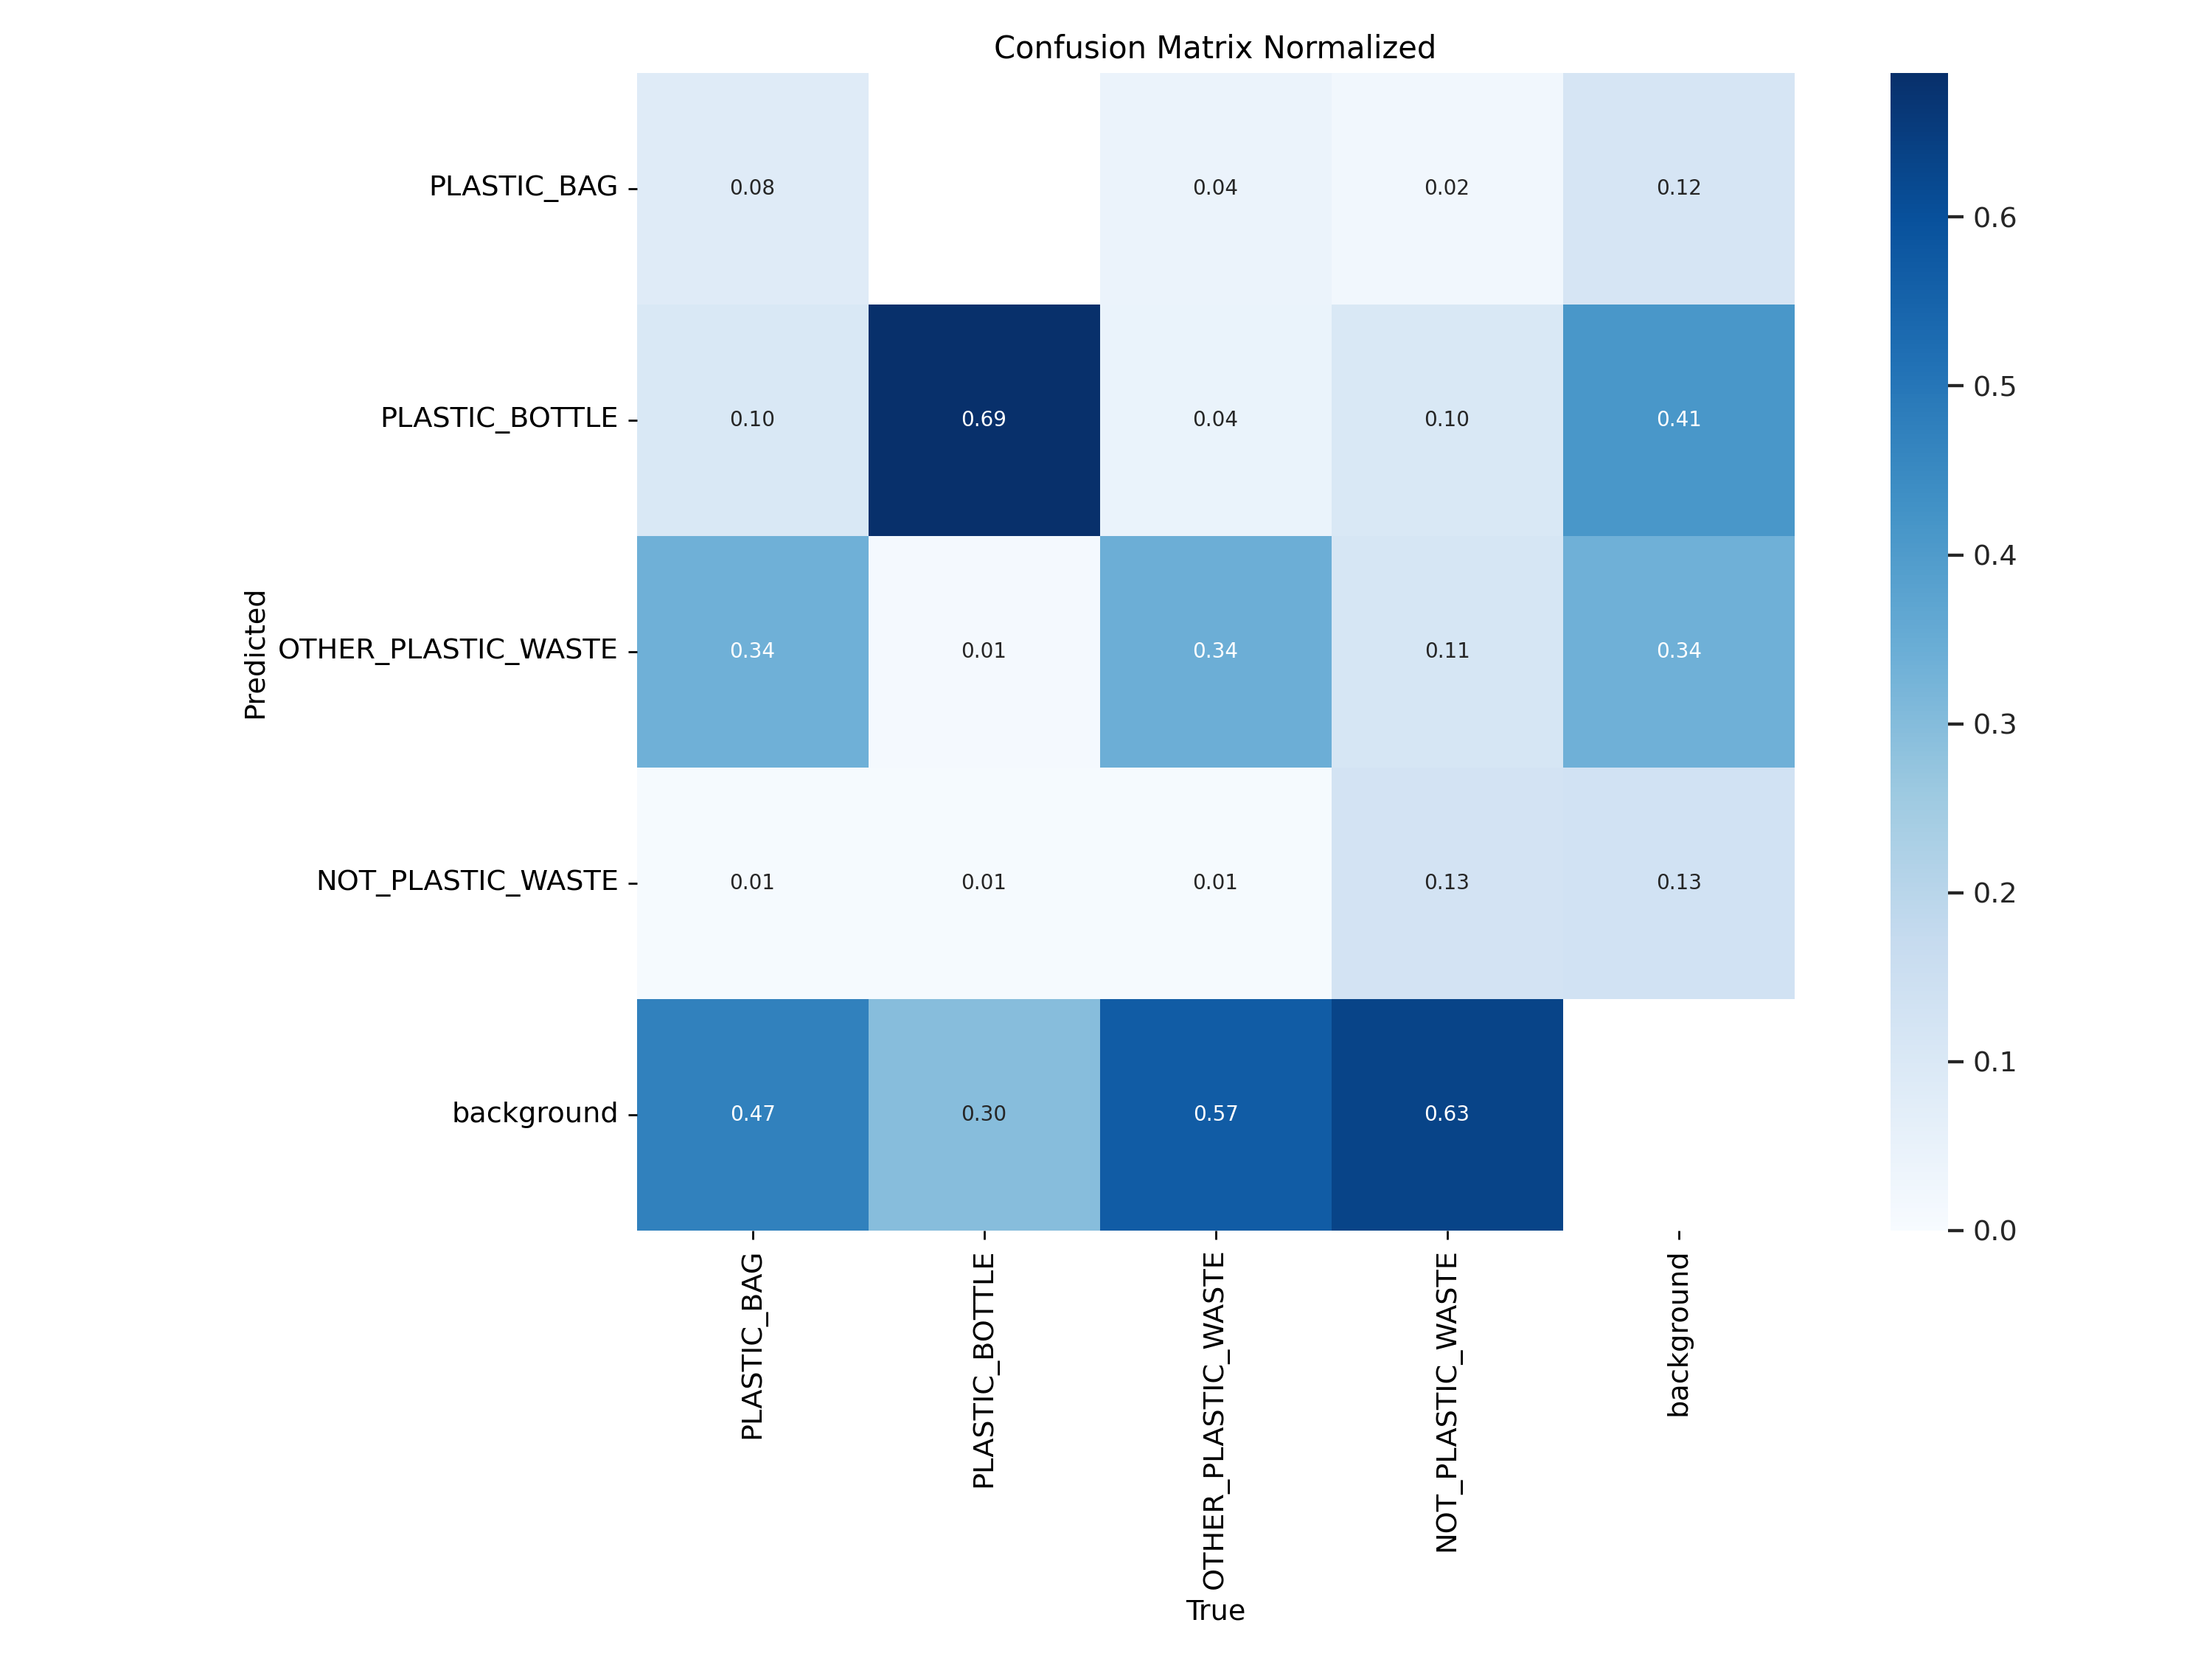
\includegraphics[width=0.9\textwidth]{v_6/medium-tune-2.0/confusion_matrix_normalized.png}
        \subcaption{Medium}
        \label{fig:v6-7.3}
    \end{subfigure}
    \caption{Comparazione tra le matrici di confusione normalizzate
    dei modelli \textit{size}\texttt{-tune-2.0}}
    \label{fig:v6-7}
\end{figure}

\section{Commento risultati e conclusioni}

Ultima sezione da scrivere

% \tableofcontents
% \listoffigures
% \listoftables
\end{document}